\documentclass[t]{beamer}

\usepackage[T1]{fontenc}
\usepackage[utf8]{inputenc}
\usepackage{upquote}


\usepackage{array}
\usepackage{ragged2e}

\usepackage[ngerman,english]{babel}
\usepackage[babel,german=quotes]{csquotes}
\usepackage{graphicx}
\usepackage{textpos}
\usepackage{tikz}
\usepackage{subfig}

\usetikzlibrary{shapes.arrows,calc,decorations.pathmorphing}
\usetikzlibrary{arrows.meta,shapes.misc}
\usetikzlibrary{fit}

%%\usepackage{gitinfo}
\usepackage{shadowtext}

\usetheme{-tud-4-3}
\newcommand{\titel}{Introduction to Meshes}
\newcommand{\titelkurz}{Introduction to Meshes}
\newcommand{\vortragender}{Raphael M\"unster}
\newcommand{\koautoren}{}
\newcommand{\ortdatum}{\today}

% Title page
\title[\titelkurz]{\titel}
\author{Raphael M\"unster}
\date{\ortdatum\\[-0.2cm]}
\institute{TU Dortmund - Lecture Sim Tech}

% ------------------------------------------------------------------------------------
% VORTRAG ESCO 2012     FRIEDRICH-ALEXANDER-UNIVERSITAET ERLANGEN-NUERNBERG
% ------------------------------------------------------------------------------------
%     erstellt von Christopher Basting, 21. Juni 2012
% ------------------------------------------------------------------------------------
% abbrev.tex
% ------------------------------------------------------------------------------------

% Mathe spezifische Packages
\usepackage{amsmath,amsfonts}
\usepackage{dsfont}

\renewcommand{\d}{{\rm d}} % d fuer dx bei Ableitungen / Integralen
\newcommand{\gdw}{\Leftrightarrow} % <=>
\newcommand{\x}{\cdot}
\newcommand{\ma}{\left( \begin{array}{*{19}{c}}} % Matrix oeffnen
\newcommand{\me}{\end{array}\right)} % Matrix schliessen
\newcommand{\mA}{\left[ \begin{array}{*{19}{c}}} % Matrix oeffnen
\newcommand{\mE}{\end{array}\right]} % Matrix schliessen
\newcommand{\C}{\mathds{C}}
\newcommand{\E}{\mathds{1}}
\newcommand{\F}{\mathds{F}}
\newcommand{\K}{\mathds{K}}
\newcommand{\N}{\mathds{N}}
\newcommand{\Q}{\mathds{Q}}
\newcommand{\R}{\mathds{R}}
\newcommand{\Z}{\mathds{Z}}
\newcommand{\id}{\mathds{1}}
\renewcommand{\d}{\,{\rm d}}
\newcommand{\D}{{\rm D}}
\newcommand{\richtig}{\checkmark}
\newcommand{\falsch}{\lightning}
\newcommand{\ra}{\rightarrow}
\newcommand{\Ra}{\Rightarrow}
\newcommand{\la}{\leftarrow}
\newcommand{\La}{\Leftarrow}

\newcommand{\abbildung}[3]{#1 \, : \, #2 \rightarrow #3}
\newcommand{\grad}{\nabla}

%\renewcommand{\phi}{\varphi}
\newcommand{\cL}{\mathcal{L}}
\newcommand{\cO}{\mathcal{O}}

\newcommand{\eps}{\varepsilon}

\renewcommand{\vec}{\bold}
\newcommand{\dist}{{\rm dist}}

\newcommand{\mat}[1]{\textsf{\textbf{#1}}}

\usepackage{amscd,amssymb} 

\providecommand{\abs}[1]{\lvert#1\rvert}
\providecommand{\norm}[1]{\left\lVert#1\right\rVert}
\providecommand{\normNoAdjust}[1]{\lVert#1\rVert}
\providecommand{\transpose}[1]{{#1}^\top}
\providecommand{\inversetranspose}[1]{{#1}^{-\top}}



\shadowoffsetx{0.7pt}
\shadowoffsety{0.7pt}


\newcommand{\itemra}{\item[$\rightarrow$]}
%\newcommand{\TUgreen}{\color{TUgreen}}
\newcommand{\TUgreen}{\color{red}}
\usepackage{hyperref}

\usepackage{listings}
\usepackage{xcolor}

%New colors defined below
\definecolor{codegreen}{rgb}{0,0.6,0}
\definecolor{codegray}{rgb}{0.5,0.5,0.5}
\definecolor{codepurple}{rgb}{0.58,0,0.82}
\definecolor{backcolour}{rgb}{0.95,0.95,0.92}

%Code listing style named "mystyle"
\lstdefinestyle{mystyle}{
  backgroundcolor=\color{TUlightgreen},   commentstyle=\color{codegreen},
  keywordstyle=\color{magenta},
  numberstyle=\tiny\color{codegray},
  stringstyle=\color{codepurple},
  basicstyle=\ttfamily\footnotesize,
  breakatwhitespace=false,         
  breaklines=true,                 
  captionpos=b,                    
  keepspaces=true,                 
  numbers=none,                    
  numbersep=5pt,                  
  showspaces=false,                
  showstringspaces=false,
  showtabs=false,                  
  tabsize=2
}

%"mystyle" code listing set
\lstset{style=mystyle}



\lstset{breaklines=true,      % sets automatic line breaking
basicstyle=\ttfamily\LARGE,
language=TeX,
escapechar=@
}

\usepackage{fancybox, graphicx}

\usepackage{lmodern}

% Einige Befehle (s. Thomas Rohkaemper's Slides)
\definecolor{darkgray}{gray}{0.3}
\newcommand{\kommandozeile}[1]{{{\ttfamily\bfseries \color{white}\colorbox{black}{#1}}}}
\newcommand{\dateiname}[1]{{\ttfamily\bfseries \color{red}#1}}
\newcommand{\emphword}[1]{{\color{red}#1}}
\newcommand{\keyword}[1]{\texttt{\color{blue}#1}}
\newcommand{\emphkeyword}[1]{\texttt{\color{red}#1}}
\newcommand{\befehl}[1]{\texttt{\color{blue}\symbol{`\\}#1}}
\newcommand{\tabitem}{~~\llap{\color{red}\textbullet}~~}

\newcommand{\latexBeispielDatei}[2]{
	\begin{columns}[T]
		\begin{column}{0.54\textwidth}
			\begin{block}{#1}
				\lstinputlisting{#2.tex}
			\end{block}
		\end{column}
		\begin{column}{0.44\textwidth} \vspace{-2.5cm}
			\shadowbox{\includegraphics[width=0.9\textwidth]{#2.pdf}}
		\end{column}
	\end{columns}
}

\newcommand{\latexBeispielDateiCodeAnmerkungen}[3]{
	\begin{columns}[T]
		\begin{column}{0.54\textwidth}
			\begin{block}{#1}
				\lstinputlisting{#2.tex}
			\end{block}
		\end{column}
		\begin{column}{0.44\textwidth}
			#3
		\end{column}
	\end{columns}
}

\newcommand{\latexBeispielDateiKlein}[2]{
	\begin{columns}[T]
		\begin{column}{0.54\textwidth}
			\begin{block}{#1}
				\lstinputlisting[basicstyle=\ttfamily\large]{#2.tex}
			\end{block}
		\end{column}
		\begin{column}{0.44\textwidth} \vspace{-2.5cm}
			\shadowbox{\includegraphics[width=0.9\textwidth]{#2.pdf}}
		\end{column}
	\end{columns}
}


\newcommand{\latexBeispielDirekt}[2]{
	\begin{columns}[c]
		\begin{column}{0.54\textwidth}
			\begin{block}{#1}
			\lstinputlisting{#2}
			\end{block}
		\end{column}
		\begin{column}{0.44\textwidth}
			\shadowbox{\begin{minipage}{0.99\textwidth} \input{#2} \end{minipage}}
		\end{column}
	\end{columns}
}

\newcommand{\latexBeispielDirektKlein}[2]{
	\begin{columns}[c]
		\begin{column}{0.54\textwidth}
			\begin{block}{#1}
			\lstinputlisting[basicstyle=\ttfamily\large]{#2}
			\end{block}
		\end{column}
		\begin{column}{0.44\textwidth}
			\shadowbox{\begin{minipage}{0.99\textwidth} \input{#2} \end{minipage}}
		\end{column}
	\end{columns}
}

\newcommand{\latexBeispielDirektFake}[3]{
	\begin{columns}[c]
		\begin{column}{0.54\textwidth}
			\begin{block}{#1}
			\lstinputlisting{#2}
			\end{block}
		\end{column}
		\begin{column}{0.44\textwidth}
			\shadowbox{\begin{minipage}{0.99\textwidth} #3 \end{minipage}}
		\end{column}
	\end{columns}
}

\begin{document}

%
%
%%%%%%%%%%%%%%%%%%%%%%%%%%%%%%%%%%%%%%%%%%%%%%%%%%%%%%%%%%%%%%%%%%%%%%%%%%%%%
%
%
% Kopf- und Fußzeile abschalten
\frame[plain,c]{\titlepage}

% ab jetzt Autoren ohne Unterstreichung des Vortragenden
\author{\vortragender}

% keine eigene Seite für jede Section einblenden (kann mit \activateOwnSectionPage rückgängig gemacht werden)
\deactivateOwnSectionPage 


%%%%%%%%%%%%%%%%%%%%%%%%%%%%%%%%%%%%%%%%%%%%%%%%%%%%%%%%%%%%%%%%%%%%%%%%%%%%%
% N O R M A L E   U N I - V E R S I O N
%%%%%%%%%%%%%%%%%%%%%%%%%%%%%%%%%%%%%%%%%%%%%%%%%%%%%%%%%%%%%%%%%%%%%%%%%%%%%
\section{Introduction}
\begin{frame}
	\frametitle{Basic 'Mesh' Terminology}
  \begin{itemize}
		\item \keyword{Mesh Generation} (\keyword{Meshing}) is the act of creating a mesh for a computing task
		\item Generally a \keyword{Mesh} is a discretized representation of a geometry 
		\item Meshes are used in FEM, FV, FD, Physics Simulators (Rigid or Soft Bodies), CAD, Rendering, 3D Printing,...
		\item Mesh Generation software is often specialized for a certain target application ($\uparrow$)
		\item Larger software packages often have mesh generation software included as a component of the package
		\item Meshes used for computational tasks need to fulfill certain \keyword{quality criteria}
		\item \keyword{Quality criteria} are checked before use to prevent unnecessary failure and remeshing
		\item \keyword{Mesh Data Structures}, \keyword{Mesh Formats} and \keyword{Mesh Conversion} are essential components of the meshing workflow
  \end{itemize}	
\end{frame}

\begin{frame}
	\frametitle{Mesh Generation}
  \begin{itemize}
		\item Mesh Generation is a huge/important aspect of simulation (for mesh-based methods of course)
		\item Manual, automatic and hybrid (combination of manual + automatic) mesh generation methods
		\item Computational domains have different components that can be meshed differently
		\item Meshing of inflow, outflow, wall, embedded geometry or other special function components of the domain
		\item Surface meshes (usually surface triangulations) are frequently used to simulate flow around objects
		\item Create a mesh that fulfills the quality criteria for the designated computation task
		\item Involves scientific disciplines such as computational geometry, differential geometry, geometric modeling, optimization, etc.
  \end{itemize}	
\end{frame}

\begin{frame}
	\frametitle{Mesh Nomenclature}
  \begin{itemize}
		\item Focus on 2D Meshes, 3D Surface/Volume meshes
		\item Basic topological terminology and theory of meshes in the works of Kinsey \cite{kinsey1993topology} and 
Edelsbrunner\cite{Edelsbrunner:2006:GTM:1137760}.		
  \end{itemize}		
  \begin{block}{Definition: Mesh or Cell Complex}
  A mesh $\mathcal M$ is composed of a finite number of $n$-dimensional cells: 
	\begin{align*}
   \mathcal M =\{\omega : \omega \text{ is a element}\}.  
  \end{align*}
  \end{block}	
  \begin{itemize}
		\item \keyword{Cell Complex} is a common alternative term for mesh in literature
		\item Term is used computational geometry package \keyword{CGAL} and implemented as a data structure
  \end{itemize}			
\end{frame}

\begin{frame}
  \frametitle{Cell Complex Example}
	\begin{block}{Hexahedron Example}
   The hexahedron is composed of one 3-dimensional element/cell, the 3-dimensional cell is composed of six 2-dimensional cells, the facets. The facets are
	 composed of the 1-cells called edges/segments describing their boundaries. The endpoints of the edges are the eight 0-dimensional cells, the vertices.
	\end{block}
    \begin{center}
      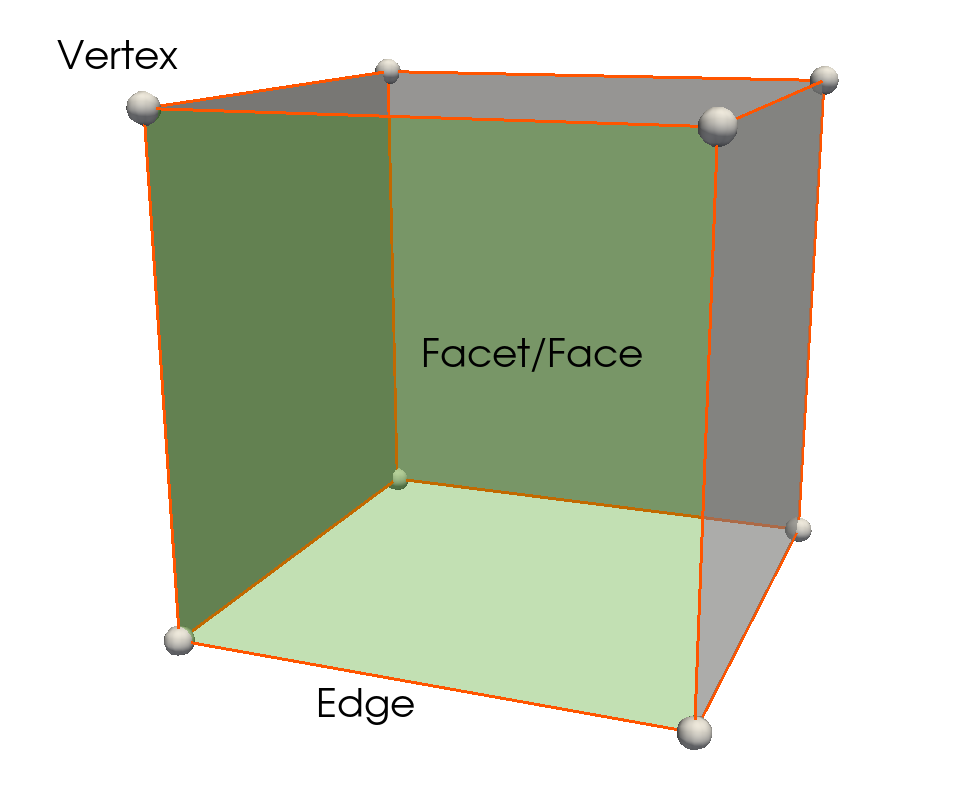
\includegraphics[width=0.4\textwidth]{screenshots/hexa-cell2.png}
    \end{center}			
\end{frame}

\begin{frame}
  \frametitle{Dimension of a Cell Complex}
 	\begin{block}{Dimension of a Cell Complex}
	The dimension of a mesh is equal to the highest cell dimension in the mesh.
   A cell of a mesh is the mesh component the inner of which is homeomorphic to the inner set of an $n$-dimensional disk.  
	\end{block}
  \begin{itemize}
		\item The boundary of a cell is composed of cells of lower dimension, these lower dimensional cell boundaries are
 called \keyword{faces} or \keyword{facets}.
		\item For these relationship between faces and cells we can also use the notation $\sigma < \tau$ to indicate that $\sigma$ is a face of cell $\tau$.
		\item A polyhedron for example is a cell that is composed of polygonal faces(two-dimensional cells), edges (one-dimensional cells) and vertices (zero-dimensional cells).
  \end{itemize}	
\end{frame}

\begin{frame}
  \frametitle{Structure of a Cell Complex}
In order to construct a mesh we combine and connect cells of equal dimension: vertices are connected to vertices and edges are connected to \keyword{adjacent} edges. 
 	\begin{block}{Dimension of a Cell Complex}
By $|\mathcal M|$ we refer to the set of points of mesh $\mathcal M$:	
\begin{align*}
  |\mathcal M|=\{\vec{x} : \vec{x} \in \sigma \in \mathcal M, \text{$\sigma$ is a cell in $\mathcal M$.}\}  
\end{align*}
	\end{block}
  \begin{itemize}
		\item $|\mathcal M|$ is also called the underlying space of $\mathcal M$
		\item For every vertex in $|\mathcal M|$ a defined neighborhood relationship has to exist
		\item Neighborhood in a 2-cell complex:
		\begin{itemize}
			\item Vertex neighborhoods over edge connections
			\item Facet neighborhood over edges			
			\item Facet neighborhood over vertices
			\item ...									
		\end{itemize}				
  \end{itemize}		
\end{frame}

\begin{frame}
  \vspace{-1cm}
  \frametitle{Neighborhoods/Connectivity in a Cell Complex}
		\begin{itemize}
			\item For vertex $\vec{v}$ inside of a polygon, the neighborhood of $\vec{v}$ is an arbitrary disk that is entirely located in the inside 
of the polygon. 
			\item If the vertex $\vec{v}$ is on an edge $\vec{e}$ that was contructed by unification of edges $\vec{e}_0,\dots,\vec{e}_n$ then the corresponding vertex $\vec{v}$ has to be present on every edge $\vec{e}_i$.
			\item Facet neighborhood over vertices
			\item The unification of half-disk neighborhoods of the vertices $\vec{v}_0,\dots,\vec{v}_n$ leads to the neighbor relationship that is
depicted in figure \ref{fig:mesh-neighborhood}.
			\item When $\vec{v}$ is contructed from polygon vertices $\vec{v}_0,\dots,\vec{v}_n$ the neighborhood of $\vec{v}$ is composed of the different disc- or half-disc neighborhoods of $\vec{v}_0,\dots, \vec{v}_n$.  
		\end{itemize}					 
\begin{figure}[h!]
\begin{center}
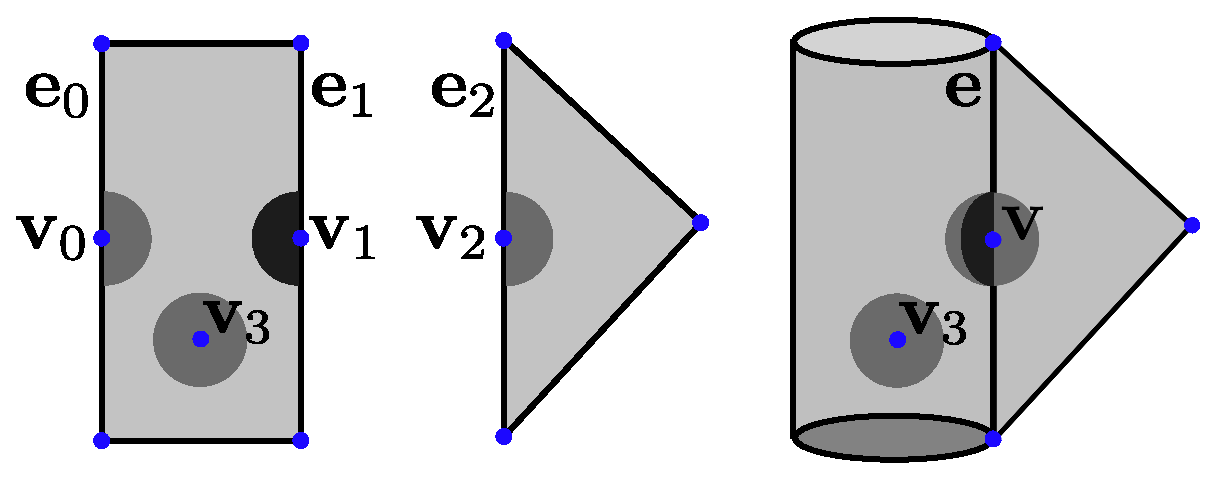
\includegraphics[height=3cm]{screenshots/neighborhood.eps}
\end{center}
\caption{We unify edges $\vec{e}_0$, $\vec{e}_1$ and $\vec{e}_2$, the resulting cell complex or mesh is on the right. The vertex $\vec{v}$ that has been produced by
unifying the other vertices also has a neighborhood that is the result of the unification of $\vec{v}_0$, $\vec{v}_1$ and $\vec{v}_2$ \cite{kinsey1993topology}.}
\label{fig:mesh-neighborhood}
\end{figure}

\end{frame}

\begin{frame}
  \frametitle{Adjacency, Incidence, Valency and Stencil}
From basic graph theory the adjacency and incidency relationships are important for our
considerations:
		\begin{itemize}
			\item \keyword{Adjacency} is the neighborhood relation between same type mesh components whereas \keyword{incidency} is the neighborhood relation between mesh components of
a different type.
			\item Using this terminology we call two polygons adjacent if there is an edge that is incident to both polygons
							 
 
\item The \keyword{stencil} of a vertex is the set of edges and polygons incident to the vertex:
\begin{align*}
  Stencil \text{ } \tau = \{\sigma \in K| \tau < \sigma \}
\end{align*}
\item The \keyword{degree} or \keyword{valency} of a vertex $\vec{v}$ is the number of vertices $\vec{v}_i$ that is adjacent to $\vec{v}$, meaning there exists an edge that connects $\vec{v}$ to $\vec{v}_i$.
\end{itemize}
\end{frame}

\begin{frame}
  \frametitle{Surface Meshes}
\begin{itemize}
\item Usually a triangulation or quadrangulation of a geometric object
\item In CFD simulations used as:
	\begin{itemize}
	  \item Domain boundaries
	  \item Immersed static objects		
	  \item Immersed dynamic objects				
	\end{itemize}
\item Immersion of surface meshes into CFD simulations usually done by \keyword{Fictitious Domain} Methods (FEATFLOW: \keyword{Fictitious Boundary})
\end{itemize}
\begin{figure}[h!]
\centering
\subfloat[Streamline flowfield around a \newline helix geometry]{ 
 \includegraphics[height=3cm]{Images/helix.eps}
 \label{fig:helix}
}%\hspace{0.1cm}
\subfloat[ Twin screw geometry simulation ]{ 
 \includegraphics[height=3cm]{Images/liquidsolid_intro.eps}
 \label{fig:liquidsolid_intro}
}
\caption{CFD Examples with surface meshes}
\label{fig:liquid-solid}
\end{figure}
\end{frame}

\begin{frame}
\frametitle{Surface Meshes Example}

\begin{figure}[h!]
	\begin{center}
	   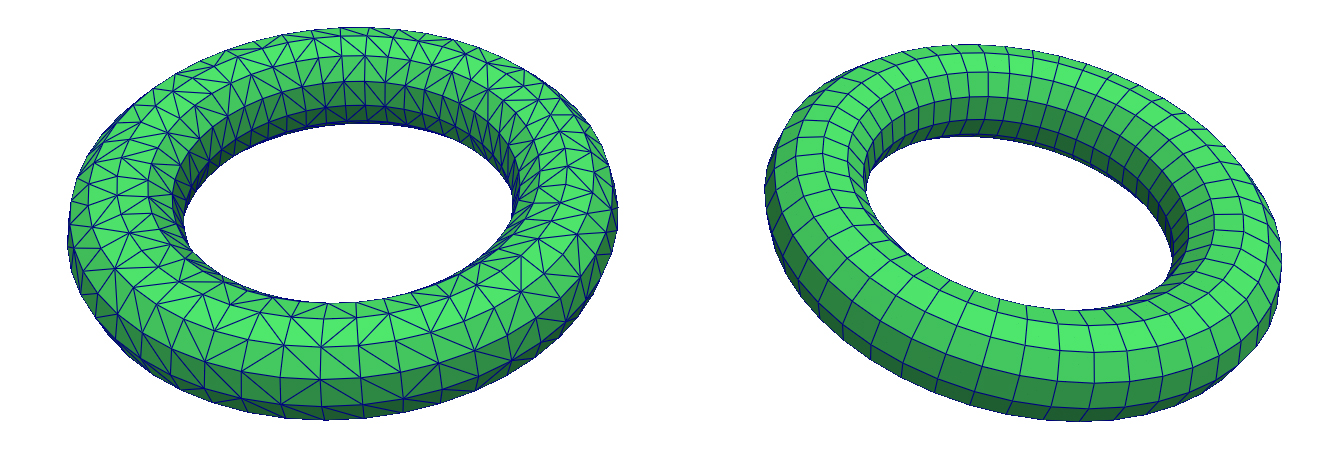
\includegraphics[width=\textwidth]{screenshots/tori.jpg}
	\end{center}
	%\caption{From left to right: manifold surface, non-manifold at an edge and non-manifold at a vertex.}
	\label{fig:tori}
\end{figure}
\end{frame}

\begin{frame}
For multiple tasks surfaces are required to be \keyword{manifolds}:
\begin{itemize}
\item An $n$-dimensional manifold is a topological space in which every vertex has a neighborhood that is topologically equivalent to an open $n$-dimensional disk. 
\item Two distinct points have disjoint neighborhoods, a surface is a \keyword{2-manifold} 
\item If a manifold has a boundary then there exist vertices that have a neighborhood that is topologically equivalent to an open $n$-dimensional disk or half-disk
\item If a vertex has neither an open disk nor open half-disk neighborhood then it is called \keyword{non-manifold}
\item If a surface has one or more non-manifold vertices then the surface is called a non-manifold surface
\end{itemize}
\begin{figure}[h!]
\begin{center}
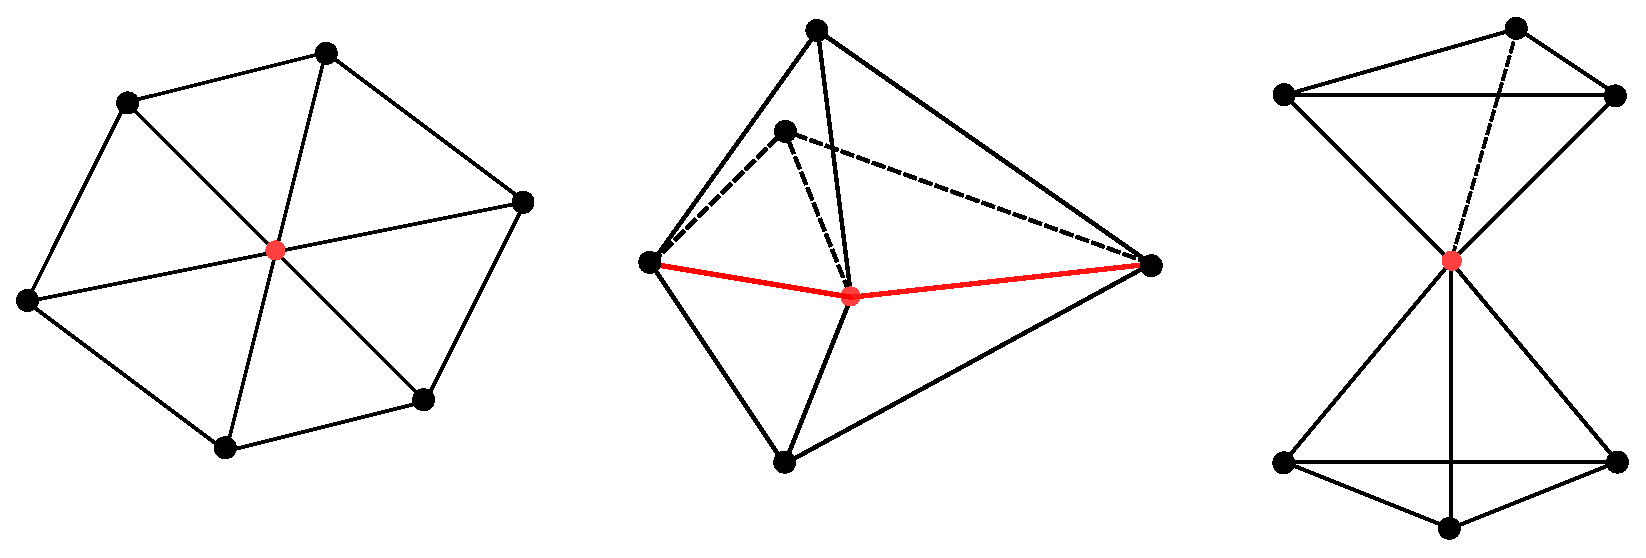
\includegraphics[height=3cm]{screenshots/non_manifolds.eps}
\end{center}
\caption{From left to right: manifold surface, non-manifold at an edge and non-manifold at a vertex.}
\label{fig:non-manifold}
\end{figure}
\end{frame}

\begin{frame}
A bounded manifold can be either \keyword{orientable} or \keyword{non-orientable}
\begin{itemize}
\item A surface is orientable if it does not contain a \keyword{Moebius Strip} \cite{Edelsbrunner:2006:GTM:1137760}.
\item A Moebius Strip can be explained by considering an $(n+1)$-dimensional object moving continiously along an n-manifold
\item If the the object is located on one side of the n-manifold and on its travelling path it revisits a neighborhood, but this time from the other side, then this path is a Moebius Strip and the surface is not orientable
\item The surfaces used to construct two-dimensional meshes are orientable, the cells of these meshes are triangles or quadrilaterals, which are connected by vertices or edges
\item Thus, there should be no isolated vertices or edges that are not part of a polygon in our mesh according to this terminology
\end{itemize}

\begin{figure}[h!]
 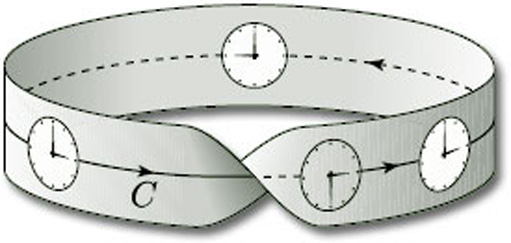
\includegraphics[height=3cm]{screenshots/moebius.jpg}
 \label{fig:moebius-render}
\caption{A Moebius Strip can be created by twisting and connecting the edges of a planar strip, see also \cite{Edelsbrunner:2006:GTM:1137760,kinsey1993topology}.}
\label{fig:moebius}
\end{figure}
\end{frame}

\begin{frame}
\frametitle{Software For Generation and Processing of Surface Meshes}

\begin{itemize}
	\item \keyword{Blender}: Creation, manipulation, format conversion, visualization, analysis, postprocessing, open-source, Python scripting
	\item \keyword{Autodesk 3DS Max}: As Blender, but commercial, a bit more advanced manipulation features, proprietary scripting language, Windows only
	\item \keyword{Meshlab}: Mesh analysis, correction of mesh defects, calculation of various mesh properties and indicators
	\item \keyword{Autodesk Inventor}: CAD, creation of meshes from \keyword{NURBS}-Surfaces \cite{NURBSBOOK}
	\item \keyword{FreeCAD}: Open-source CAD program, less functions than Inventor
	\item \keyword{CGAL}: Open-source modern C++ software library for creation, manipulation, analysis, geometric algorithms,...
	\item \keyword{OpenMesh}: Open-source modern C++ data structure for surface meshes from RWTHA 	
\end{itemize}

\end{frame}

\begin{frame}{Data Formats for Surface Meshes}
    \begin{columns}
        \column{0.5\textwidth}{
            \begin{exampleblock}{Element-List}
                \begin{itemize}
                  \item STL
                \end{itemize}
								Properties
                \begin{itemize}
                  \item Stores each element and vertex coordinates
                  \item Redundant repetition of coordinates									
                  \item Problem: Vertex coordinates may not coincide $\rightarrow$ invalid mesh										
                  \item Can store additional properties									
                  \item Main usage for graphics renderings									
                \end{itemize}								
            \end{exampleblock}       }
        \column{0.5\textwidth}{
            \begin{alertblock}{Connectivity-Based}
                \begin{itemize}
                  \item Wavefront OBJ		
                  \item OFF
                  \item Stanford PLY
                  \item VTK									
                \end{itemize}
								Properties:
                \begin{itemize}
                  \item List of vertices, followed by list of elements with vertex indices
									\item more storage efficient
                  \item Some formats allow to store additional properties
                \end{itemize}								
            \end{alertblock}       }
    \end{columns}
\end{frame}

\begin{frame}
\frametitle{OpenMesh - A Surface Mesh Data Structure}
\begin{itemize}
\item \url{https://www.graphics.rwth-aachen.de/software/openmesh/}
\item Uses the efficient halfedge (or winged edge) to the mesh and the connectivity
\item Iterators allow the user to iterate through vertices, edges, faces
\item Circulators allow the user to:
\begin{itemize}
\item iterate over all neighboring vertices of a vertex
\item iterate over all incident edges of a vertex
\item iterate over all faces attached to a vertex
\item iterate over a face's vertices
\item iterate over the face's incident edges
\item iterate over the adjacent faces
\end{itemize}
\item Store user-defined traits in vertices, edges, halfedges, faces	
\item STL-like usage
\end{itemize}								
\end{frame}

\begin{frame}
\frametitle{OpenMesh - The Halfedge Data Structure}
\begin{figure}[h!]
 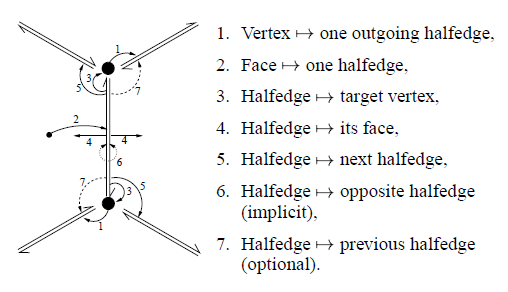
\includegraphics[width=0.8\textwidth]{screenshots/half-edge.png}
\caption{The OpenMesh Half-Edge Data Structure \cite{kobbelt2002openmesh}.}
\end{figure}
\end{frame}

\begin{frame}[fragile]

    \begin{lstlisting}[language=C++]
MyMesh mesh;
for(MyMesh::FaceIter f_it = mesh.faces_begin(); f_it != mesh.faces_end(); ++f_it) {
    std::cout << "The face's valence is " 
		          << mesh.valence( *f_it ) 
							<< std::endl;
}\end{lstlisting}     

\begin{lstlisting}[language=C++]
MyMesh mesh;
for (MyMesh::VertexIter v_it=mesh.vertices_sbegin(); v_it!=mesh.vertices_end(); ++v_it) {
  // circulate around the current vertex
  for (MyMesh::VertexVertexIter vv_it=mesh.vv_iter(*v_it); vv_it.is_valid(); ++vv_it)
  {
    // do something with e.g. mesh.point(*vv_it)
  }
}\end{lstlisting}     
\end{frame}

\begin{frame}
%\frametitle{OpenMesh - The Halfedge Data Structure}
\begin{figure}[h!]
 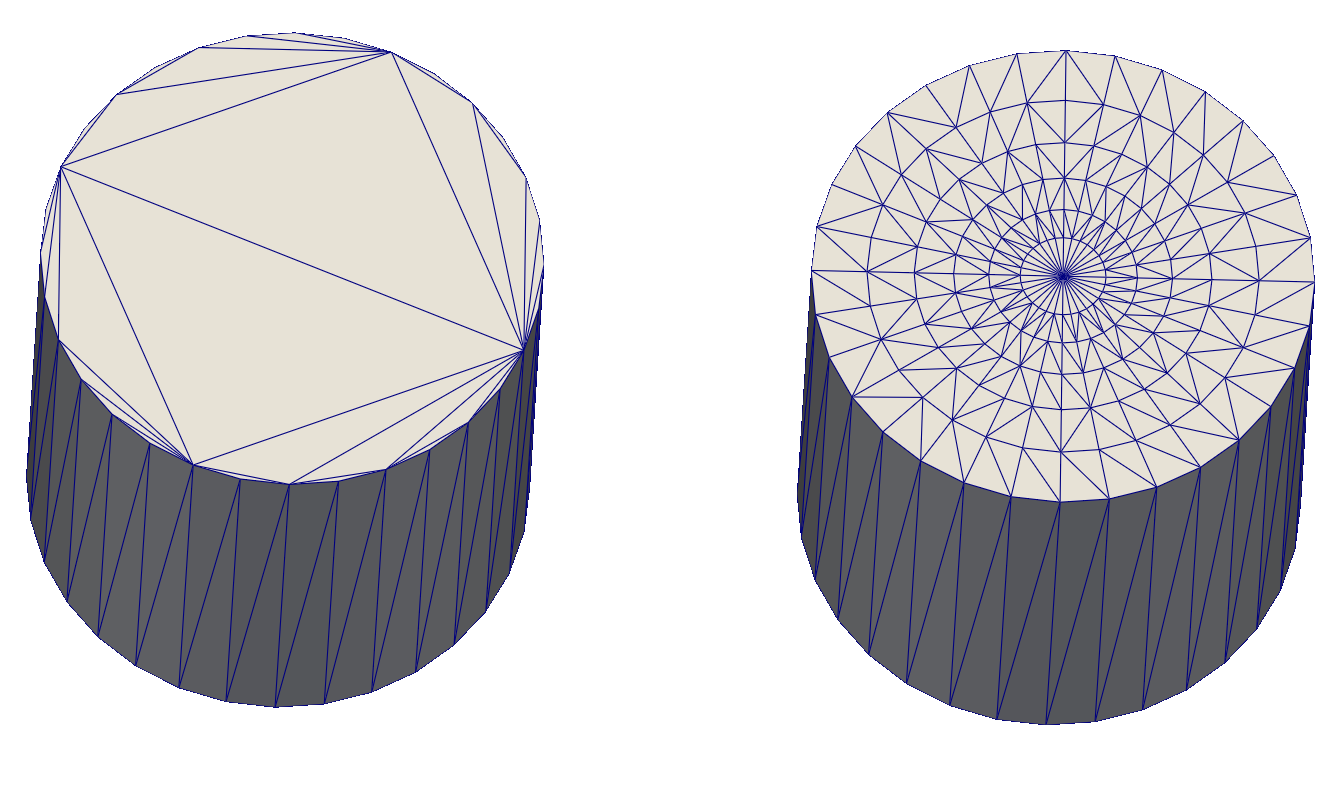
\includegraphics[width=0.8\textwidth]{screenshots/tria-quality.png}
\caption{Triangulations of a Cylinder}
\end{figure}
\end{frame}

\begin{frame}
\frametitle{Meshes for Numerical Simulations}
\begin{itemize}
\item Used to solve discretized PDEs on a computational domain
\item Used i.e. in Finite Volume method (OpenFOAM) and the Finite-Element method
\item Meshes can roughly be grouped into \keyword{structured} and \keyword{unstructured meshes}
\item Meshes need to fulfill quality criteria to facilitate solver convergence
\item Some solvers require special meshes: \keyword{Geometric Multigrid} $\rightarrow$ \keyword{Hierarchical Mesh}
\item Based on the solvers complexity the compute time increases with the degree of mesh refinement (number of elements)
\item \keyword{Domain decomposition} can be used to parallelize the simulation by distributing the subdomains to different processors
\end{itemize}
\end{frame}

\begin{frame}
\frametitle{Structured Meshes}
\begin{itemize}
\item In a structured mesh the valency of every vertices is the same (except for boundary vertices)
\item Consequently, the connectivity is also regular
\item In principle the data structure for a 2D or 3D structured mesh can be a simple 2D or 3D array 
\item Usually not applicable when additional information needs to be stored in the mesh
\item Usual choices of elements in a structured mesh include quadrilateral elements in 2D and hexahedral elements in 3D 
\item Tetrahedrons are possible, but tetrahedrons require more elements to fill a domain with elements
\item Tetrahedrons can represent complex geometries better and automatic mesh generation methods are available
\end{itemize}
\end{frame}

\begin{frame}
There exist different subtypes of structured meshes that are used as computational meshes which mainly include:
\begin{itemize}
\item \keyword{equidistant} cartesian meshes,
\item \keyword{rectilinear} meshes
\item \keyword{curvilinear} meshes 
\end{itemize}
\begin{figure}[h!]
\centering
\subfloat[Equidistant cartesian mesh]{ 
 \includegraphics[height=5cm]{Images/equidistant.pdf}
 \label{fig:equidistant}
}\hspace{0.2cm}
\subfloat[Rectilinear mesh]{ 
 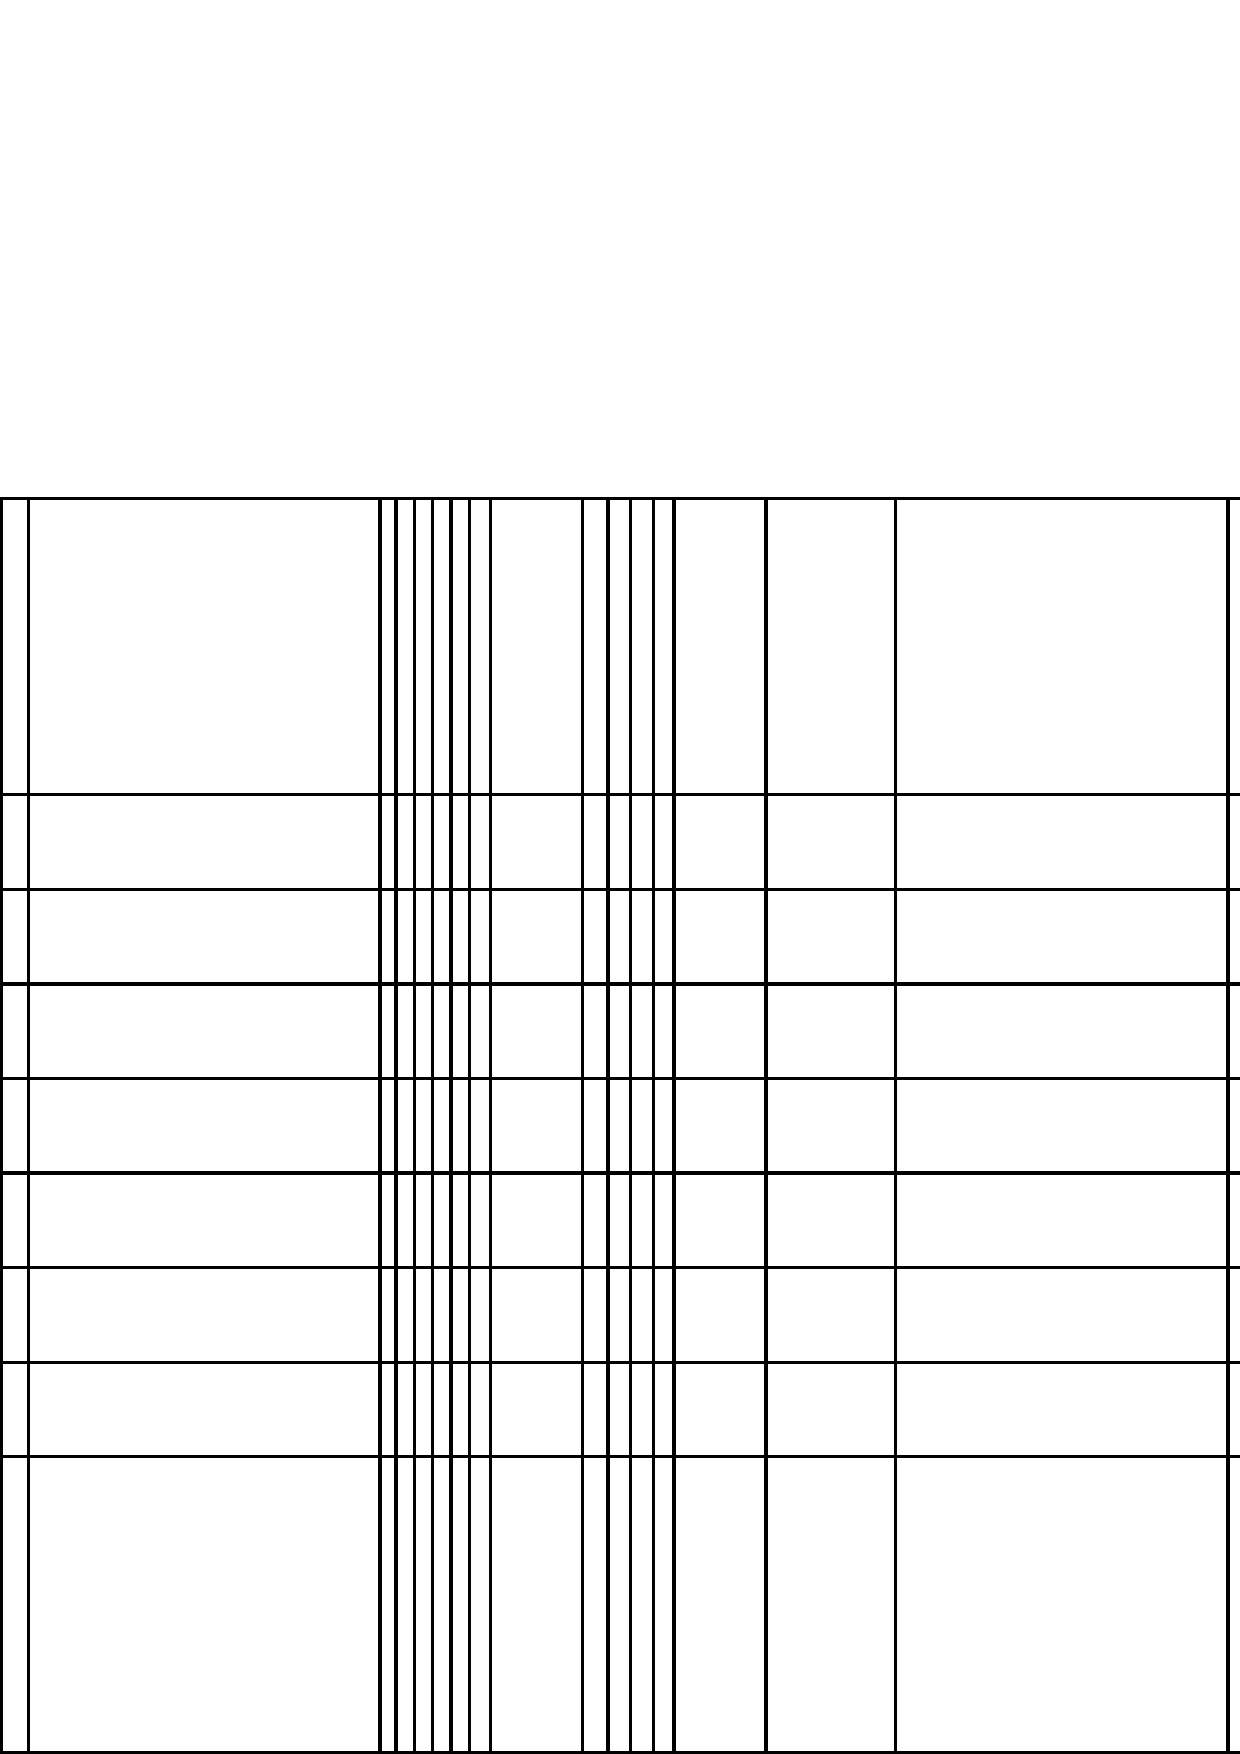
\includegraphics[height=5cm]{Images/rectilinear.pdf}
 \label{fig:rectilinear}
}\hspace{0.2cm}
\subfloat[Curvilinear mesh]{ 
 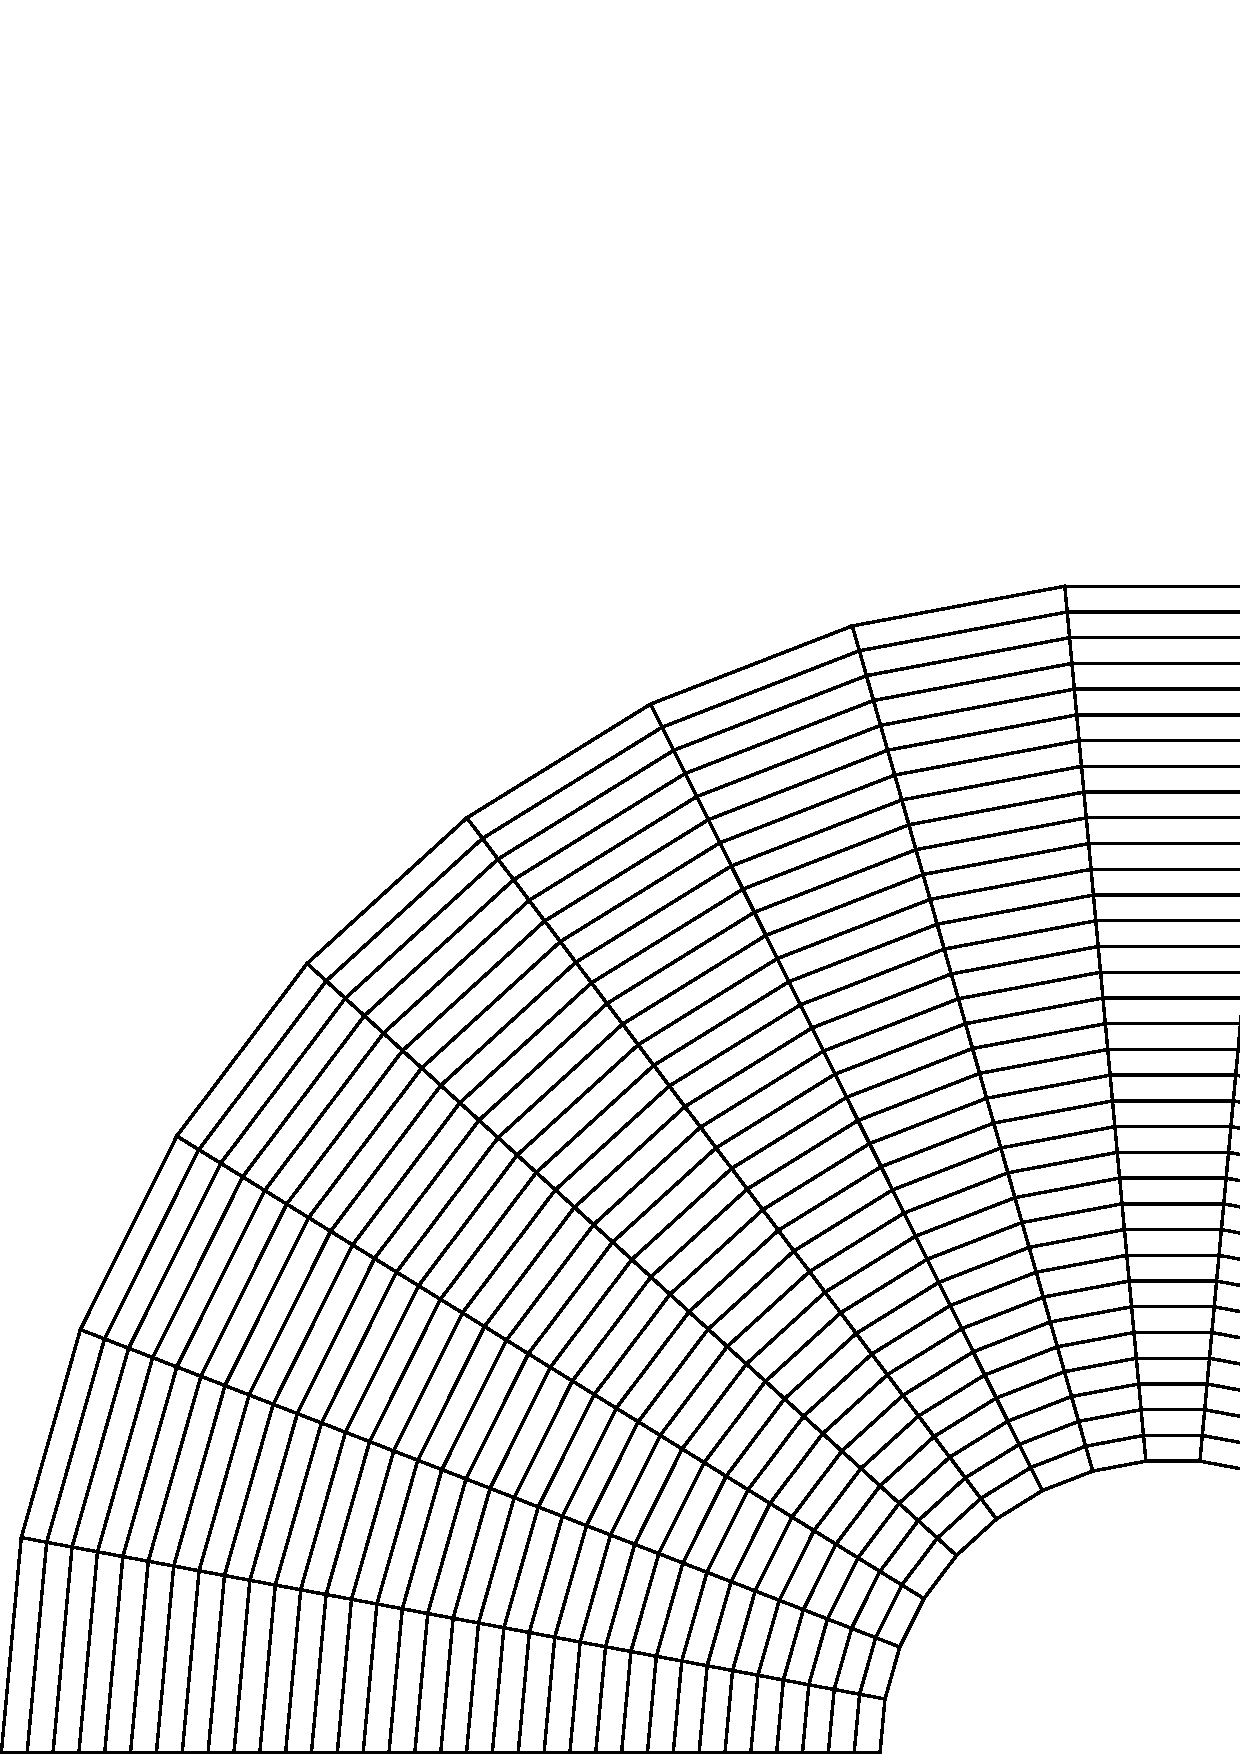
\includegraphics[height=5cm]{Images/curvilinear.pdf}
 \label{fig:curvilinear}
}
\caption{Structured meshes used as computational meshes, from left to right: equidistant structured mesh, rectilinear mesh and curvilinear mesh.}
\label{fig:structured}
\end{figure}
\end{frame}

\begin{frame}
\frametitle{Structured Meshes and Point Location}
The equidistant cartesian meshes have an advantageous property: 
\begin{itemize}
\item They have a uniform element size and it is possible to easily locate an arbitrary point in the mesh
\item Useful for many function evaluation tasks
\item Greatly increases computation speed when using immersed geometries and fictious domain/boundary methods
\end{itemize}
For rectilinear and curvilinear meshes this is also possible, but slightly more difficult. In terms of memory representation of such meshes this means that an element index in a data structure can be efficiently computed based on coordinates in space:
\begin{equation*}
  f: \vec{p} \mapsto i\text{ (array index) }, \vec{p} \in \mathbb{R}^3.
  \label{eq:struct-map}
\end{equation*}
\end{frame}

\begin{frame}
\frametitle{Further Advantages of Structured Meshes}
\begin{itemize}
\item Equidistant cartesian meshes are often used for parallel FV, FEM high performance computing schemes
\item Easy generation, memory access patterns and simple domain decomposition
\item Application of equidistant structured meshes as acceleration structures for geometric computations
\item Employed as a means to subdivide space and thus reduce search domain
\item Spatial subdivision structures intended for acceleration of geometric calculations 
\item Example for geometric queries: visibility determination, point containment, distance or intersection queries
\end{itemize}
\end{frame}

\begin{frame}
\frametitle{Unstructured Meshes}
\begin{itemize}
\item In an unstructured mesh the vertices in general do not have a predefined uniform vertex degree
\item In principle this means that an arbitrary number of cells can be incident to a vertex
\item This is helpful for resolving an immersed geometry because edges, faces can be aligned to the shape of the geometry
\item We call these meshes \keyword{aligned unstructured meshes}
\item Better resolution of flow features and geometry increases the accuracy of the result
\item Unstructured meshes can employ connector elements to gradually increase/reduce the level of refinement in a grid
\end{itemize}
\end{frame}

\begin{frame}
\frametitle{Quality Criteria}
The quality of a mesh depends on the quality of its elements. A variety of mesh quality criteria \cite{kellyansys} exist to measure cell quality:
\begin{itemize}
\item Aspect ratio
\item Angle deviation
\item Corner angle
\item Jacobian ration
\item Inverted cells, self-intersecting cells
\end{itemize}
\end{frame}

\begin{frame}
\begin{figure}[h!]
  \centering
  \subfloat[Example of edge length rations]{ 
    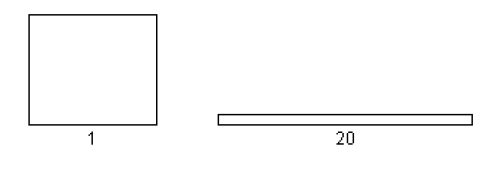
\includegraphics[width=0.75\textwidth]{screenshots/edge-ratio.jpg}
    \label{fig:edgeration}
  }\\
  \subfloat[Examples of angle deviation values]{ 
    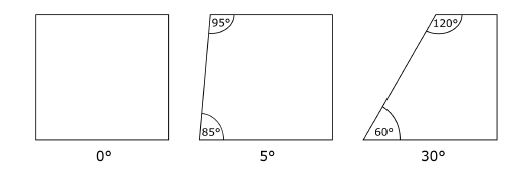
\includegraphics[width=0.75\textwidth]{screenshots/angle-deviation.jpg}
    \label{fig:angledev}
  } 
\end{figure}
\end{frame}

\begin{frame}
\begin{figure}[h!]
  \centering
  \subfloat[Maximum inner angle criterium]{ 
    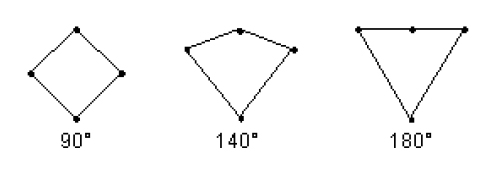
\includegraphics[width=0.75\textwidth]{screenshots/inner-angle.jpg}
    \label{fig:innerangle}
  }\\
  \subfloat[Examples of angle deviation values]{ 
    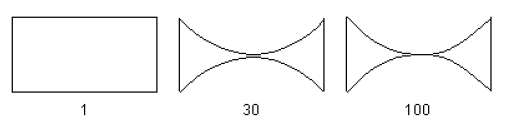
\includegraphics[width=0.75\textwidth]{screenshots/jacobi-deviation.jpg}
    \label{fig:jacobideviation}
  } 
\end{figure}
\end{frame}

\begin{frame}
\begin{figure}[h!]
  \centering  
    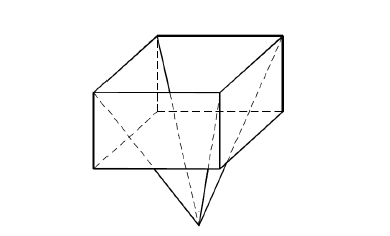
\includegraphics[width=0.75\textwidth]{screenshots/inversion.jpg}
		\caption{Cell self-intersection, inverted cell}
  \label{fig:camaro-mesh}
\end{figure}
\end{frame}

\begin{frame}
\frametitle{Embedding Geometries with the Fictitious Boundary Method}
\begin{itemize}
\item Unstructured meshes in order to better approximate complex-shaped geometries introduces some difficulties as well
\item For Fictitious Boundary type methods one has to know which vertices of the mesh are solid vertices and which are fluid vertices
\item In order to set appropriate boundary conditions an inside/outside indicator function has to be computed
\end{itemize}
\begin{equation*}
 \alpha_{i} (\vec{x}) = 
   \begin{cases}1  &  \mbox{for } \vec{x} \in \Omega_{s}, \\
                0  &  \mbox{for } \vec{x} \in \Omega_{f} \setminus \Omega_s  
   \end{cases}   
\end{equation*}
\begin{itemize}
\item $\Omega_{s}$: solid domain
\item $\Omega_{f}$: fluid domain
\end{itemize}
\end{frame}

%domain areas where a high mesh resolution is required to domain areas where such a high mesh resolution is not needed (see figure \ref{fig:unstructured-fac}). This property is a %clear advantage over structured meshes where the mesh resolution can only be increased globally or by local vertex redistribution without changing the 
%connectivity of the mesh. The . Complex 
%geometries are often explicitly defined by a set of coordinates in space or by an explicit or implicit analytic function. Using an unstructured mesh there is 
%in general no easy way to introduce a mapping from positions in space to element indices in computer memory. Which means that calculations that involve geometric 
%information about the object that is represented by the mesh may need to resort to exhaustive search procedures if no measure are taken to add this feature to the 
%class of unstructured meshes. Possible solutions to this problem are discussed in the following chapters. Standard choices for cell geometries in unstructured meshes are hexahedrons, tetrahedrons or prisms.\\

\begin{frame}
\begin{figure}[h!]
\begin{center}
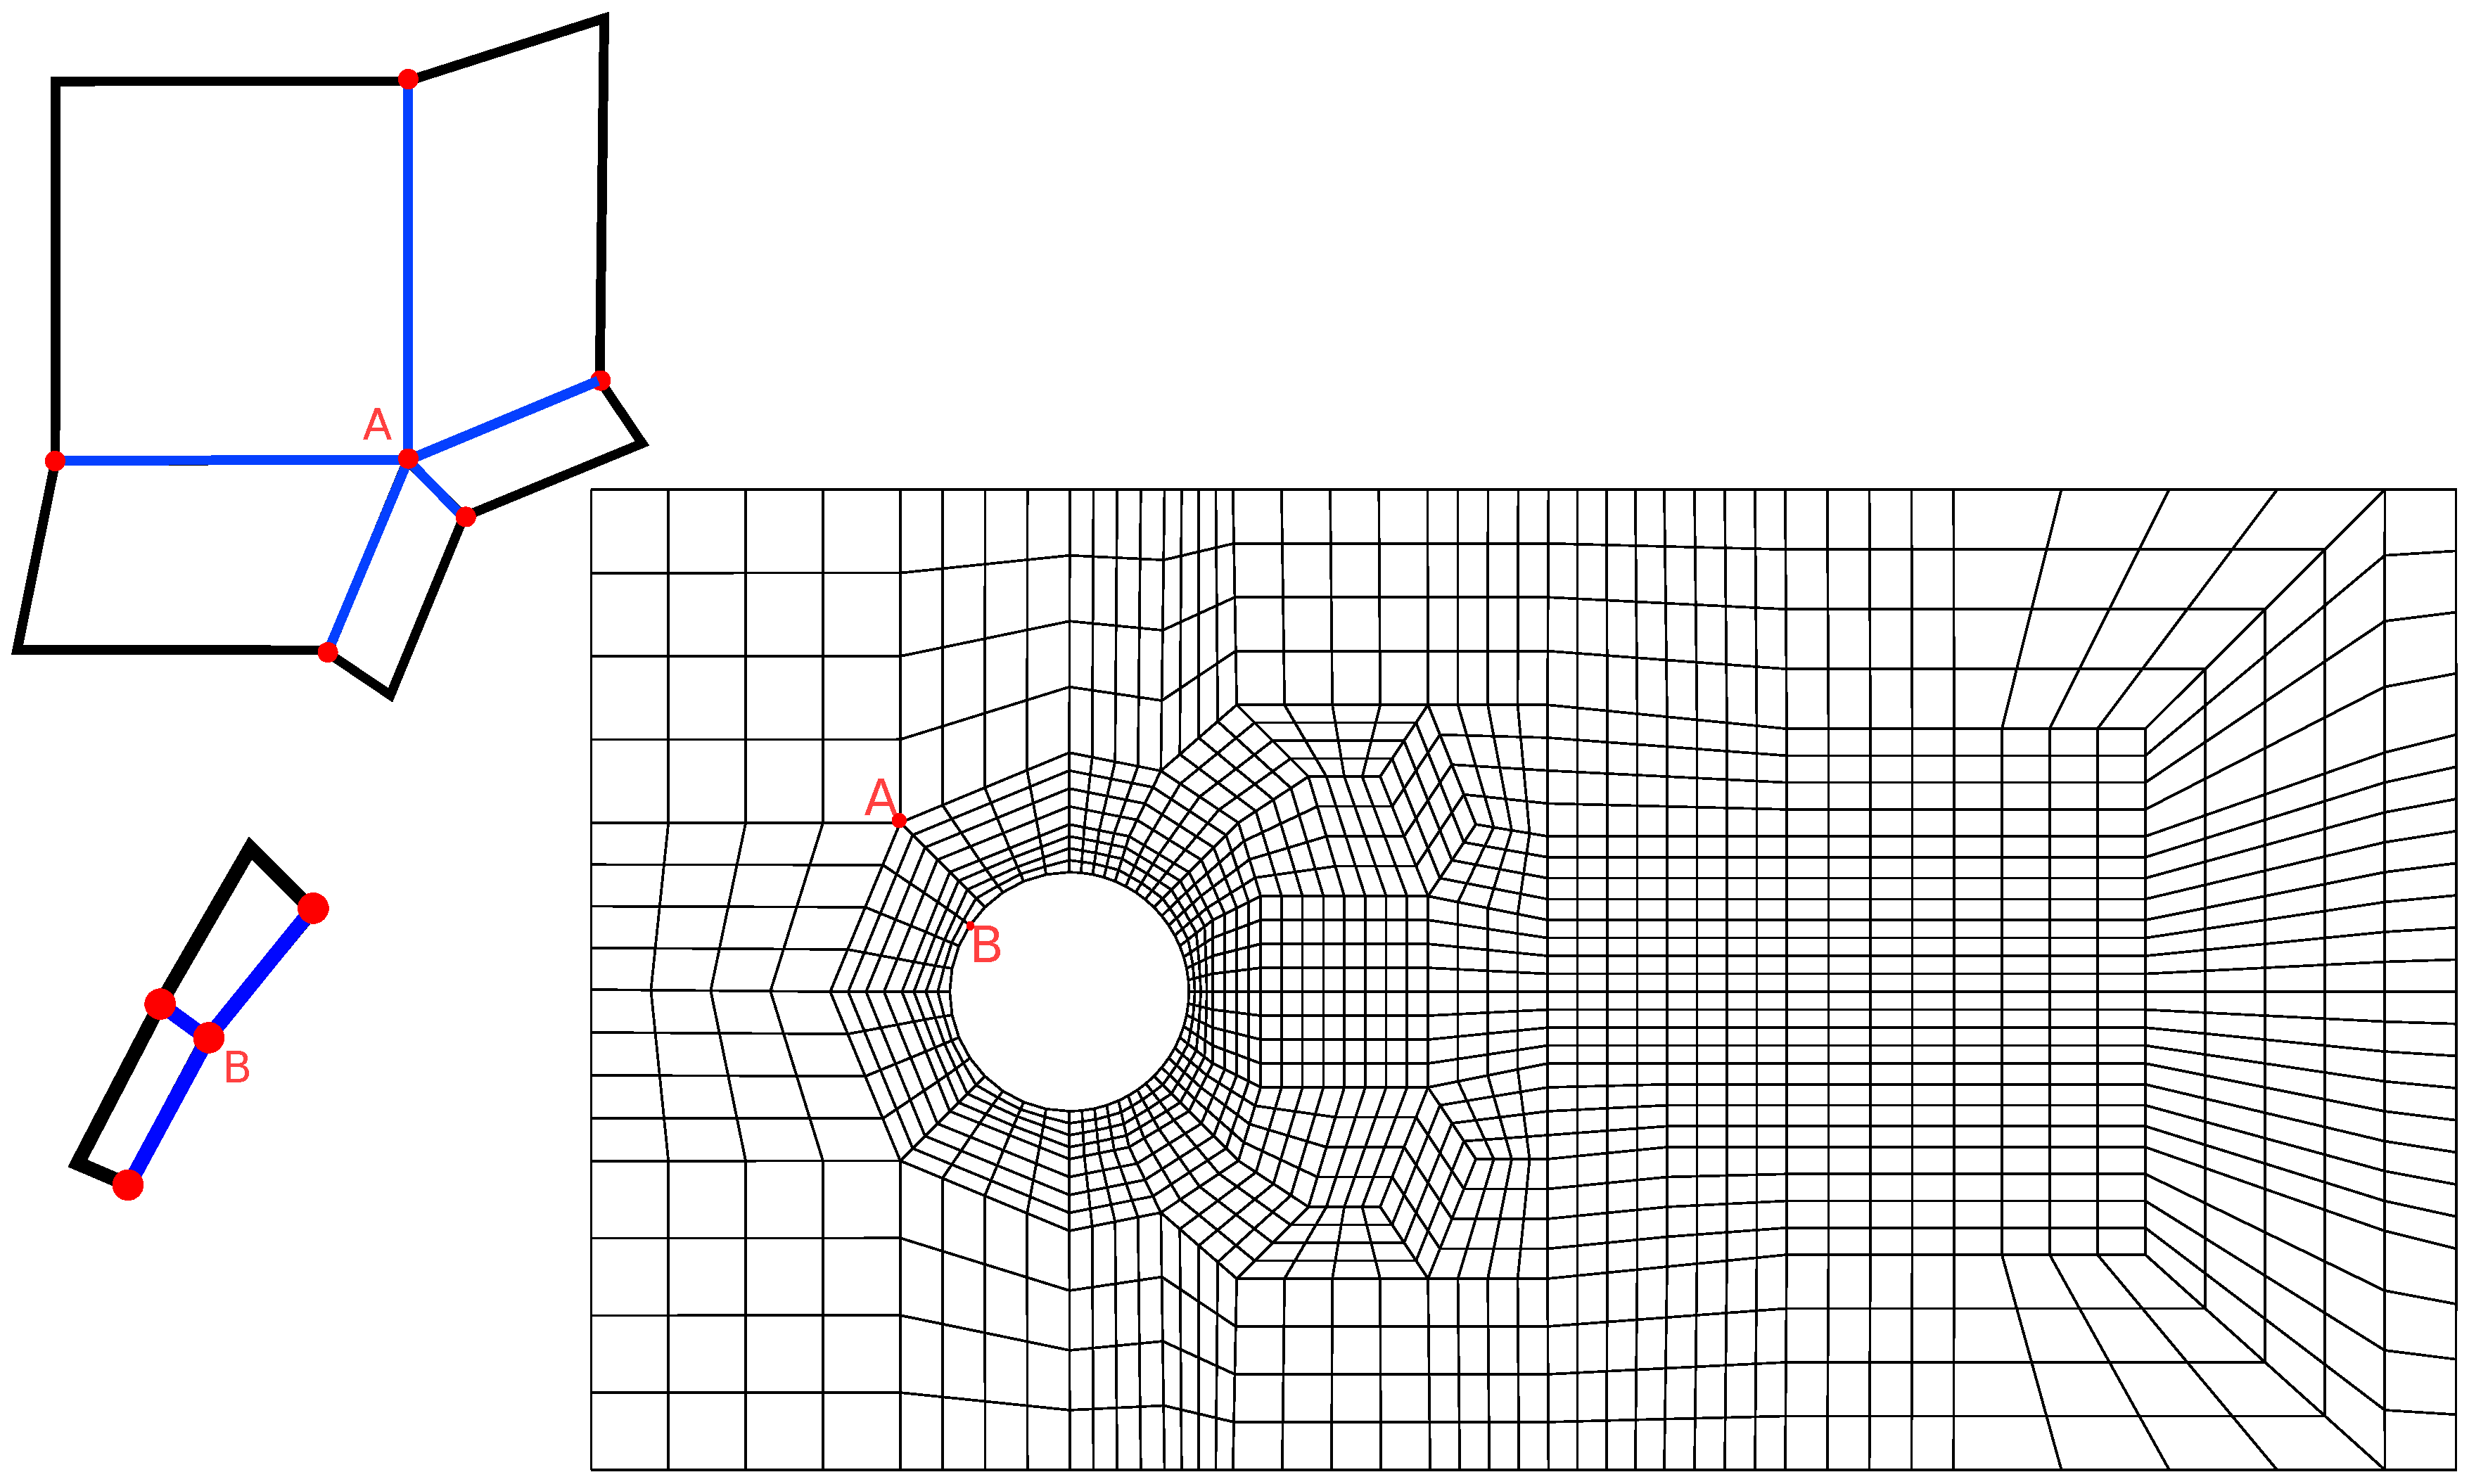
\includegraphics[width=0.7\textwidth]{Images/fac_unstructured.eps}
\end{center}
\caption{Unstructured 2D mesh where the mesh edges are aligned with an inner circle. We have marked some vertices with different 
degrees to that are used as anchor for connector elements (A) or as elements that approximate the circle geometry with its edges (B).}
\label{fig:unstructured-fac}
\end{figure}
\end{frame}

\begin{frame}
\begin{figure}[h!]
  \centering
  \subfloat[Mesh view with indicator function]{ 
    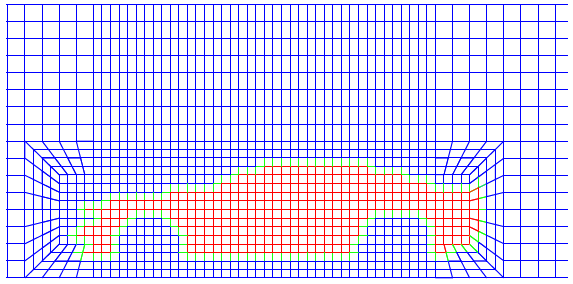
\includegraphics[width=0.5\textwidth]{Images/car-mesh.png}
    \label{fig:camaro-nondef}
  }
  \subfloat[Rendered surface mesh of the geometry]{ 
    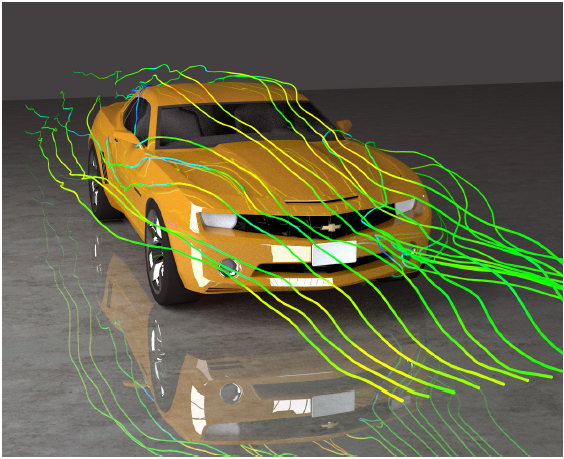
\includegraphics[width=0.5\textwidth]{Images/camaro.png}
    \label{fig:camaro}
  }
  \caption{Inside/outside indicator function}
  \label{fig:camaro-mesh}
\end{figure}
\end{frame}

\begin{frame}
\frametitle{Data Structures for Unstructured Meshes}
\begin{itemize}
\item Data structure needs to support hierarchical meshes/mesh levels $\rightarrow$ multi-grid solver
\item FEATFLOW based or derived software packages use the two-level ordering
\item Lowest Mesh level called the coarse grid
\item Mesh levels build successively, during refinement append vertices of next mesh level at the end of the vertex array
\item Thus indices in the connectivity information remain valid during refinement
\item Store connectivity arrays for each level individually
\end{itemize}
\end{frame}

\begin{frame}
\begin{figure}[h!]
\centering
\subfloat[The coarse mesh] {
\centering
 \includegraphics[width=0.35\textwidth]{Images/tc_base_mesh.eps}
 \label{fig:tc_base_mesh}
}
\hspace{1.0cm}
\subfloat[The fine mesh] {
\centering
 \includegraphics[width=0.35\textwidth]{Images/tc_mesh.eps}
 \label{fig:tc_mesh}
}
\caption{Pre-adapted hierachical mesh}
\label{fig:bench_setup}
\end{figure}
\end{frame}

\begin{frame}[fragile]
\frametitle{Unstructured Meshes Two-Level Ordering (FEATFLOW)}
\begin{itemize}
\item NVT: number of vertices on a level
\item NMT: number of edges on a level
\item NAT: number of faces on a level
\item NEL: number of faces on a level
\item During regular refinement we generate NMT+NAT+NEL new vertices
\item These are stored at the end of the current vertex array with the corresponding indices
\end{itemize}
Example of a 2D vertex array after a regular refinement. Before the refinement the length of the vertex array is NVT:
\begin{tikzpicture}
\matrix (A) [matrix of nodes,
                       every node/.style={text depth=.5ex,text height=2ex},
                       nodes={draw, minimum size=8mm, anchor=center}, 
											 nodes in empty cells, minimum height = 2cm,
											 row 2/.style={nodes={draw=none}},
											 row 3/.style={nodes={draw=none}},column sep=-\pgflinewidth,]											
    {		 
		 v & $\dots$ & v & e & $\dots$ & e & c & \dots & c\\
		$\uparrow$ & $\uparrow$ & $\uparrow$ & $\uparrow$ & $\uparrow$ & $\uparrow$ & $\uparrow$  & $\uparrow$ & $\uparrow$\\
		1 &  & nvt & nvt+1 &  & nvt+nmt & nvt+nmt+1 & & nvt+nel\\		
		};
%\foreach \i [evaluate=\i as \ni using {int(\i)}, evaluate=\i as \ntext using {int(\i)}] in {1,3,4,6} 
%    \draw [{Stealth}-, red!70] (A-1-\ni.south west)--++(-90:5mm) node[below] {\ntext};
\end{tikzpicture}
\end{frame}

\begin{frame}
\frametitle{Domain Decomposition}
\begin{figure}[h!]
\centering
\includegraphics[height=7cm]{Images/domains.eps}
\caption{Domain Decomposition in FEATFLOW: Whole domain (left), domain decomposed in 4 subdomains (right)}
\label{fig:domains}
\end{figure}
\end{frame}

\begin{frame}
\frametitle{Domain Decomposition for HPC}
\begin{itemize}
\item Solve the problem on the whole domain by computing a partial solution on each \keyword{subdomain}
\item The partial solutions on the subdomain are computed by different processing cores
\item \keyword{Domain Decomposition}: decompose or partition the domain into 'equal' subdomains
\item The amount of work that is assigned to each core should be as equal as possible
\item The amount of communication between cores/subdomains should be minimal
\item Software libraries for domain decomposition: 
\begin{itemize}
\item \keyword{Metis}: \url{http://glaros.dtc.umn.edu/gkhome/views/metis/}, FEATFLOW
\item \keyword{Scotch}: \url{https://www.labri.fr/perso/pelegrin/scotch/}, OpenFOAM
\end{itemize}
\end{itemize}
\end{frame}

\begin{frame}
\frametitle{Graph Theory and Domain Decomposition}
\begin{itemize}
%\item In the simulation workflow domain decomposition follows grid generation
\item Domain decomposition libraries such as Metis/Scotch use \keyword{Graph Theory} for decomposition
\item Meshes/Matrices can be represented as Graphs (i.e. Undirected Graph and Adjacency Matrix)
\item Graph Theory is also used for sparse matrix reordering 
\item The class of algorithms used in domain decomposition is \keyword{Graph Partitioning} algorithms
\item Graph partitioning algorithms can on their own be executed in parallel
\end{itemize}
\begin{figure}[h!]
\centering
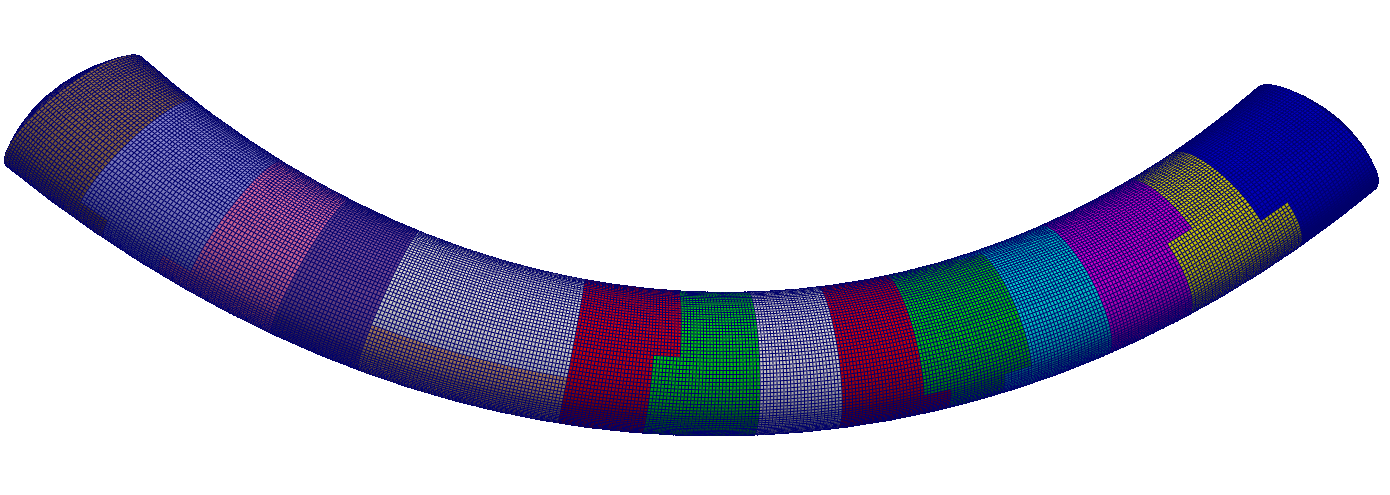
\includegraphics[height=5cm]{screenshots/domain-decomposition.png}
\label{fig:domains}
\end{figure}
\end{frame}

\begin{frame}
\frametitle{Mesh Adaptivity/Deformation}
\begin{itemize}
\item Accuracy of the simulation result increases with mesh resolution
\item Often a high accuracy solution is needed most in certain areas of interest
\item \keyword{Mesh adaptation} is used to increase mesh resolution without regular refinement
\item Different approaches to mesh adaptivity exist (some create \keyword{hanging nodes})
\item In \keyword{h-adaptivity} cells in a region of interest of the mesh are locally refined
\item The mesh connectivity is changed in the h-adaptivity approach
\item Hanging nodes can be a avoided by using connector elements
\item \keyword{r-adaptivity} moves existing nodes to increase resolution in regions of interest
\end{itemize}
\end{frame}

\begin{frame}
\begin{figure}[h!]
\centering
\subfloat[Adaptation to a circle by r-adaptivity] { 
 \includegraphics[width=10cm]{Images/fbm_r_adapt.eps}
}\\
\subfloat[Mesh adaptation to an airfoil by h-adaptivity] { 
 \includegraphics[width=10cm]{Images/h-adapt.eps}
}
\caption{Different types of mesh adaptation}
\end{figure}
\end{frame}

\begin{frame}
\frametitle{Local Refinement with Connector Elements}
\begin{figure}[h!]
\centering
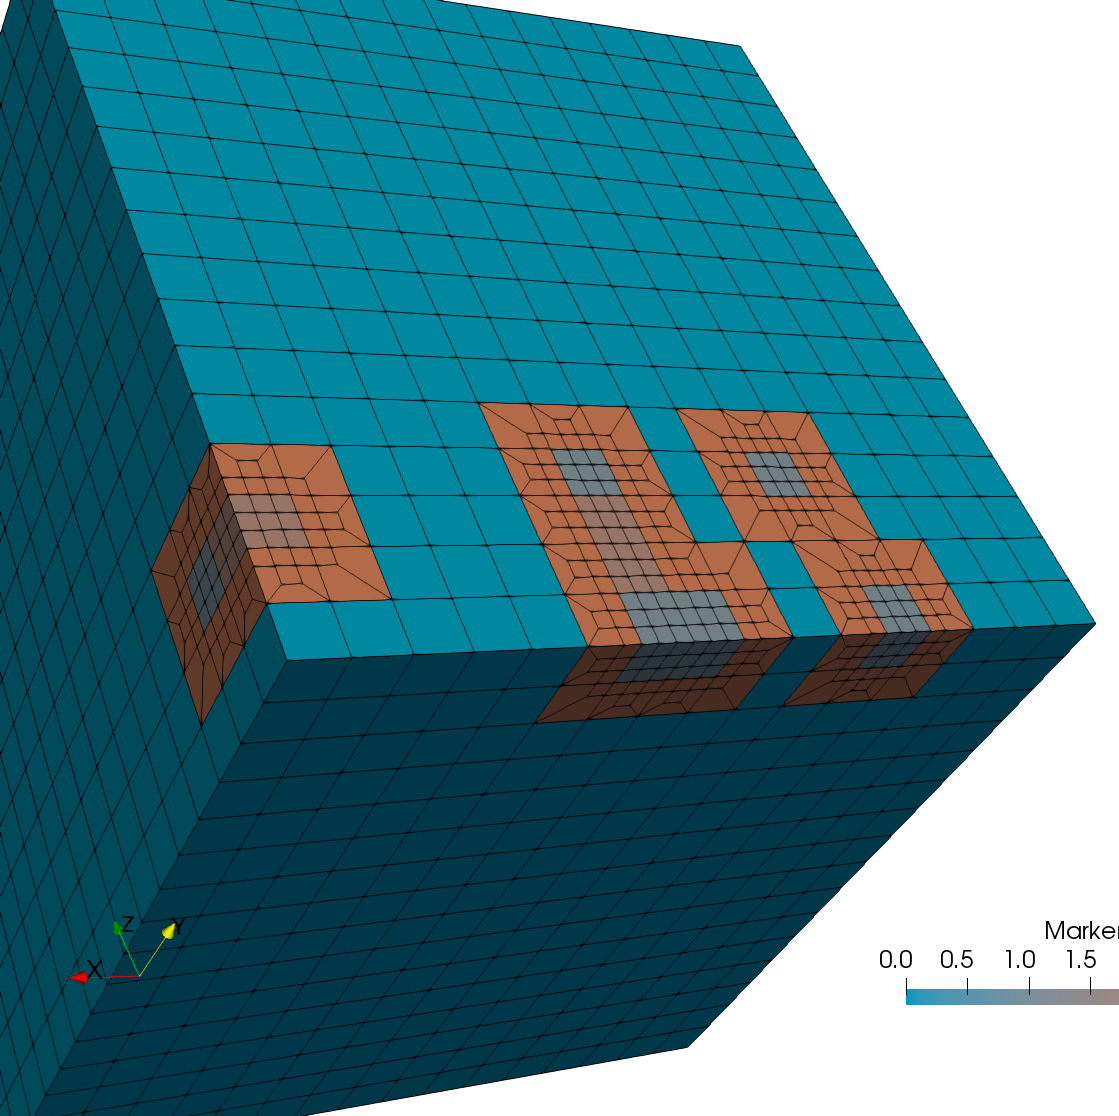
\includegraphics[width=0.48\textwidth]{screenshots/PROTOTYPE2.png}
\caption{Courtesy O.Mierka}
\label{fig:domains}
\end{figure}
\end{frame}

\begin{frame}
\begin{figure}[h!]
\centering
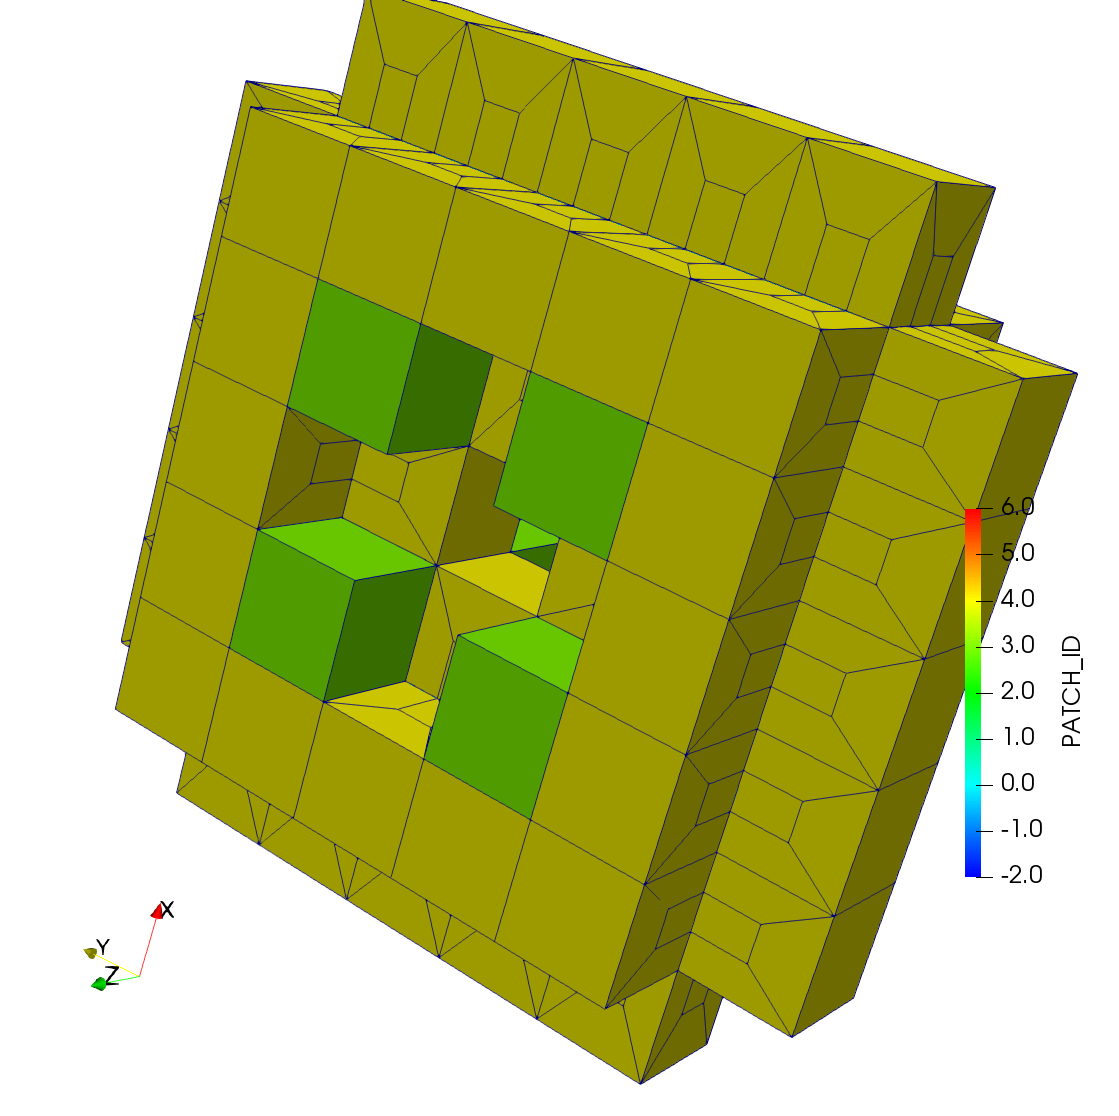
\includegraphics[width=0.5\textwidth]{screenshots/P4.png}
\label{fig:domains}
\caption{Courtesy O.Mierka}
\end{figure}
\end{frame}

\begin{frame}
\begin{figure}[h!]
\centering
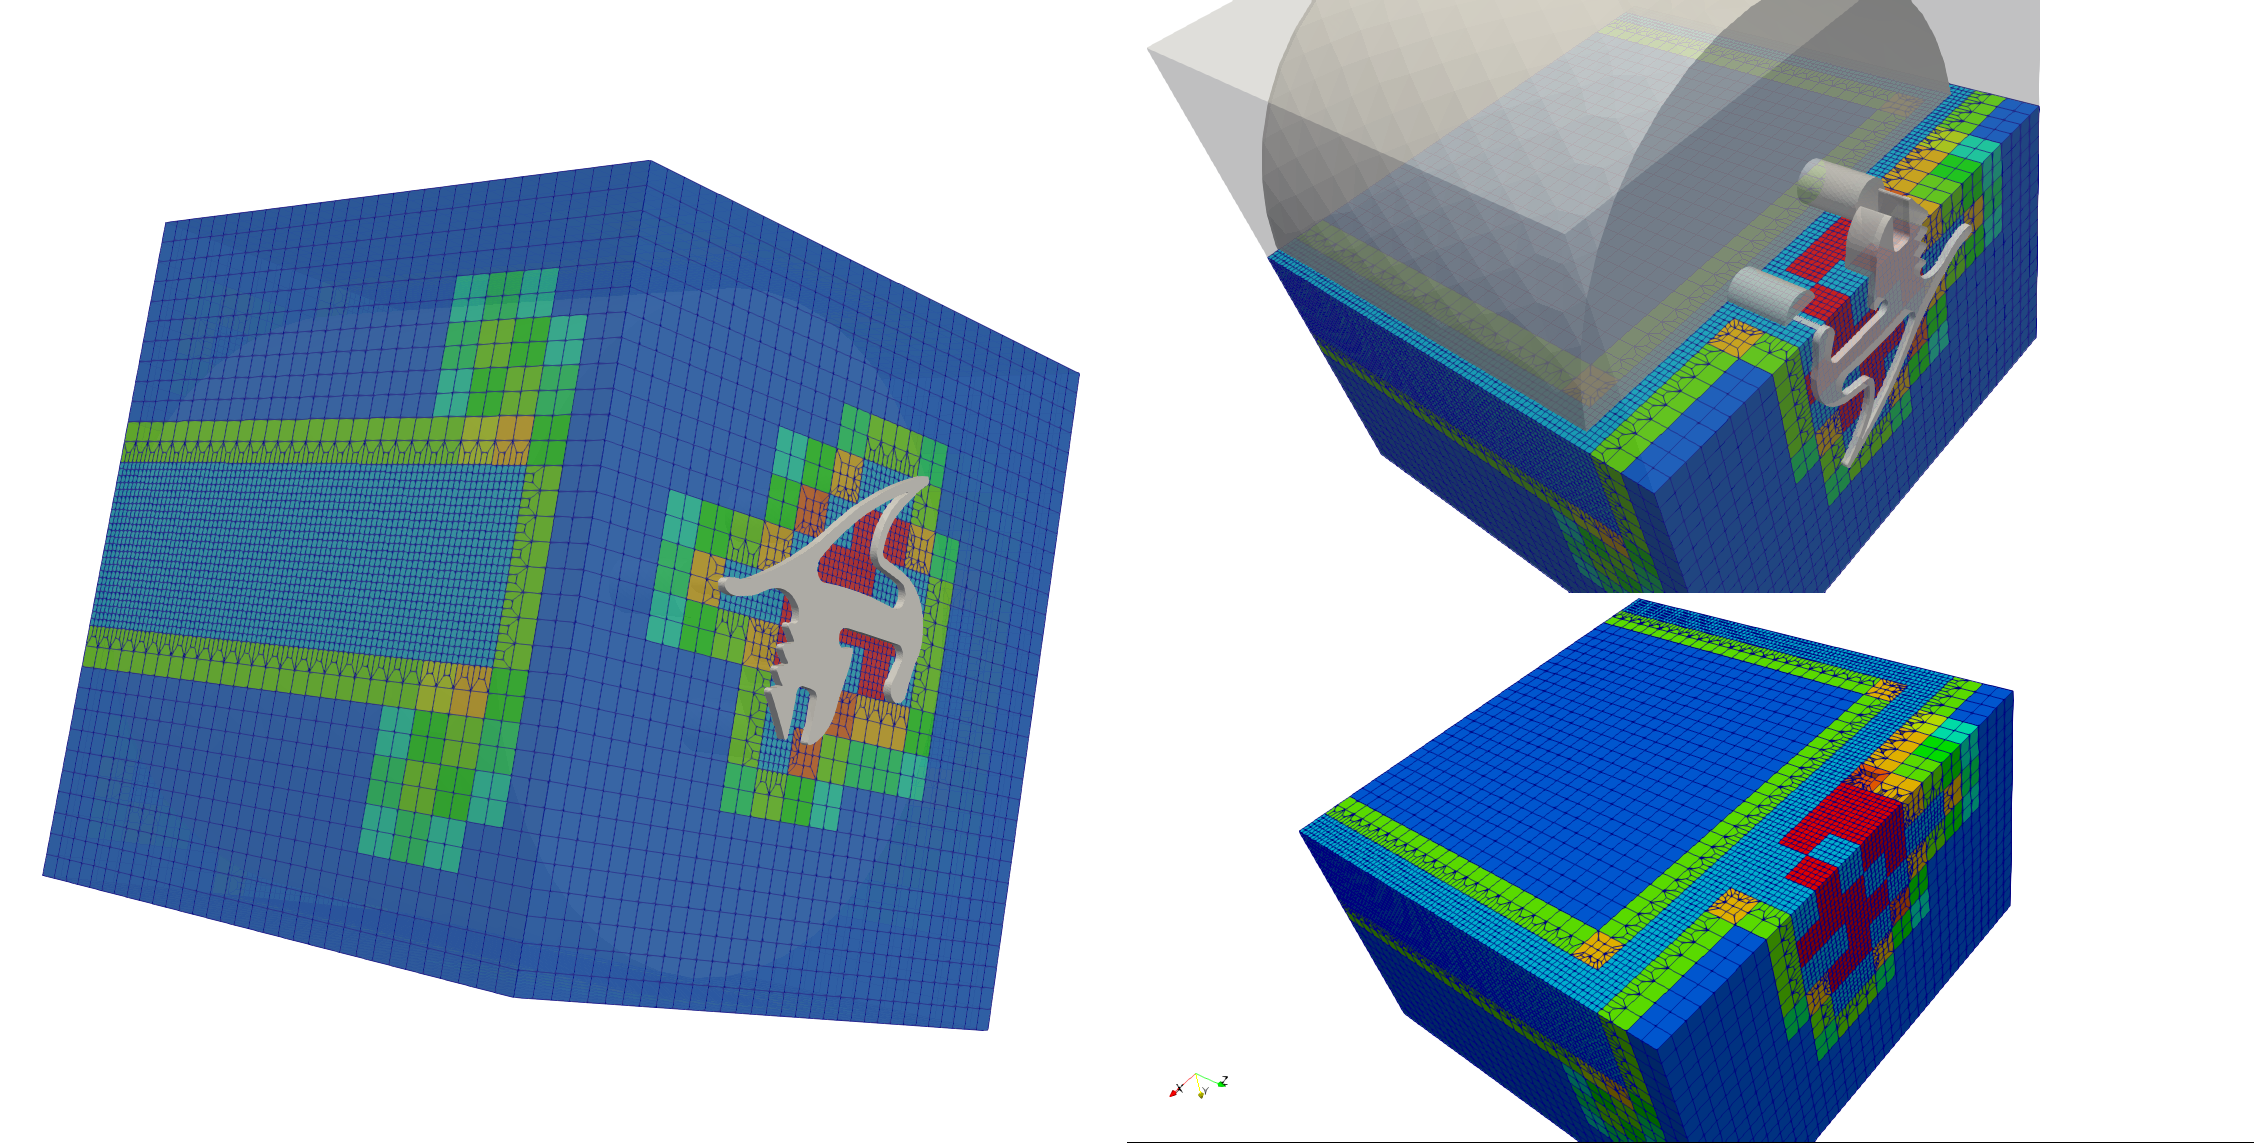
\includegraphics[width=1.\textwidth]{screenshots/GEO_BIW.png}
\label{fig:domains}
\caption{Courtesy O.Mierka}
\end{figure}
\end{frame}

\begin{frame}
\frametitle{R-Adaptivity}
\begin{itemize}
\item Moves existing nodes into region of interest without changing mesh connectivity
\item The r-adaptivity approach usually uses a \keyword{monitor function} to prescribe where nodes should be moved
\item The monitor function often uses distance calculations to move nodes that are already close to the region of interest
\item R-adaptivity can produce invalid elements (i.e. self-intersections) 
\item Iterative movement of nodes with smoothing passes can help prevent invalid elements
\item There exist PDE-based approaches \cite{GrajewskiKoesterTurek2008b} for r-adaptivity and algebraic methods based on \keyword{Laplacian Smoothing} \cite{Muenster:2016}
\end{itemize}
\end{frame}

\begin{frame}
\frametitle{Algebraic Mesh Adaptation using weighted Laplacian Smoothing}
\keyword{Laplacian smoothing} is usually used on meshes to reduce noise, it tries to rearrange nodes more to the center of its surrounding nodes. Laplacian smoothing in its smoother form is represented by the following equation:
\begin{equation*}
\mathbf{x}_{new} = (1-\omega) \cdot \mathbf{x} + \frac{\omega}{{\rm e}(\mathbf{x})} \cdot \sum\limits_{j=1}^{{\rm e}(\mathbf{x})} \mathbf{x}_j, 
\label{eq:laplace-smoother}
\end{equation*}
We can introduce vertex weights in order to move vertices closer to the region of interest, be giving vertices in that region a higher weight:
\begin{equation*}
\mathbf{x}_{i}^{\rm new} = (1-\omega) \cdot \mathbf{x}_{i}^{\rm old} + \omega \cdot \frac{\sum\limits_{j=1,n}^{{{\rm e}(i)}} w_j \mathbf{x}_j^{\rm old}}{\sum\limits_{j=1}^{{\rm e}(i)} w_j}\quad {\rm for} \quad i=1,n
\end{equation*}
\end{frame}

\begin{frame}
\begin{figure}[h!]
\centering
\subfloat[The weights for the laplace smoother are generated by combining the signed distance $d(\mathbf{x})$ with a hat function] { 
 \includegraphics[width=10cm]{Images/monitor_func.eps}
 \label{fig:mon}
}\hspace{0.1cm}
\subfloat[Visualization of $w(\mathbf{x})$ on the undeformed mesh] {
  \raisebox{3.5\baselineskip}{
 \includegraphics[width=10cm]{Images/mon}
 \label{fig:mon_field}
 }
}
\caption{Generation of the weight distribution function $w(\mathbf{x})$}
\label{fig:monitor_func}
\end{figure}

\end{frame}

\begin{frame}[plain]
\begin{figure}[h!]
  \centering
  \subfloat[Cylinder appears round in a two-color map]{ 
    \includegraphics[width=13.0cm]{Images/fbm_laplace_con.eps}
  }\\
  \subfloat[The mesh nodes are concentrated near the surface of the cylinder]{ 
    \includegraphics[width=13.0cm]{Images/fbm_laplace_con_edges.eps}
  }
  \caption{Cylinder resolution for the Laplace-$\kappa$ adaptation}
  \label{fig:osc-cyl-lap-kappa}
\end{figure}
\end{frame}

\begin{frame}[plain]
\begin{figure}[h!]
  \begin{center}
    \includegraphics[width=1.0\textwidth]{Images/drag_coefficient_laplace_kappa_classic_fbm.eps}
    \caption{Drag curves for the standard FBM, Laplace-$\alpha$ and Laplace-$\kappa$ calculations}
    \label{fig:drag-kappa-classic}
  \end{center}
\end{figure}
\end{frame}

\begin{frame}[plain]
\begin{figure}[h!]
  \begin{center}
    \includegraphics[width=1.0\textwidth]{Images/lift_kappa_fbm.eps}
    \caption{Drag curves for the standard FBM, Laplace-$\alpha$ and Laplace-$\kappa$ calculations}
    \label{fig:lift-kappa-classic}
  \end{center}
\end{figure}
\end{frame}

\begin{frame}
\frametitle{Mesh Generator Salome}
\begin{itemize}
\item \url{https://www.salome-platform.org/}
\item Full-featured open-source CAD + mesh generator 
\item Integrates many open-source meshing libraries by plug-ins (i.e. netgen)
\item Allows a user to design geometries with semantic parts (inflow, outflow, walls, ...)
\item Calculate quality metrics on meshes
\item Many different mesh format available (i.e., export to OpenFOAM)
\item Possible to execute tasks in batch mode by Python scripts
\item Geared towards students, good documentation and example projects
\end{itemize}
\end{frame}


%\begin{frame}
	\frametitle{About ParaView}

      \begin{block}{ParaView Features}
        \begin{itemize}
		\item Open-source and multi-platfrom visualization software
		\item Visualization backend provided by VTK library
		\item Huge number of visualization filters  
                \item Extension is possible by programmable filters (Python) or 
                \item User defined plugins  
		\item Import and export of data to various formats used in CFD packages
		\item Easy access to numerical data for internal or external plotting etc.
		\item Tasks can be automated by using the PvPython interface
		\item Client/Server paradigm to view Big Data on remote clusters
        \end{itemize}
      \end{block}

\end{frame}

\begin{frame}
  \frametitle{How To Obtain ParaView}
    \begin{itemize}
      \item Current Stable Version: 5.8.1
      \item Current Release Candidate: 5.9.0-RC2			
      \item ParaView/KitWare website: https://www.paraview.org
			\item Download: https://www.paraview.org/download/
      \begin{itemize}			
				\item Windows
				\item Linux-Variants
				\item macOS
      \end{itemize}			
    \end{itemize}
    \begin{center}
      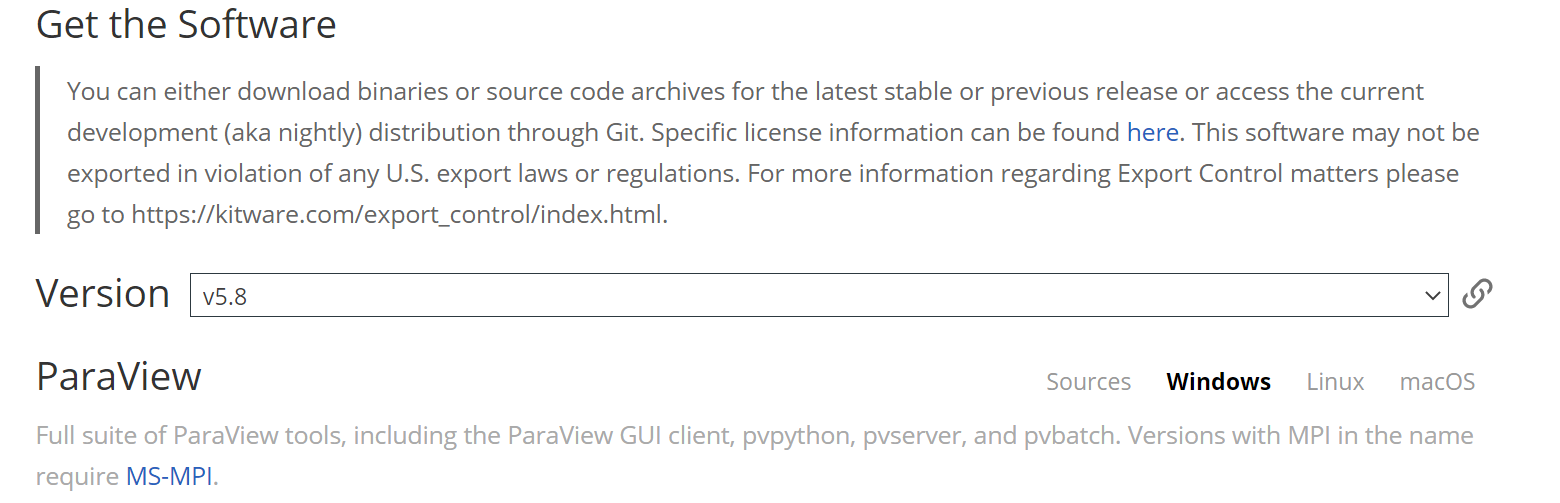
\includegraphics[width=0.6\textwidth]{screenshots/download-pv.png}
    \end{center}		
\end{frame}

\begin{frame}
  \frametitle{ParaView Software Ecosystem}
  \vspace{-0.9cm}
  \begin{tikzpicture}[remember picture,overlay]
    \tikzset{shift={(current page.center)},yshift=-1.5cm}

    \node[text width=8cm] (C1) at (-8, -0.0) {
      \begin{block}{VTK}
        \begin{itemize}
          \item Visualization backend
          \item Uses OpenGL
        \end{itemize}
      \end{block}
    };

    \node[text width=8cm] (C2) at (8,-0.7) {
      \begin{block}{Qt (cute)}
        \begin{itemize}
          \item Provides widges and other GUI controls
          \item Support for modular plugins
        \end{itemize}
      \end{block}
    };

    \node[text width=8cm] (C3) at (0,4) {
      \begin{block}{CMake}
        \begin{itemize}
          \item Script language to control the building process
          \item Generates a wide range of specific build files
        \end{itemize}
      \end{block}
    };

    \node[text width=8cm] (C4) at (0,-4.85) {
      \begin{block}{ParaView}
        \begin{itemize}
          \item VTK visualization by GUI
          \item Scripting via Python
          \item Extension by plugins
        \end{itemize}
      \end{block}
    };

\end{tikzpicture}
\end{frame}


\begin{frame}
  \frametitle{Use Cases of Visualization Software}

      \begin{block}{Typical ParaView Use Cases}
        \begin{itemize}
          \item Provide an intuitive illustration of raw simulation data

          \item Highlight key features of specific flow features

          \item Provide an intuitive understanding for non-expert viewers  

          \item Help in the testing/debugging process of CFD software 

          \item Assist during result validation by providing analysis tools  

          \item Convert data in different formats in order to communicate with collaborators
        \end{itemize}
      \end{block}

\end{frame}

\begin{frame}
  \frametitle{ParaView Interface}

  \begin{tikzpicture}[remember picture,overlay]
    \tikzset{shift={(current page.center)},yshift=-1.5cm}

    \node[align=center,scale=0.3,transform shape] (C1) at (0,0)
    {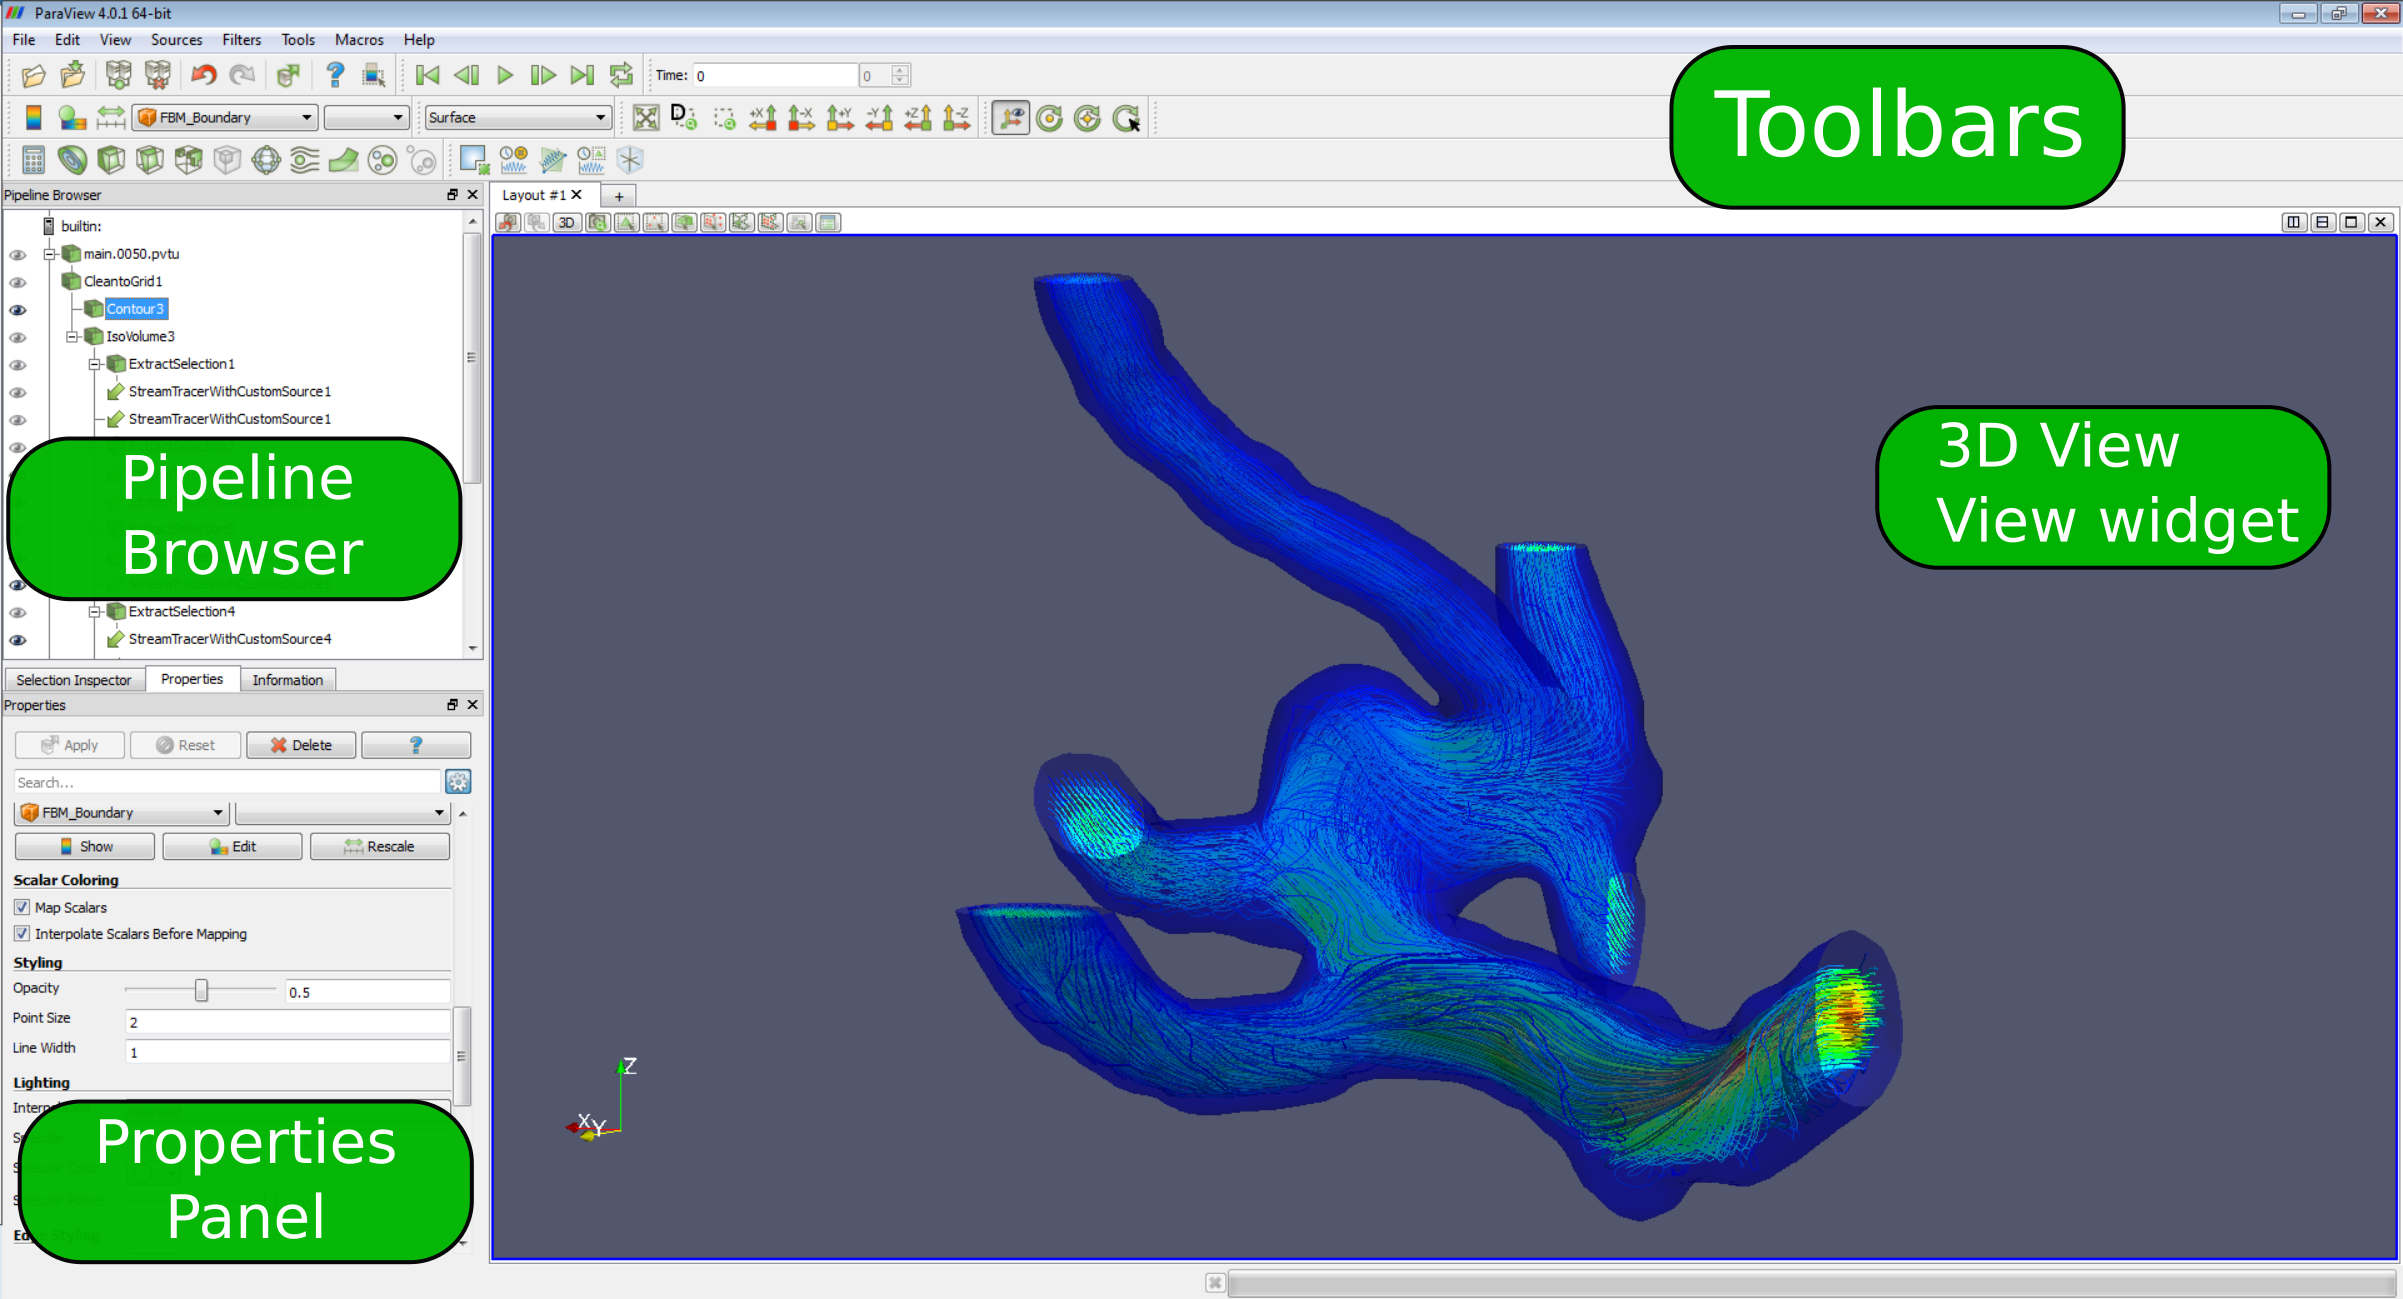
\includegraphics{screenshots/pv-gui.png}};

\end{tikzpicture}

\end{frame}

\begin{frame}[fragile]
  \frametitle{Filter Pipeline Concept}

    \begin{minipage}{0.45 \textwidth}

      \begin{tikzpicture}%[nodes=draw]

    \node[text width=8cm] (C1) at (-8, 1.25) {
      \begin{block}{Filter Pipeline}
        \begin{itemize}
          \item A \keyword{filter} is an operation on an input data set
          \item Filters can be chained (pipelined)  
          \item More complex visualizations require multiple filters 
        \end{itemize}
      \end{block}
    };

    \node[align=center,scale=0.5,transform shape] (C1) at (-10,-5.0)
    {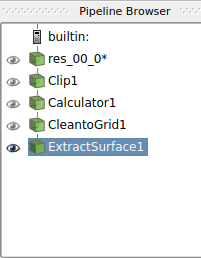
\includegraphics{screenshots/filters.png}};

    \end{tikzpicture}

    \end{minipage}
    \begin{minipage}{0.45 \textwidth}
      \begin{center}
        \begin{tikzpicture}%[nodes=draw]

          \node[align=center,scale=0.189,transform shape] (C1) at (10,-1)
          {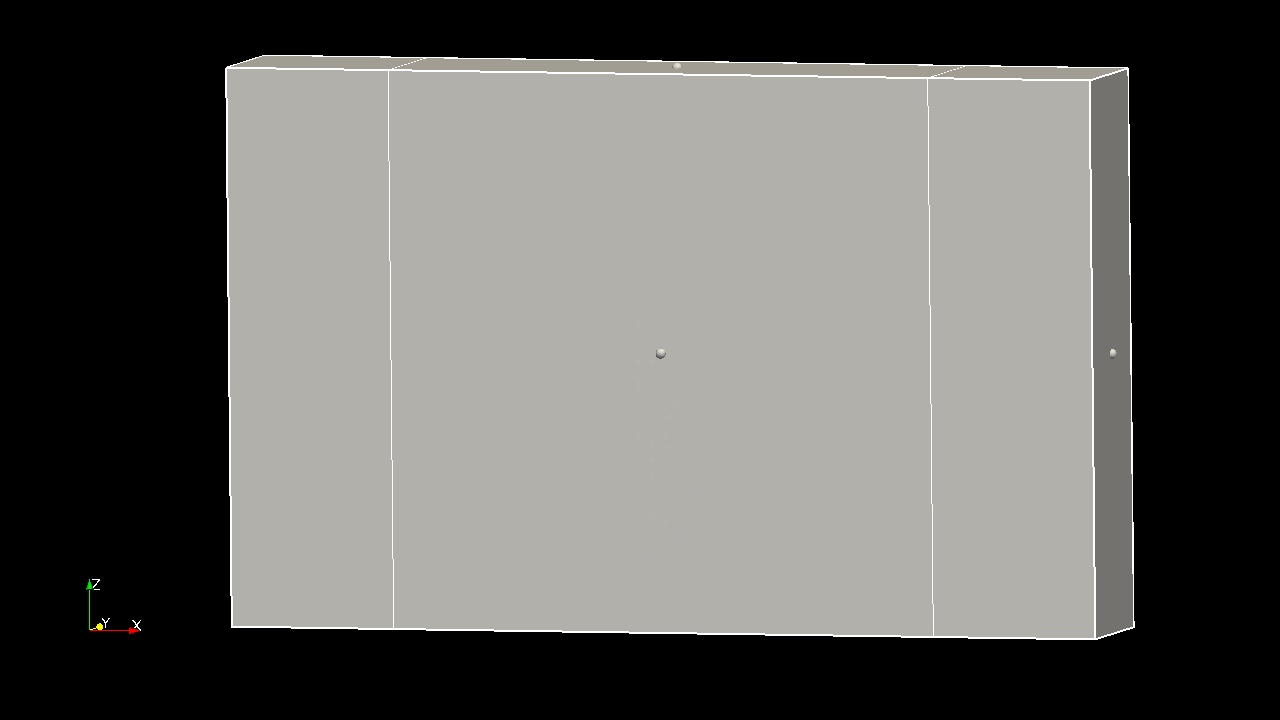
\includegraphics{screenshots/begin-filter.png}};

            \node [scale=2.8,
            fill=TUgreen, 
            single arrow,
            rotate=270, 
            font=\sffamily
            ] at (10.0,-4.22)  
            {\rotatebox{270}{}};

          \node[align=center,scale=0.8,transform shape] (C2) at (10,-8)
          {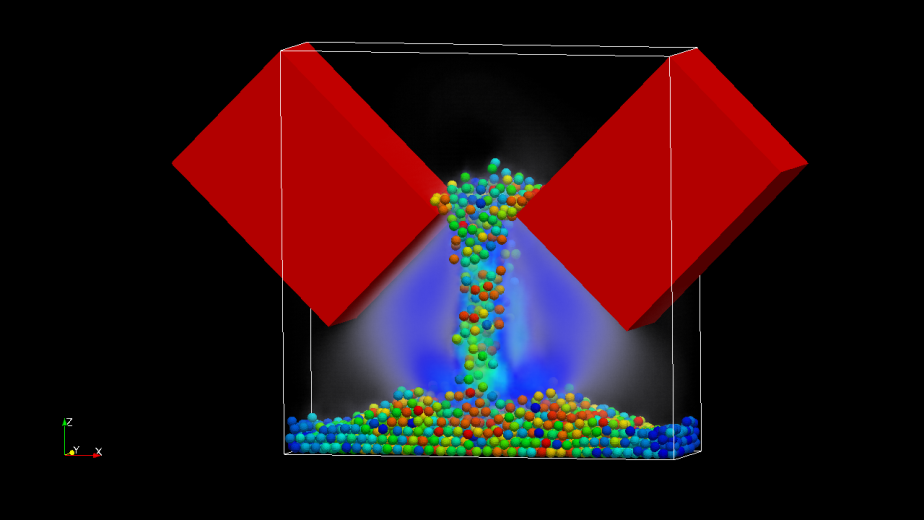
\includegraphics{screenshots/end-filter.png}};

        \end{tikzpicture}
      \end{center}
    \end{minipage}
\end{frame}

\begin{frame}[plain]
  \vspace{3cm}
  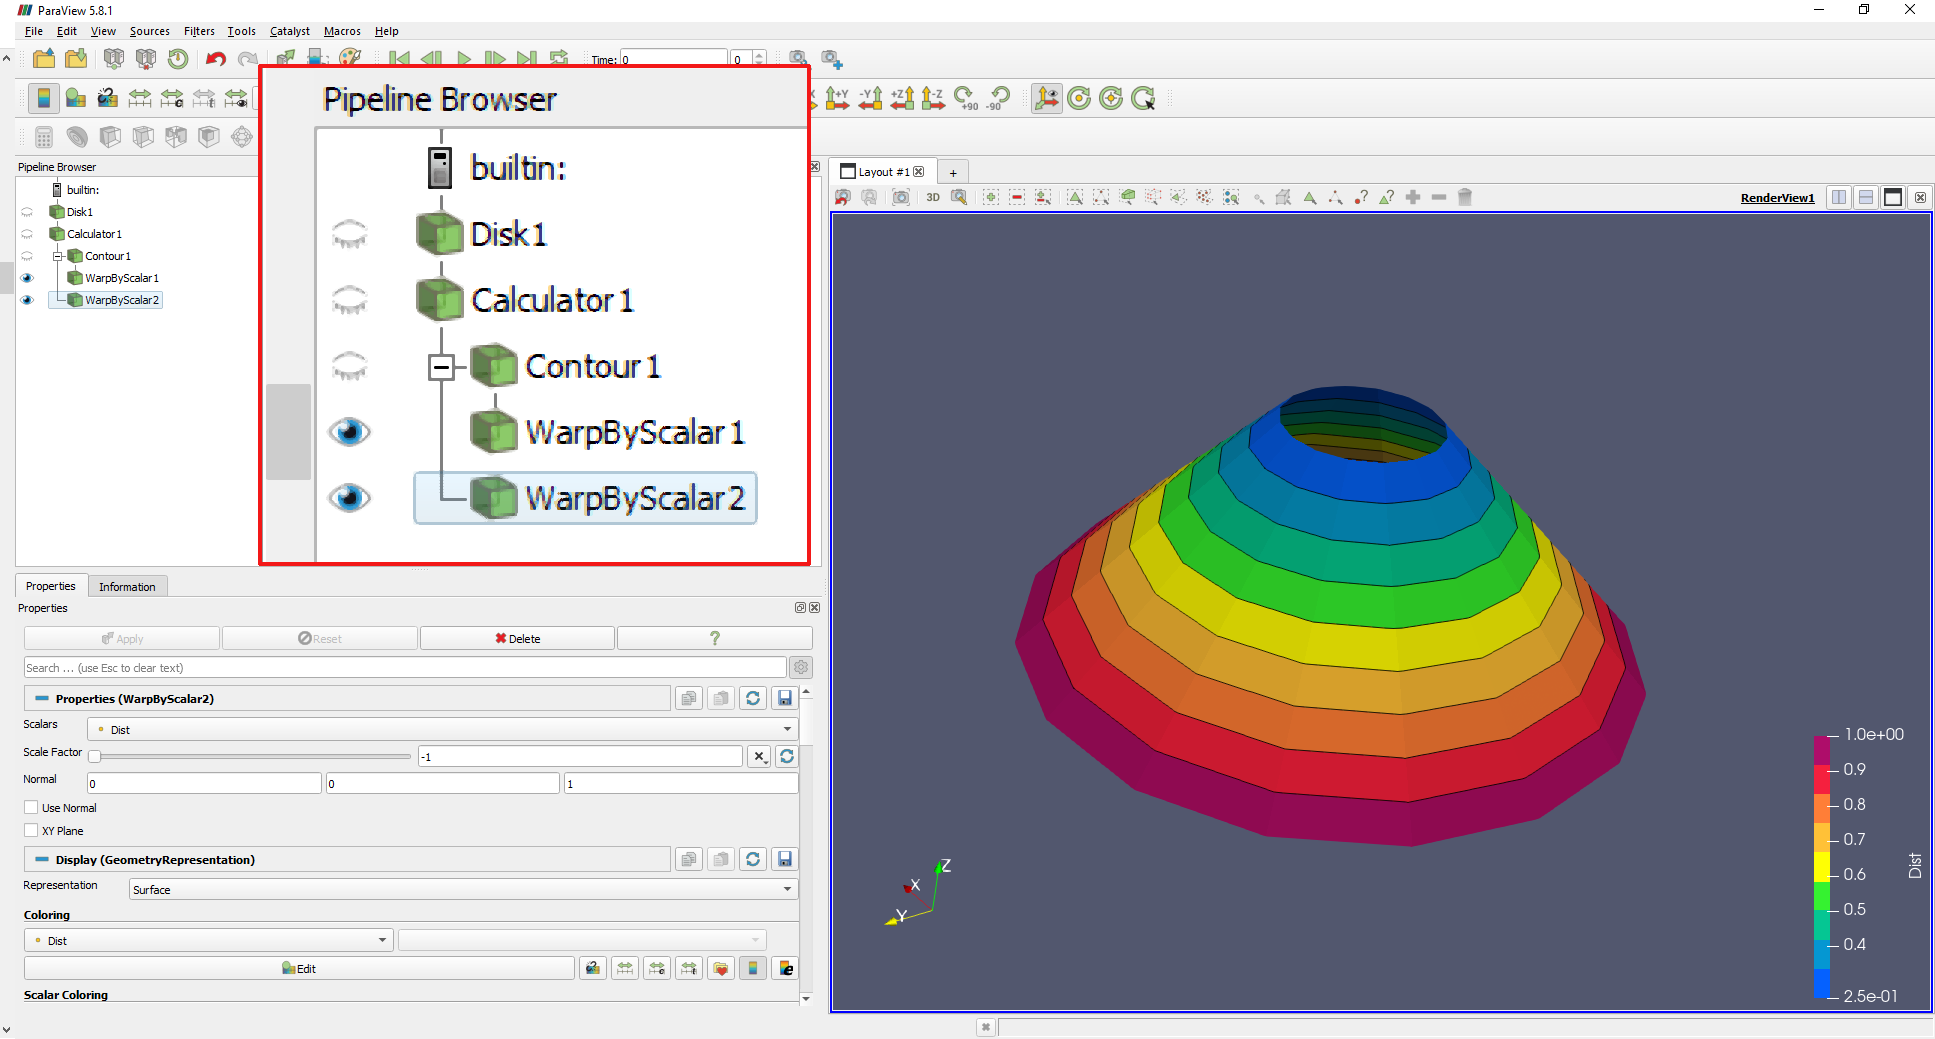
\includegraphics[width=0.95\textwidth]{screenshots/pipeline0.png}
\end{frame}

\begin{frame}
  \frametitle{Applying and Configuring a (Slice) Filter}
	\begin{center}
	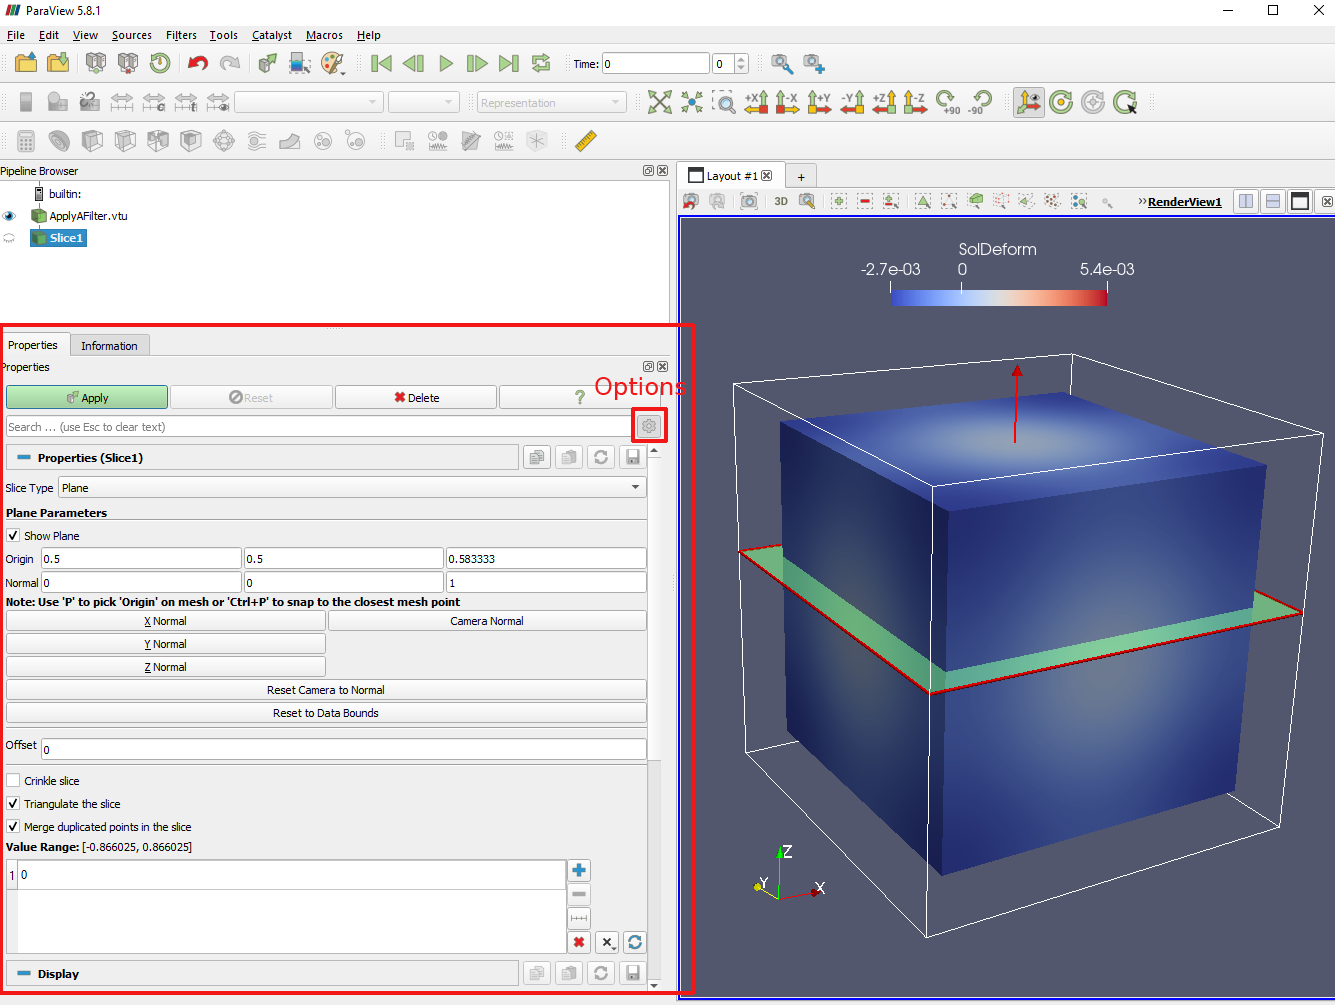
\includegraphics[width=0.7\textwidth]{screenshots/filter-apply.png}		
	\end{center}
\end{frame}

\begin{frame}
  \frametitle{Applying and Configuring a (Slice) Filter II}
    \begin{itemize}
      \item \keyword{Control widgets} in the viewport to manually/visually configure filters
      \item In the \keyword{Properties Panel} the filter can be configured with numbers
      \item The \keyword{Gear Icon} can open/close additional configuration options			
      \item The \keyword{Apply Button} is used to apply the current configuration of the filter						
      \item When the configuration is changed it needs to be reapplied $\mapsto$ \keyword{Apply Button}
			\item Filter configurations can be copied to quickly apply the same configuration multiple times
    \end{itemize}
\end{frame}
  
\begin{frame}
  \frametitle{View Properties Panel}
    \begin{itemize}
      \item Change general visualization and rendering properties/options
      \item Change \keyword{Opacity/Transparency} to make it possible to see through certain objects
      \item Change rendering properties for objects to give them a special appearence
      \item Change solid color, color maps or color of edges
      \item Change the projection method between \keyword{parallel} and \keyword{perspective} (useful for selections)
      \item Increase/decrease rendering quality of source objects
      \item Display \keyword{grid axes} around an object
    \end{itemize}
\end{frame}

\begin{frame}
  \frametitle{View Properties Panel II}
  \begin{center}
    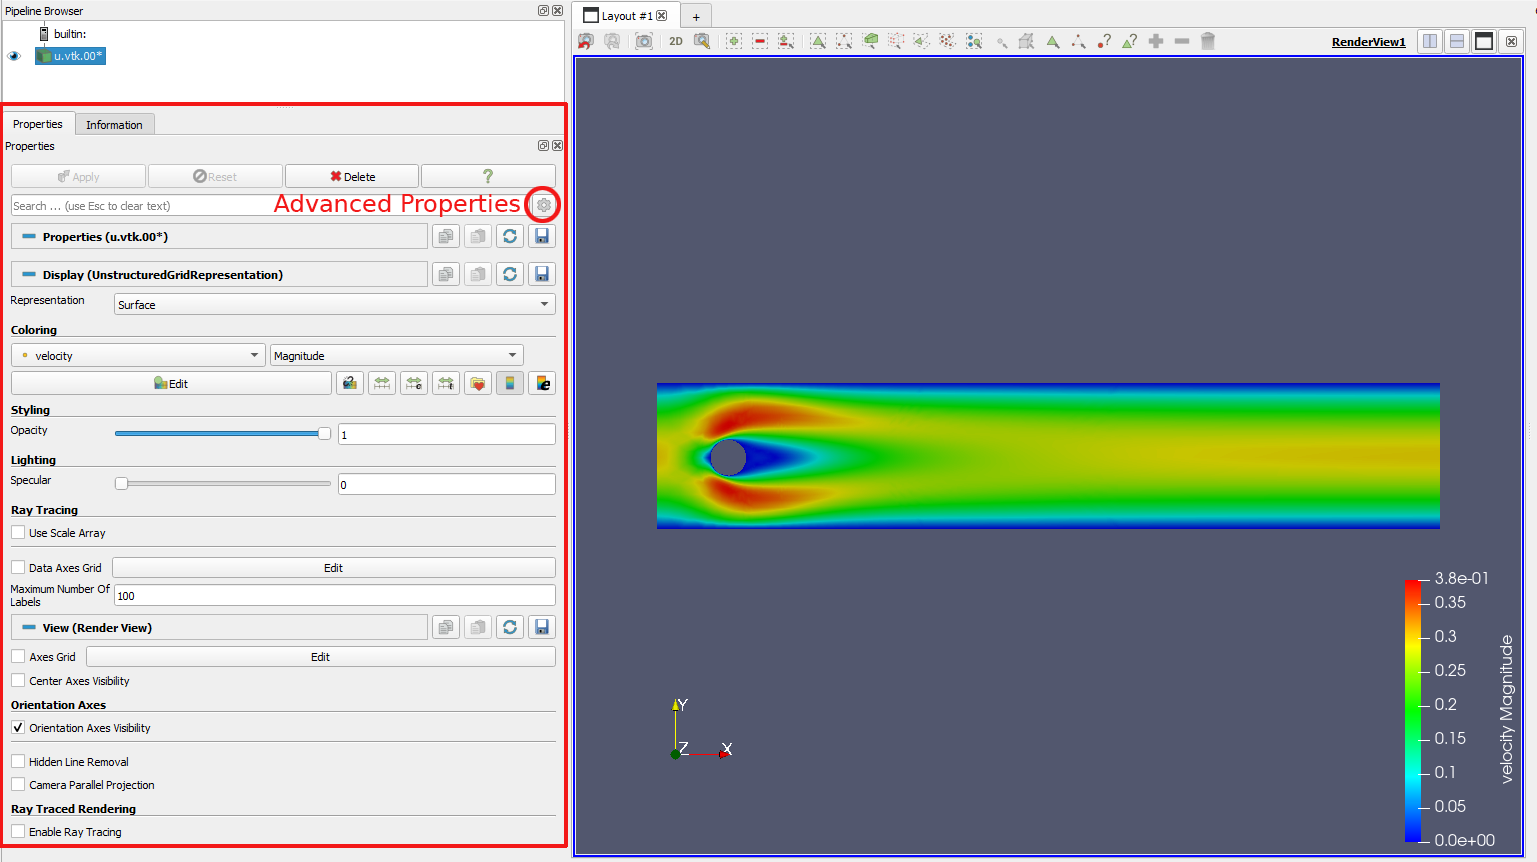
\includegraphics[width=0.9\textwidth]{screenshots/properties-1.png}
  \end{center}
\end{frame}

\begin{frame}
  \frametitle{Camera and Axes Toolbar}

  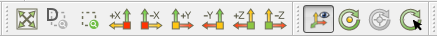
\includegraphics[width=\textwidth]{screenshots/camerabar.png}

    \begin{itemize}
      \item Reset the camera to its default parameters
      \item Magnify a rectangular selection of the view area
      \item Choose a certain coordinate axes plane to look at
      \item Toggle rendering of orientation axes 
      \item Toggle rendering of center of rotation 
      \item Select a new center of rotation 
    \end{itemize}
\end{frame}

\begin{frame}
  \frametitle{Basic Filters}

    \begin{itemize}
      \item \keyword{Slice}: Extract a plane, box-, sphere- or cylinder surface out of a data set
      \item \keyword{Clip}: Extract a plane, box-, sphere- or cylinder volume out of a data set
      \item \keyword{Warp by Scalar}: Visualizes a scalar value by a height extrusion on a 2D data set 
      \item \keyword{Contours}: Increases visibility of different solution contour levels 
      \item \keyword{Surface LIC}: Streamlines on pixel basis, highlights small scale flow features 
      \item \keyword{Glyphs}: Streamlines on pixel basis, highlights small scale flow features 

      \item \keyword{Stream Traces}: Visualizes the pathline of a particle through a \emph{stationary} vector field 
    \end{itemize}

\end{frame}

\begin{frame}
  \frametitle{Color Maps}
    \begin{itemize}
      \item Choose a color gradient map for your data set
      \item Create your own color map from scratch or by modifying an existing
      \item Popular choice for CFD: \keyword{Blue to Red Rainbow Gradient}
      \item Customize the number of discrete colors in the color map (contour visualization)
      \item Customize the mapping of colors to numerical values in the data set
      \item Set your customized settings as defaults
    \end{itemize}
		\vspace{2cm}
  \begin{center}
    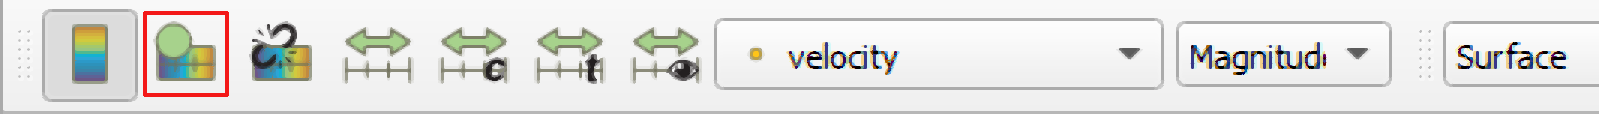
\includegraphics[width=0.9\textwidth]{screenshots/color-map-icon.png}
  \end{center}
\end{frame}

\begin{frame}
\vspace{-1cm}
  \begin{center}
    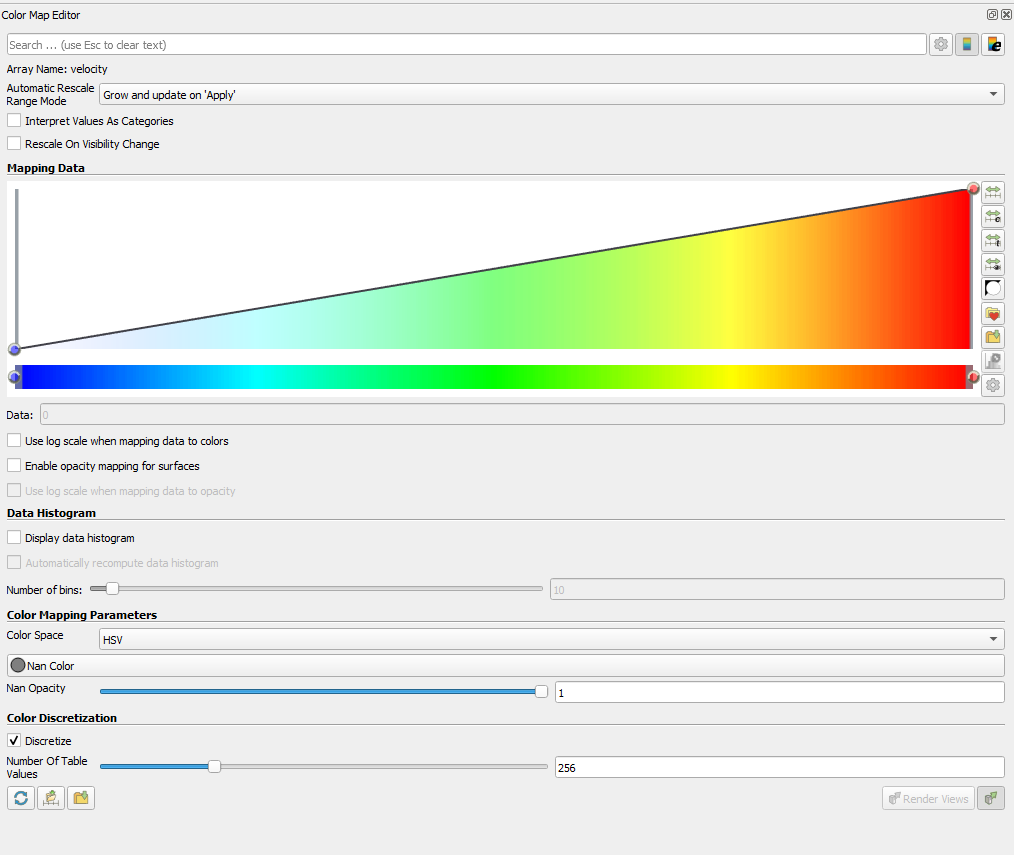
\includegraphics[width=0.8\textwidth]{screenshots/color-map-editor.png}
  \end{center}
\end{frame}

\begin{frame}
  \frametitle{Color Palette}
    \begin{itemize}
      \item Change the default color configuration of ParaView
      \item Set new colors for edges, surfaces, selection, background
      \item Quickly switch color configurations to highlight certain features of your data
      \item Change the color configuration for screenshots (often require white background)
      \item Save your custom configuration and import or export it
    \end{itemize}
  \begin{center}
    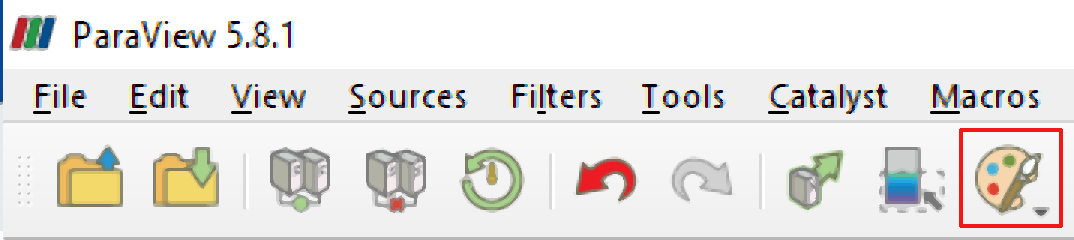
\includegraphics[width=0.9\textwidth]{screenshots/color-palette-icon.png}
  \end{center}
\end{frame}

\begin{frame}
  \frametitle{State Files}

    \begin{itemize}
      \item \keyword{State file}: XML format based file with the ending .pvsm that is used to store the currently applied filters and a reference to the currently loaded data sets to a file
      \item Used to quickly restore a state or to recover from a crash
      \item The reference to the data set can be changed upon loading the state file in order to apply the
        filters to a different data set or if the location of the data on the hard drive has changed
      \item This way state files can be used to exchange a ParaView visualization with collaborators, they only need to set the location of their data set upon loading the state file
      \item State files can be exchanged between different version of ParaView
      \item Accessible from Menu: \keyword{File->Load State...}
    \end{itemize}
        

\end{frame}

\begin{frame}[plain]
  \vspace{3cm}
  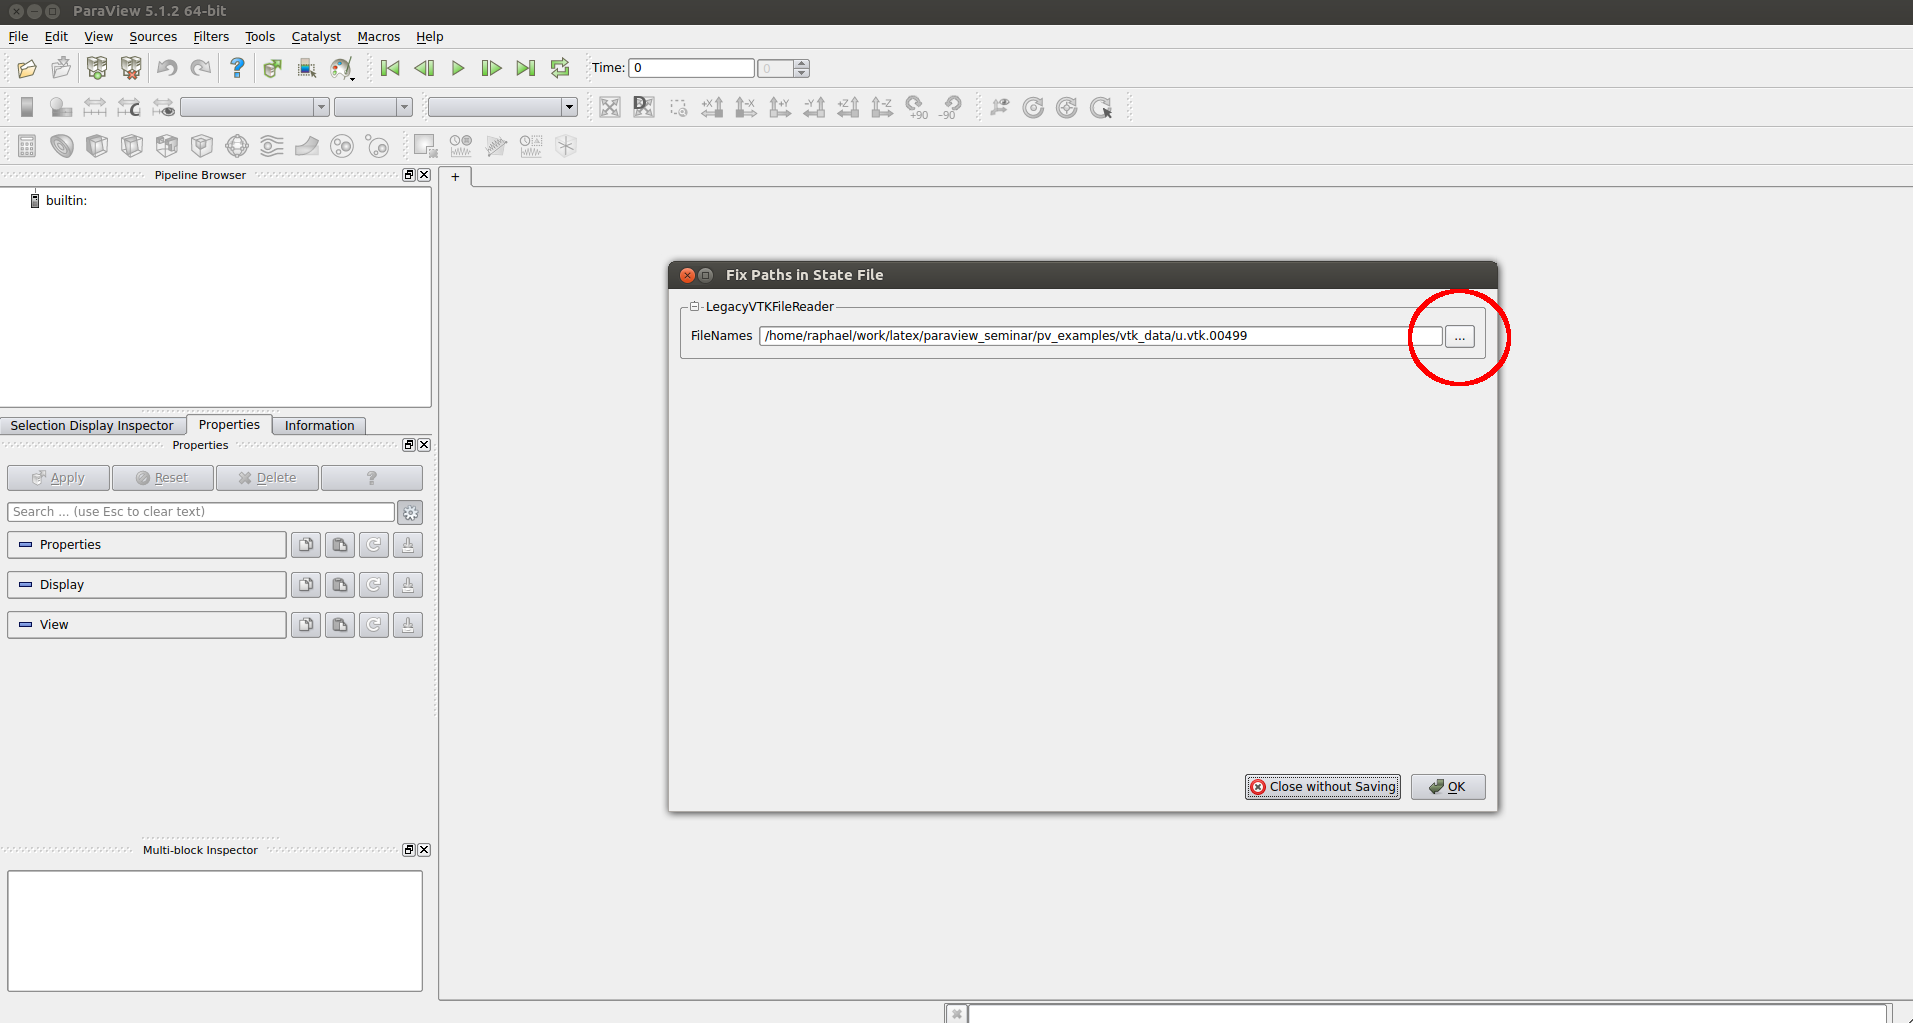
\includegraphics[width=\textwidth]{screenshots/load-state-file.png}
\end{frame}

\begin{frame}
  \frametitle{Examples Files}

    \begin{itemize}
      \item ParaView examples are provided as state files 
      \item Download archive of ParaView examples from:
      \item Extract archive to \kommandozeile{/mypath/to/examples/}
      \kommandozeile{> tar xvfz pv\_examples.tar.gz -C /mypath/to/examples/}
      \item Basic filter examples are located in \kommandozeile{/mypath/to/examples/pv\_examples}
      \item Basic filter examples are located in \kommandozeile{/mypath/to/examples/pv\_examples/BasicFilters}
      \item To load a basic filter example, load the state file and set data path to:
        \kommandozeile{/mypath/to/examples/pv\_examples/vtk\_data/u.vtk}
    \end{itemize}
        

\end{frame}

\begin{frame}
  \frametitle{Basic Filter Gallery I}

    \begin{tikzpicture}%[nodes=draw]

      \node[align=center,scale=0.2,transform shape] (C1) at (0,0)
      {\includegraphics{screenshots/warp-by-scalar.png}};

      \node[align=center,scale=0.2,transform shape] (C2) at (0,-6)
      {\includegraphics{screenshots/contours.png}};

      \node[align=center,scale=0.2,transform shape] (C3) at (12,-6.05)
      {\includegraphics{screenshots/contours_few.png}};

      \node[align=center,scale=0.2,transform shape] (C4) at (12,0)
      {\includegraphics{screenshots/glyphs.png}};

    \end{tikzpicture}

\end{frame}

\begin{frame}

  \frametitle{Basic Filter Gallery II}

    \begin{tikzpicture}%[nodes=draw]

      \node[align=center,scale=0.45,transform shape] (C1) at (0,0)
      {\includegraphics{screenshots/surface_lic_final.png}};

      \node[align=center,scale=0.4,transform shape] (C2) at (0,-6)
      {\includegraphics{screenshots/streamlines.png}};


    \end{tikzpicture}

\end{frame}

\begin{frame}
  \frametitle{Stationary and Transient Data Sets}
    \begin{itemize}
      \item Stationary simulation data usually results in a single file
      \item Transient simulations usually result in a file series 
      \item ParaView recognizes many naming patterns:
      \begin{itemize}
        \item name.0000.vtk, name.0001.vtk, name.0002.vtk,...
        \item name.vtk.0000, name.vtk.0001, name.vtk.0002,...				
      \end{itemize}	
      \item Transient data sets can be 'played' with the animation controls
      \item Without actual timestamps, each file gets assigned one time unit 500 files $\mapsto$ 500 time steps					
    \end{itemize}				
		\begin{center}
      \includegraphics[width=0.9\textwidth]{screenshots/transient.png}					
		\end{center}
\end{frame}

\begin{frame}
  \frametitle{Tracer Filters}
    \begin{itemize}
      \item Visualization of fluid motion by markers/tracers/indicators
      \item Streamlines for stationary vector fields
      \item Visualize the path that a particle would take 
      \item Particle tracers for transient data
      \item Moves particles along a series of vector fields
      \item Final visualization often results in an animation outputted in a movie format (.avi, .mp4, .wmv, ...)
      \item Surface Line Integral Convolution (\keyword{Surface LIC} Plugin) can sometimes be used as an alternative
    \end{itemize}
\end{frame}

\begin{frame}

  \frametitle{Configuration of Tracer Filters}

    \begin{itemize}
      \item Tracer type filters need an \keyword{input data set} and a \keyword{seed source}
      \item The input data set is the the flow field  
      \item The seed source is a user-defined starting location for the particles inside the flow field  
    \end{itemize}
		\begin{center}
    \includegraphics[width=0.5\textwidth]{screenshots/tracer-source.png}			
		\end{center}
\end{frame}

\begin{frame}

  \frametitle{Advanced Filters: Particle Tracer}

    \begin{itemize}
      \item Used to visualize transient flow data by particles 
      \item A particle path is produced by moving a particle along successive vector fields 
      \item Particle movement can then be animated by the \keyword{Animation Control} 
      \item Particle tracer example location: \kommandozeile{/mypath/to/examples/pv\_examples/AdvancedFilters/particle\_tracer}
    \end{itemize}
    \includegraphics[width=\textwidth]{screenshots/particle-tracer.png}

\end{frame}

\begin{frame}

  \frametitle{List of Useful Filters}

    \begin{itemize}
      \item \keyword{Extract Selection}: Extract a subset from a data set (tracer source, plotting, etc)
      \item \keyword{Extract Surface}: Generates a polygonal surface mesh (exporting, rendering, remeshing) 
      \item \keyword{Clean to Grid}: Removes multiply defined simplices and converts to unstructured mesh
      \item \keyword{Integrate Variables}: Performs numerical integration of the fields defined in the data set on the mesh 
      \item \keyword{Iso-Volume or Iso-Surface}: Constructs a volume or a surface from a function defined on the mesh 
      \item \keyword{Plot Over Line}: Generates a plot of data fields along a line (inflow profiles, etc.) 
      \item \keyword{Calculator}: Use a set of mathematical operations to compute a new data field from existing ones (often used together with integrate variables filter)
    \end{itemize}

\end{frame}

\begin{frame}

  \frametitle{Plotting with ParaView}

  \begin{itemize}

      \item PV plotting example: \kommandozeile{/mypath/to/examples/pv\_examples/Plotting/plotting.pvsm}

      \item Common ParaView plotting filters:
      \begin{itemize}

        \item \keyword{Plot Data} 

        \item \keyword{Plot Over Line} 

        \item \keyword{Plot Selection Over Time} 

      \end{itemize}

    \item Data can be exported to .csv to use in your favorite plot generator \keyword{File->Save Data}

    \item ParaView will by default export ALL data fields to the .csv file (even those that you do not want or need for the plot) 

    \item \keyword{Solution 1:} use <awk> to select the data columns you want: \kommandozeile{awk -F \textquotesingle,\textquotesingle $\;$  \textquotesingle\{print \$1 " " \$4\}\textquotesingle} (extract first and fourth column)

    \item \keyword{Solution 2:} Remove unneccessary fields before export: \kommandozeile{/mypath/to/examples/pv\_examples/Plotting/plotting2.pvsm}

  \end{itemize}

\end{frame}

\begin{frame}
  \frametitle{Selecting and Inspecting Data}
    \begin{itemize}
      \item Inspect nodes or elements of special interest in your data set
      \item Locate/Pinpoint a potential or actual cause of problems in your simulation data
      \item Parallel projection mode can be very helpful during manual selection (3D data sets)
      \item Select points elements/points on surface or through frustrum volume
      \item Polygonal selection tool for non-box shaped selections
      \item +/- icon can add/substract from selection
      \item Press 'v' key opens 'Find Data' window to inspect numerical values of selection
    \end{itemize}
		\begin{center}
      \includegraphics[width=0.9\textwidth]{screenshots/selection-icons.png}					
		\end{center}
\end{frame}

\begin{frame}
  \frametitle{Spreadsheet View}
    \begin{itemize}
      \item Shows numerical values of cells/nodes of the data set
      \item Selected elements are highlighted 
    \end{itemize}
		\begin{center}
      \includegraphics[width=0.8\textwidth]{screenshots/spreadsheet.png}					
		\end{center}
\end{frame}

\begin{frame}
  \frametitle{Find Data}
    \begin{itemize}
      \item Shows numerical values of selected elements
      \item \keyword{Freeze Selection} selects elements by ID instead of location in frustrum
    \end{itemize}
		\begin{center}
      \includegraphics[width=0.8\textwidth]{screenshots/find-data.png}					
		\end{center}
\end{frame}

\begin{frame}
  \frametitle{Screenshots With ParaView}
    \begin{itemize}
      \item Screenshots can be made from \keyword{File->Save Screenshots} 
      \item Screenshots size can be set in dialog window
      \item The content of the screenshot is the entire render view
    \end{itemize}
		\begin{center}
      \includegraphics[width=0.6\textwidth]{screenshots/screen-dialog.png}
		\end{center}
\end{frame}

\begin{frame}
  \frametitle{Advanced Screenshot techniques}
    \begin{itemize}
      \item Use split windows to make side-by-side comparisons
      \item Use the text source to add labels to certain elements
      \item Set precise screenshot dimensions with the lock screen function
      \item Background colors can be quickly adjusted by changing the color palette
      \item Font and color of labels and color map widgets can be customized
      \item Visualize edges with tube filter to increase visibility
    \end{itemize}
\end{frame}

\begin{frame}
  \frametitle{Animations/Movies With ParaView}
    \begin{itemize}
      \item Animations can be rendered in ParaView by \keyword{File->Save Animation}
      \item Can be saved as a .png file series or movie format 
      \item Image series can later be compiled into a movie with other programs 
      \item Animation can be configured by \keyword{View->Animation View}
      \item Frames per second, video length, start and end time can be set
    \end{itemize}
\end{frame}

\begin{frame}

  \frametitle{Input Data Formats}

    \begin{itemize}

      \item VTK data formats support polygonal data sets and structured or unstructured meshes 

      \item \keyword{VTK Legacy format .vtk} is a simple format useable for unstructured meshes (not suited for distributed data)  

      \item \keyword{VTK unstructured .vtu} is an xml based format for unstructured meshes   
    \begin{itemize}

      \item Can have the mesh data part encoded in a binary format   

      \item A \keyword{.pvtu} file can be used to reference the partial solutions of a distributed computation   

      \item A \keyword{.pvd} file can be used to add time information   

    \end{itemize}

    \item For further information on VTK file formats see:
      \url{http://www.vtk.org/VTK/img/file-formats.pdf}

  \end{itemize}

\end{frame}

\begin{frame}
  \frametitle{Simple VTK Legacy Cube Data}
		\begin{center}
      \includegraphics[width=0.8\textwidth]{screenshots/cube-vtk.png}					
		\end{center}
\end{frame}

\begin{frame}

  \frametitle{Scripted Postprocessing in ParaView}

  \begin{itemize}

    \item Python interface to access ParaView functionality by scripts

    \item Can be done interactively via a python shell: \keyword{Tools->Python Shell} 

    \item In a 'batch' style by passing a script to the executables \keyword{pvpython} or \keyword{pvbatch} 

    \item Documentation of the ParaView Python interface is under construction at:
      \url{https://www.paraview.org/ParaView3/Doc/Nightly/www/py-doc/}

    \item A trace mechanism is available to generate a PvPython script from a sequence of actions

    \item Beginners should use the trace mechanism (\keyword{Tools->Start Trace}) with the settings \keywords{Show Incremental Trace} and \keywords{only user-modified properties} 

    \item Upon \keyword{Tools->Stop Trace} a file is generated showing the PvPython script equivalent of the user's GUI actions
  \end{itemize}

\end{frame}

\begin{frame}
  \frametitle{Programmable Filters}
\end{frame}

\begin{frame}

  \frametitle{PvPython Simple Example}

  \begin{itemize}
      \item PvPython simple example location: \kommandozeile{/mypath/to/examples/pv\_examples/PvPython/paraview\_python}

      \item Navigate to the folder and execute the PvPython script by: \kommandozeile{pvbatch ./python\_test.py \$(pwd)} or for versions higher than 5.1
        \kommandozeile{pvbatch {-}{-}use-offscreen-rendering ./python\_test.py \$(pwd)}

      \item The script will write an image \keyword{res.png} to the directory where you executed it 
      \item \keyword{Exercise:} Try to recreate the python script using the trace mechanism, compare the output images if they are the same.

      \item \keyword{Hint:} Prefer \keyword{pvbatch} over \keyword{pvpython} as pvpython tries to open an X windows which may fail on some computers    
  \end{itemize}

\end{frame}

\begin{frame}

  \frametitle{When to use PvPython}

  \begin{itemize}

    \item Repeated application of filters to a lot of different data sets (parameterize script w.r.t. data set) 

    \item Repeated application of operations that cannot be parametrized by ParaView GUI

    \item Perform an operation that cannot easily be done by ParaView filters 

    \item Quickly and repeatedly generate an ouput of a running simulation 

    \item Generate outputs on remote clusters 

    \item \keyword{ParaView Programmable Filter} or \keyword{Python Calculator} may serve as an alternative 

  \end{itemize}

\end{frame}



\begin{frame}
  \frametitle{Client-Server Mode}

    \begin{itemize}
      \item In default mode ParaView is both the client and the server
      \item When client/server are different rendering and data processing can
        be handled by different computers 
      \item Simple X forwarding works adequately only if the network speed is fast
      \item Client-Server is preferable to access data on remote (non-local) clusters 
      \item Client-Server steps: \keyword{port forwarding}, \keyword{starting the remote server}, \keyword{connecting the client to the server}  
    \end{itemize}

    \begin{block}{Port Forwarding}
        \begin{itemize}
          \item Establish an ssh tunnel to forward the local port to the remote server: \\  
          \kommandozeile{> ssh lidong1.itmc.tu-dortmund.de \textbackslash}
          \kommandozeile{-L 11111:lidong1.itmc.tu-dortmund.de:11111}
        \end{itemize}
    \end{block}

\end{frame}

\begin{frame}
  %\frametitle{Client-Server Mode II}

    \begin{block}{Start the remote Server}
        \begin{itemize}
          \item Start a ParaView data server on the remote machine  
            \kommandozeile{> pvserver {-}{-}server-port=11111}
        \end{itemize}
    \end{block}

    \begin{block}{Connect to the remote Server}
        \begin{itemize}
          \item Start a ParaView client locally  
          \item Press the <Connect> button on the toolbar  
          \item Manually configure the Server dialog:
          \begin{itemize}
            \item Name: myname   
            \item Server Type: Client/Server  
            \item Host: localhost 
            \item Port: 11111 
          \end{itemize}
        \end{itemize}
    \end{block}
  Pitfalls:
    \begin{itemize}
      \item You \textbf{have to} make use the same ParaView version of the client and the server
      \item Check that the port is not occupied, otherwise use a different port: 
      \kommandozeile{> lsof -i:11111}
    \end{itemize}

\end{frame}

\begin{frame}

  \frametitle{Additional ParaView Resources}

  \begin{itemize}
      \item ParaView documentation:\\
        \url{https://www.paraview.org/documentation/}
      \item ParaView Wiki:\\
        \url{https://www.paraview.org/Wiki/ParaView}
      \item ParaView Tutorial:\\
        \url{https://www.paraview.org/Wiki/The\_ParaView\_Tutorial}
      \item ParaView Mailing List:\\
        \url{https://public.kitware.com/mailman/listinfo/paraview}
      \item ParaView Catalyst:\\
        \url{https://www.paraview.org/Wiki/ParaView/Catalyst/Overview}
      \item ParaView Web JavaScript:\\
        \url{www.paraview.org/Wiki/ParaViewWeb\_JavaScript\_Introduction}
  \end{itemize}

\end{frame}


%
\begin{frame}
	\frametitle{About Matplotlib}

    \begin{itemize}
    \item Python-based, open-source plotting library
    \item Available for all Python installations for different operating systems
    \item Uses data structures from other Python libraries like NumPy
    \item Integrates well with Python scientific libraries (NumPy, SciPy,...)
    \item Together with these libraries provides Matlab-like functionality 
    \item Access to Python file processing functions for convenient, cross-platform data handling 
    \item Can by used interactively in environments like Jupyter or in batch mode
    \item Plots can be saved in various file formats including PNG bitmap and PDF vector graphics
    \end{itemize}

\end{frame}

\begin{frame}
	\frametitle{Installation}
    \begin{itemize}
      \item For Windows and macOS:		
      \item Anaconda Python: https://www.anaconda.com/products/individual
			\item If not included: \kommandozeile{conda install -c conda-forge matplotlib}      
      \item Linux variants:
      \item Use package manager to install python
			\item Use pip to install matplotlib: \kommandozeile{pip install -U matplotlib}
			\item Use Jupyter online to try it online: https://jupyter.org/try
			\item Anaconda install Jupyter Windows/macOS: \kommandozeile{conda install ipython jupyter}
			\item Pip install Jupyter: \kommandozeile{pip install --upgrade ipython jupyter}
    \end{itemize}
\end{frame}

\begin{frame}
    \begin{center}
      \includegraphics[width=0.9\textwidth]{screenshots/jupyter-1.png}
    \end{center}		
\end{frame}

\begin{frame}
	\frametitle{Start a Juypter Notebook}
    \begin{itemize}
      \item Command line, Terminal or CMD: \kommandozeile{jupyter notebook}
      \item Runs in browser window
			\item In Visual Studio Code with Python Extension: 
			\item \keyword{STRG + SHIFT + P->Jupyter: Create New Blank Jupyter Notebook} 			
    \end{itemize}
    \begin{center}
      \includegraphics[width=1.0\textwidth]{screenshots/vsc-2.png}
    \end{center}				
\end{frame}

\begin{frame}
    \begin{center}
      \includegraphics[width=0.9\textwidth]{screenshots/vsc-1.png}
    \end{center}				
\end{frame}

\begin{frame}[fragile]
	\frametitle{Matplotlib from the Command Line}
    \begin{itemize}
      \item Create a file \keyword{my-first-plot.py}
    \end{itemize}
    \begin{block}{File: my-first-plot.py}
    \begin{lstlisting}[language=Python]
    import matplotlib.pyplot as plt
    plt.plot([1,2,3,4], [1, 4, 9, 16], color="red")
    plt.show()
    \end{lstlisting}      
		\end{block}		
    \begin{itemize}
      \item Run the python script \keyword{python ./my-first-plot.py}
    \end{itemize}			
    \begin{center}
      \includegraphics[width=0.25\textwidth]{screenshots/plt-2.png}
    \end{center}						
\end{frame}

\begin{frame}[fragile]
   \vspace{-1cm}
    \begin{center}
      \includegraphics[width=0.7\textwidth]{screenshots/plt-1.png}
    \end{center}						
\end{frame}

\begin{frame}[fragile]
	\frametitle{Components of a Matplotlib Plot}
    \begin{itemize}
      \item \keyword{Figure (object)}: The top-level component, the whole window/container of the plot
      \item \keyword{Axes}: The area containing the plot data, labels, axis ticks, etc. 
      \item The term \keyword{Subplot} in Matplotlib is in most cases the same as \keyword{Axes} 
      \item \keyword{XAxis} and \keyword{YAxis}: Are the corresponding parts of the \keyword{Axes} object
      \item Knowledge of these components makes it easier to add/change properties 
    \end{itemize}
\end{frame}

\begin{frame}[fragile]
   \vspace{-1cm}
    \begin{center}
      \includegraphics[width=0.7\textwidth]{screenshots/plt-3.png}
    \end{center}						
\end{frame}

\begin{frame}[fragile]
	\frametitle{Reading Data from a File}
    \begin{itemize}
      \item Create a file \keyword{my-second-plot.py}
    \end{itemize}
    \begin{block}{File: my-second-plot.py}
    \begin{lstlisting}[language=Python]
    import matplotlib.pyplot as plt
		import numpy as np
    data = np.loadtxt("data.txt")
    plt.plot(data[:,0], data[:,1], color="red")
		plt.show()
    \end{lstlisting}      
		\end{block}		
    \begin{itemize}
      \item Run the python script \keyword{python ./my-second-plot.py}
    \end{itemize}			
\end{frame}

\begin{frame}[fragile]
	\frametitle{Setting Axes Properties Explicitly}
    \begin{block}{File: plot-explicit.py}
    \begin{lstlisting}[language=Python]
import matplotlib.pyplot as plt
fig = plt.figure()
ax = fig.add_subplot(111)
ax.plot([1, 2, 3, 4], [10, 20, 25, 30], color='lightblue',
       linewidth=3)
ax.scatter([0.3, 3.8, 1.2, 2.5], [11, 25, 9, 26], 
          color='darkgreen', marker='^')
ax.set_xlim(0.5, 4.5)
plt.show()
    \end{lstlisting}      
		\end{block}		
\end{frame}

\begin{frame}[fragile]
	\frametitle{Setting Axes Properties Implicitly}
    \begin{block}{File: plot-implicit.py}
    \begin{lstlisting}[language=Python]
import matplotlib.pyplot as plt		
plt.plot([1, 2, 3, 4], [10, 20, 25, 30], color='lightblue',
        linewidth=3)
plt.scatter([0.3, 3.8, 1.2, 2.5], [11, 25, 9, 26], 
           color='darkgreen', marker='^')
plt.xlim(0.5, 4.5)
plt.show()
    \end{lstlisting}      
		\end{block}
    \begin{itemize}
      \item \keyword{Axes} functions/methods are called "behind the scenes"
      \item If multiple axes/subplots are present then use Axes object directly			
    \end{itemize}		
\end{frame}

\begin{frame}[fragile]
   \vspace{-1cm}
    \begin{center}
      \includegraphics[width=0.7\textwidth]{screenshots/fig-ex-1.png}
    \end{center}						
\end{frame}

\begin{frame}[fragile]
	\frametitle{Using the API Documentation}
    \begin{itemize}
      \item https://matplotlib.org/contents.html
    \end{itemize}			
   \vspace{2cm}			
    \begin{center}
      \includegraphics[width=0.8\textwidth]{screenshots/manual-api.png}
    \end{center}						
\end{frame}

\begin{frame}[fragile]
	\frametitle{Plot Customization}
    \begin{block}{File: plot-custom-1.py}
    \begin{lstlisting}[language=Python]
X = np.linspace(-np.pi, np.pi, 256, endpoint=True)
Cos, Sin = np.cos(X), np.sin(X)
plt.plot(X, Cos, color="blue", linewidth=2.5, linestyle="-", label="Kosinus")
plt.plot(X, Sin, color="red",  linewidth=2.5, linestyle="--", label="Sinus")
# Gitter 
plt.grid()
# Titel
plt.title("Sinus und Kosinus",loc="center")
# Legende
plt.legend(loc="best", frameon=False)
    \end{lstlisting}      
		\end{block}
\end{frame}

\begin{frame}[fragile]
   \vspace{-1cm}
    \begin{center}
      \includegraphics[width=0.9\textwidth]{screenshots/plt-4.pdf}
    \end{center}						
\end{frame}

\begin{frame}[fragile]
	\frametitle{Plot Customization II}
    \begin{block}{File:  plot-custom-1.py continued}
    \begin{lstlisting}[language=Python]
# Legende
plt.legend(loc="best", frameon=True)
plt.xticks([-np.pi, -np.pi/2, 0, np.pi/2, np.pi],
       [r'$-\pi$', r'$-\pi/2$', r'$0$', r'$+\pi/2$', r'$+\pi$'])
plt.yticks([-1, 0, +1],
       [r'$-1$', r'$0$', r'$+1$'])
    \end{lstlisting}      
		\end{block}
    \begin{itemize}
      \item r'text' is a raw string
      \item Inside a raw string \$ can be used to enter latex equations
    \end{itemize}					
\end{frame}

\begin{frame}[fragile]
   \vspace{-1cm}
    \begin{center}
      \includegraphics[width=0.85\textwidth]{screenshots/plt-5.png}
    \end{center}						
\end{frame}

\begin{frame}[fragile]
	\frametitle{Plot Customization III}
    \begin{itemize}
      \item Highlight data points using the \keyword{annotate} function
      \item Configure the \keyword{spines} of the subplot
      \item \keyword{Spines} are the 4 lines bordering the plot area 
      \item Stored in python dictionary with keys: 'top', 'left', 'bottom', 'right'
      \item Text labels usually have a fontsize	property that can be adjusted		
    \end{itemize}					
\end{frame}

\begin{frame}[fragile]
   \vspace{-1cm}
    \begin{center}
      \includegraphics[width=0.85\textwidth]{screenshots/plt-6.png}
    \end{center}						
\end{frame}

\begin{frame}[fragile]
	\frametitle{Subplots and Plot Types}
    \begin{itemize}
      \item Subplots can be grouped in a grid of plots
    \begin{block}{Create subplot with two rows and columns}
    \begin{lstlisting}[language=Python]
			fig, axes = plt.subplots(nrows=2, ncols=2)		
			# Set title for a single subplot
			axes[1,0].set_title('Title for 2nd row 1st column')
    \end{lstlisting}      
		\end{block}
      \item Large variety of plot types as in Matlab
      \item Bar plot, pie plot, contour plot, histograms, stream plots, 3D plots, $\ldots$ 
			\item \url{https://matplotlib.org/tutorials/introductory/sample_plots.html}
    \end{itemize}					
\end{frame}

\begin{frame}[fragile]
   \vspace{-1cm}
    \begin{center}
      \includegraphics[width=0.7\textwidth]{screenshots/plt-8.png}
    \end{center}						
\end{frame}

\begin{frame}[fragile]
	\frametitle{Saving Plots to a File from a Script}
    \begin{itemize}
      \item Subplots can be grouped in a grid of plots			
    \begin{block}{plot-savefig.py}
    \begin{lstlisting}[language=Python]			
			fig, ax = plt.subplots()			
			ax.plot(t, s)
			ax.set(xlabel='time (s)', ylabel='voltage (mV)',
						 title='A Simple Plot')
			ax.grid()
			fig.savefig("test.pdf")			
    \end{lstlisting}      
		\end{block}						
    \end{itemize}					
\end{frame}

\begin{frame}[fragile]
	\frametitle{Using Matplotlib on a Cluster without Graphical Interface}
    \begin{itemize}
      \item Design your desired postprocessing plot in i.e. Jupyter notebook
      \item Save your python code to a script, eventually add file handling/manipulation code			
      \item Add code to save your plot to a file				
      \item Transfer the script to the compute cluster						
      \item Execute script on the cluster, transfer the resulting file to local computer									
    \end{itemize}					
\end{frame}
%\begin{frame}
%	\begin{block}{\huge Aufgabe 1 (Hello World)}
%		Erstellen Sie folgendes "Hello-World" Beispiel.
\begin{verbatim}
\documentclass{article}
\begin{document}
    Hello World!
\end{document}
\end{verbatim}
%	\end{block}
%\end{frame}
%\begin{frame}
	\frametitle{Spezielle Zeichen}
	\begin{itemize}
		\item bei Verwendung des ASCII-Zeichensatzes: Buchstaben ohne Umlaute, Zahlen und einige Sonderzeichen
		\item manche Zeichen sind \LaTeX-Steuerzeichen und daher reserviert (\$, \_, \{, \},\textbackslash )
        \item solche Sonderzeichen können durch \textbackslash{} maskiert werden: \\[0.5cm]
		\begin{center}
			\begin{tabular}{|cc|cc|} \hline
				\$ & \textbackslash\$ & \% & \textbackslash\% \\
				\{ & \textbackslash\{ & \} & \textbackslash\} \\
				\# & \textbackslash\# & \_ & \textbackslash\_ \\
				\& & \textbackslash\& & & \\ \hline
			\end{tabular}
		\end{center}
	\end{itemize}
\end{frame}

\begin{frame}[fragile]
	\frametitle{Deutsche Texte - Sprachpakete}
    Ohne weitere Angaben nimmt \LaTeX{} an, dass der eingegebene Text in englischer Sprache ist. Daher muss ggf. ein zusätzliches Sprachpaket eingebunden werden:
	\begin{center}
		\begin{block}{Beispiel-Header: deutsches Sprachpaket}
			\begin{lstlisting}
\documentclass[a4paper]{article}      % DIN-A4 Papierformat
\usepackage[ngerman]{babel}           % deutsche Benennung
\usepackage[utf8]{inputenc}
\begin{document}
  ...
\end{document}
			\end{lstlisting}
		\end{block}
	\end{center} \vspace{-1cm}
	\begin{itemize}
		\item \keyword{babel} sorgt für Unterstützung anderer Sprachen (Formate, Umlaute, Benennungen, Silbentrennung)
		\item \keyword{inputenc} unterstützt die direkte Eingabe von Zeichen über die Tastatur
	\end{itemize}
\end{frame}


\begin{frame}[fragile]
	\frametitle{Deutsche Texte -- Umlaute und Anführungszeichen}
	
	Eingabe deutscher Texte:
	\begin{itemize}
		\item Umlaute: \befehl{"a}, \befehl{"o}, \befehl{"u}, \befehl{ss} für ä, ö, ü, ß
		\item Anführungszeichen: \befehl{glq}, \befehl{grq} bzw. \befehl{glqq}, \befehl{grqq} für \glq einfache\grq~ bzw. \glqq doppelte\grqq~ Anführungszeichen
	\end{itemize}
	\vfill
	
	\latexBeispielDirekt{Beispiel: deutsche Umlaute}{examples/Deutsche_Umlaute/Deutsche_Umlaute}
	\vfill
\end{frame}

\begin{frame}[fragile]
	\frametitle{Deutsche Texte - Silbentrennung}
	\begin{itemize}
		\item erfolgt automatisch
		\item mögliche Trennstellen können  durch \befehl{-} auch angegeben werden, z. B.\\
		\lstinline$Donau\-dampf\-schiff\-fahrts\-gesell\-schaft$\\
		oder für das gesamte Dokument in der Präambel:
		\lstinline$\hypenation{Donau\-dampf\-schiff\-fahrts\-gesell\-schaft}$
	\end{itemize}

\end{frame}

%
%\begin{frame}[fragile]
	\frametitle{Textformatierung -- Schriftstil}
	
	\begin{center}
		\begin{tabular}{l|ll|l}
			Familie & \multicolumn{2}{c|}{Befehle} & Beispiel \\ \hline
			normal (mit Serifen) & \befehl{rmfamily} & \befehl{textr} & \textrm{normal} \\
			serifenfrei & \befehl{sffamily} & \befehl{textsf} & \textsf{serifenfrei} \\
			Schreibmaschine & \befehl{ttfamily} & \befehl{texttt} & \texttt{Schreibmaschine} \\
		\multicolumn{4}{c}{~} \\
			Varianten & \multicolumn{2}{c|}{Befehle} & Beispiel \\ \hline
			aufrecht & \befehl{upshape} & \befehl{textup} & \textup{aufrecht} \\
			italic & \befehl{itshape} & \befehl{textit} & \textit{italic}\\
			Kapitälchen & \befehl{scshape} & \befehl{textsc} & \textsc{Kapitälchen}\\
			fett & \befehl{bfseries} & \befehl{textbf} & \textbf{fett}\\
			unterstrichen & ~ & \befehl{underline} & \underline{unterstrichen}
		\end{tabular}
	\end{center}
\end{frame}

\begin{frame}[fragile]
	\frametitle{Textformatierung -- Schriftgröße}
	\begin{center}
		\begin{tabular}{ll}
		\befehl{tiny} & \tiny{winzig} \\
		\befehl{small} & \small{klein} \\
		\befehl{footnotesize} & {\fontsize{14}{14}\selectfont{}Fußnotengröße}\\
		\befehl{normalsize} & normale Größe\\
		\befehl{large} & {\fontsize{25}{25}\selectfont{}groß} \\
		\befehl{Large} & {\fontsize{30}{30}\selectfont{}größer} \\
		\befehl{huge} & {\fontsize{40}{40}\selectfont{}riesig} \\
		\befehl{Huge} & {\fontsize{50}{50}\selectfont{}Riesig}
		\end{tabular}
	\end{center}
	\vfill
	\begin{itemize}
		\item für einige Wörter: \lstinline${\huge riesig}$
		\item für ganze Absätze: \lstinline$\begin{tiny} ... \end{tiny}$
		\item alternativ: punktgenau durch \lstinline${\fontsize{40}{48}\selectfont{}Test}$\\
		das erste Argument gibt die Schriftgröße an, das zweite den Grundlinienabstand
	\end{itemize}
\end{frame}



%\begin{frame}[fragile]
	\frametitle{Textformatierung -- minipages}
	\begin{itemize}
		\item die \keyword{minipage}-Umgebung wird genutzt, wenn in Boxen komplexere Inhalte  dargestellt werden sollen
		\item es muss die Breite angegeben werden
	\end{itemize}
	\latexBeispielDirekt{Beispiel: minipages}{examples/minipages/minipages.tex}
\end{frame}

\begin{frame}[fragile]
	\frametitle{Textformatierung -- Absatzausrichtung} \vspace{-0.7cm}
	\latexBeispielDirekt{Beispiel: Absatzausrichtung}{examples/absatzausrichtung/absatzausrichtung.tex}
	\vfill
\begin{itemize}
	\item Standard: Blocksatz
	\item alternativ kann man auch die Befehle \befehl{raggedleft}, \befehl{raggedright} und \befehl{centering} verwenden (statt den obigen Umgebungen)
\end{itemize}
\end{frame}

\begin{frame}[fragile]
	\frametitle{Textformatierung - Zitate und Gedichte}
	\latexBeispielDirektKlein{Beispiel: Zitate und Gedichte}{examples/Zitate_und_Gedichte/Zitate_und_Gedichte.tex}
\end{frame}

\begin{frame}[fragile]
	\frametitle{Text ohne Formatierung}
	\begin{itemize}
		\item um Programmcode oder Beispiele ohne Formatierung auszugeben, gibt es die \keyword{verbatim}-Umgebung
		\item innerhalb eines Textes kann man den Befehl \befehl{verb} nutzen; das erste Zeichen nach dem Befehl wird dann als Endmarker interpretiert
	\end{itemize}\vfill
	\latexBeispielDirekt{Beispiel: \keyword{verbatim}-Umgebung}{examples/verbatim/verbatim.tex}
\end{frame}

\begin{frame}[fragile]
	\frametitle{Randnotizen und Fußnoten}
	\latexBeispielDatei{Beispiel: Randnotiz und Fußnote}{examples/Randnotiz_und_Fussnote/Randnotiz_und_Fussnote}
\end{frame}
%%\begin{frame}[fragile]
	\frametitle{Dokumentenklasse}
	
	\begin{block}{Allgemeine Form}
		\lstinline$\documentclass[option1,option2]{klasse}$
	\end{block}
	\vfill
	einige verfügbare Klassen:
	\begin{itemize}
		\item \emphkeyword{article}, \emphkeyword{scrartcl} für Artikel, Ausarbeitungen oder Berichte
		\item \emphkeyword{report}, \emphkeyword{scrreprt} für Ausarbeitungen, Diplomarbeiten, Skripten oder Dissertationen
		\item \emphkeyword{book}, \emphkeyword{scrbook} für Bücher
		\item \emphkeyword{letter}, \emphkeyword{scrlttr2} für Briefe
	\end{itemize}
	\vfill
\end{frame}


\begin{frame}[fragile]
	\frametitle{Dokumentenklasse -- häufig benutzte Optionen}
	
	\begin{tabular}{rl}
		\emphkeyword{draft} & Entwurfsmodus (markiert überstehenden Text, zeigt Grafiken als Box) \\
		\emphkeyword{11pt} & Schriftgr\"o\ss{}e 11 Punkte \\
		\emphkeyword{12pt} & Schriftgr\"o\ss{}e 12 Punkte\\
		\emphkeyword{a4paper} & Gr\"o\ss{}en anpassen f\"ur Din A4\\
		\emphkeyword{titlepage} & Titelseite erzwingen f\"ur \keyword{\texttt{article}}\\
		\emphkeyword{twocolumn} & zweispaltiges Dokument\\
		\emphkeyword{twoside} & Vorder- und R\"uckseite der Seiten wird bedruckt\\
		\emphkeyword{fleqn} & Formeln linksb\"undig setzen\\
		\emphkeyword{leqno} & Nummerierung von Formeln links statt rechts
	\end{tabular}
\end{frame}


\begin{frame}
	\frametitle{Titelseite aus Metadaten}
	
	\only<1>{
	\latexBeispielDateiCodeAnmerkungen{automatisch generierte Titelseite}{examples/Titelseite/Titelseite}{
	\begin{tabular}{rp{6cm}}
		\keyword{\~} & unzerbrechliches Leer\-zeichen\\
		\befehl{title} & Titel des Dokuments \\
		\befehl{author} & Autoren (Schlüsselwort \befehl{and} bei Angabe mehrerer Autoren) \\
		\befehl{date} & Veröffentlichungsdatum\\
		\befehl{maketitle} & generiert die Titelseite aus den Metadaten
	\end{tabular}
	}}
	\only<2>{\latexBeispielDatei{automatisch generierte Titelseite}{examples/Titelseite/Titelseite}}
\end{frame}

\begin{frame}
	\frametitle{Eigene Titelseiten}
	\begin{itemize}
		\item um die Titelseite selbst zu gestalten, kann man die \emphkeyword{titlepage}-Umgebung nutzen
	\end{itemize} \vfill
		\latexBeispielDirektFake{Beispiel: eigene Titelseite}{examples/Eigene_Titelseite/Eigene_Titelseite}{\textbf{\Huge Nicht wichtig}\\geschrieben von mir\ldots} \vfill
	\begin{itemize}
		\item die Titelseite taucht an der Stelle im Text auf, an der sie definiert wird
		\item bei einigen Dokumentenklassen (z. B. \emphword{book}) nimmt die Titelseite auch eine ganze Seite ein
	\end{itemize}
\end{frame}

\begin{frame}[fragile]
	\frametitle{Abstract (Zusammenfassung)}
	\begin{itemize}
		\item durch die \emphkeyword{abstract}-Umgebung kann man eine Zusammenfassung des Inhalts angeben
	\end{itemize} \vfill
	\latexBeispielDirektFake{Beispiel: Abstract (Zusammenfassung)}{examples/abstract/abstract}{
	\begin{center} \textbf{\LARGE Abstract} \end{center} \noindent \ldots Zusammenfassung des Textes \ldots} \vfill
	\begin{itemize}
        \item der angezeigte Name \glqq Abstract\grqq{} kann individualisiert werden:\\
		\lstinline$\renewcommand{\abstractname}{MeinName}$
	\end{itemize}
\end{frame}

\begin{frame}
	\frametitle{Strukturierung des Dokuments}
	
	\begin{itemize}
		\item Gliederung in Kaptiel und Unterkapitel
		\begin{itemize}
			\item \befehl{part\{\}} (nicht in allen Dokumentklassen)
			\item \befehl{chapter\{\}} (nicht in allen Dokumentklassen)
			\item \befehl{section\{\}}
			\item \befehl{subsection\{\}}
			\item \befehl{subsubsection\{\}}
			\item \befehl{paragraph\{\}}
			\item \befehl{subparagraph\{\}}
		\end{itemize}
		\item in den geschweiften Klammern \{\} kann der Name des jeweiligen (Unter-)Kapitels angegeben werden
		\item mit dem Befehl \befehl{appendix} kann markiert werden, dass die nachfolgenden (Unter-)Kapitel zum Anhang gehören
	\end{itemize}
\end{frame}

\begin{frame}[fragile]
	\frametitle{Mehrere Quelldateien}
	\begin{itemize}
		\item um Quelltext aus einer anderen Datei einzufügen, wird der \befehl{input}-Befehl genutzt\\
		\lstinline$\input{datei}$
		\item um ganze Kapitel einzubinden, verwendet man stattdessen den Befehl\\
		\lstinline$\include{kapitel}$
		\item zur Gliederung des \LaTeX-Quellcodes schreibt man Kapitel in jeweils eigene Dateien\\
		\lstinline$\include{kapitel1}$\\
		\lstinline$\include{kapitel2}$\\
		usw.
	\end{itemize}
\end{frame}

%\begin{frame}
%	\vspace{-1cm}
%	\begin{block}{\huge Aufgabe 2 (Ein erstes Dokument)}
%		Erstellen Sie ein einfaches \LaTeX-Dokument. Teilen Sie den Text in Kapitel und Unterkapitel ein. Setzen Sie einige Wörter im Text kursiv, im Fettdruck oder in Schreibmaschinenschrift und in verschiedenen Schriftgrößen. Verwenden Sie zum Beispiel das Paket \keyword{blindtext} zur Erzeugung von Text-Passagen.
%	\end{block}
%	\vfill
%	\begin{block}{\huge Aufgabe 3 (Umlaute)}
%		Geben Sie in einem \LaTeX-Dokument die deutschen Umlaute Ä, Ö, Ü, ä, ö, ü, ß aus, indem Sie:
\begin{itemize}
	\item die Umlaute maskieren,
	\item die Umlaute im Quellcode direkt verwenden und den Zeichensatz entsprechend anpassen.
\end{itemize}
%	\end{block}
%\end{frame}
%\begin{frame}
%	\begin{block}{\huge Aufgabe 4 (Zusammensetzen des Dokuments aus mehreren Dateien)}
%			Erstellen Sie ein Dokument aus den bisherigen Aufgaben, welches aus mehreren Dateien besteht. In der Hauptdatei sollen die Präambel, die Titelseite und das Inhaltsverzeichnis stehen. Jedes Kapitel der obersten Ebene soll in einer eigenen Datei stehen und in die Hauptdatei mittels \befehl{include} eingebunden werden. Hierzu müssen die Dateien der vorherigen Aufgaben in ein neues Verzeichnis kopiert werden und die Befehle \befehl{documentclass} und die \keyword{document}-Umgebung aus den vorherigen Aufgaben entfernt werden, da diese sonst doppelt vorhanden wären.
		 

%	\end{block}
%\end{frame}
%\begin{frame}[fragile]
	\frametitle{Aufzählungen}
	\vspace{-0.5cm}
	drei Grundarten von Aufzählungen: \\
	\begin{tabular}{rl}
		\emphkeyword{itemize} & einfache Aufzählung\\
		\emphkeyword{enumerate} & nummerierte Aufzählung\\
		\emphkeyword{description} & Beschreibung
	\end{tabular}\par \vfill
	
	\begin{columns}[T]
		\begin{column}{0.31\textwidth}
			\begin{block}{\tt\bfseries itemize}
				\begin{itemize}
					\item A \item B \item C
				\end{itemize} 
				\begin{lstlisting}
\begin{itemize}
  \item A
  \item B
  \item C
\end{itemize}
				\end{lstlisting}
			\end{block}
		\end{column}
		\begin{column}{0.31\textwidth}
			\begin{block}{\tt\bfseries enumerate}
				\begin{enumerate}
					\item A \item B \item C
				\end{enumerate} 
				\begin{lstlisting}
\begin{enumerate}
  \item A
  \item B
  \item C
\end{enumerate}
				\end{lstlisting}
			\end{block}
		\end{column}
		\begin{column}{0.31\textwidth}
			\begin{block}{\tt\bfseries description}
				\begin{description}
					\item[A] \ldots \item[B] \ldots \item[C] \ldots
				\end{description} 
				\begin{lstlisting}
\begin{description}
  \item[A] \ldots
  \item[B] \ldots
  \item[C] \ldots
\end{description}
				\end{lstlisting}
			\end{block}
		\end{column}
	\end{columns}
\end{frame}

\begin{frame}[fragile]
	\frametitle{Verschachtelte Aufzählungen}
	\vspace{-0.9cm}
	\latexBeispielDirekt{Beispiel: verschachtelte Aufzählung}{examples/Verschachtelte_Aufzaehlung/Verschachtelte_Aufzaehlung}
\end{frame}
%\begin{frame}
%	\begin{block}{\huge Aufgabe 5 (Listen und Aufzählungen)}
%		Erstellen Sie ein Kochrezept. Verwenden Sie für die Zutatenliste die Aufzählungs-Umgebung \keyword{itemize} und für die Zubereitungshinweise die \keyword{enumerate}-Umgebung.
%	\end{block}
%\end{frame}
%\begin{frame}[fragile]
	\frametitle{Tabellen - ein einfaches Beispiel}
	\vspace{-0.9cm}
	\latexBeispielDirekt{Beispiel: einfache Tabelle}{examples/Tabelle_einfach/Tabelle_einfach}
	\vfill
	Tabellenformatierung:\\[0.2cm]
	\begin{tabular}{rlcrl}
		\emphkeyword{l} & linksbündig ausrichten &~~~~~~ & \emphkeyword{|} & einfacher vertikaler Trennstrich \\
		\emphkeyword{c} & zentriert ausrichten && \emphkeyword{||} & doppelter vertikaler Trennstrich\\
		\emphkeyword{r} & rechtsbündig ausrichten && \emphkeyword{@\{text\}} & benutzerdefiniertes Trennzeichen \\
		\emphkeyword{p\{n\}} & Spalte mit fester Breite \keyword{n}
	\end{tabular}
\end{frame}

\begin{frame}
	\frametitle{Tabellen - mehrspaltige Zellen}
	\vspace{-0.9cm}
	\latexBeispielDirekt{Beispiel: mehrspaltige Zellen}{examples/Tabelle_multicolumn/Tabelle_multicolumn}
	\vfill
	Tabellenformatierung:\\[0.2cm]
	\begin{tabular}{rl}
		\emphkeyword{\textbackslash{}hline} & horizontale Linie über die ganze Breite \\
		\emphkeyword{\textbackslash{}vline} & vertikaler Line innerhalb einer Zeile \\
		\emphkeyword{\textbackslash{}cline\{m-n\}} & horizontale Linie von Spalte \keyword{m} bis Spalte \keyword{n}\\
		\emphkeyword{\textbackslash{}multicolumn\{n\}\{format\}\{Inhalt\}} & Zelle über \keyword{n} Spalten
	\end{tabular}
\end{frame}
%\begin{frame}
%	\begin{block}{\huge Aufgabe 6 (Tabellen)}
%		Erstellen Sie folgende Tabellen:
	\begin{center}
		\shadowbox{
			\begin{minipage}{0.9\textwidth}
				\begin{center}
					\begin{tabular}{r|c|l}
						\textbf{rechts} & \textbf{zentriert} & \textbf{links} \\
						\hline\hline
						Hier & steht & ganz \\
						viel & unwichtiger & Text	
					\end{tabular}					
					~~~		
					\begin{tabular}{|r|*{6}{r}|}
						\hline
						$\cdot$ &  1 &  2 &  3 &  4 & $x$ & $y$  \\ \hline
						1 & 1 & 2 & 3 & 4 & $?$ & $?$ \\
						2 & 2 & 4 & 6 & 8 & $*$ & $*$ \\
						\cline{6-7}
						3 & 3 & 6 & 9 & 12 & \multicolumn{2}{|c|}{?} \\
						\cline{6-7}
						4 & 4 & 8 & 12 & 16 & 4$x$ & \vdots \\
						\hline
					\end{tabular}
				\end{center}
			\end{minipage}
		}
	\end{center}

%	\end{block}
%\end{frame}
%
\begin{frame}[fragile]
	\frametitle{Mathematik -- Formeln im Fließtext}
	\begin{itemize}
        \item Formeln müssen in \LaTeX{} markiert werden, damit sie korrekt interpretiert werden
		\item im Mathematik-Modus werden Leerzeichen ignoriert und Buchstabenketten als einzelne Zeichen betrachtet
	\end{itemize}
	\vfill
	\latexBeispielDirekt{Beispiel: Formeln im Fließtext}{examples/Formeln_im_Fliesstext/Formeln_im_Fliesstext}
\end{frame}

\begin{frame}[fragile]
	\frametitle{Mathematik -- Formeln in eigenem Absatz}
	\begin{itemize}
		\item soll eine Formel abgesetzt dargestellt werden, so benutzt man die \keyword{displaymath}-Umgebung oder die Kurzschreibweise \lstinline$\[...\]$
	\end{itemize}
	\vfill
	\latexBeispielDirekt{Beispiel: Formeln in eigenem Absatz}{examples/Formeln_eigener_Absatz/Formeln_eigener_Absatz}
\end{frame}

\begin{frame}[fragile]
	\frametitle{Mathematik -- nummerierte Gleichungen}
	\begin{itemize}
		\item Gleichungen können mit der \keyword{equation}-Umgebung automatisch fortlaufend nummeriert werden
		\item mittels der \keyword{align}-Umgebung können mehrzeilige Formeln nummeriert und ausgerichtet werden
		\item \befehl{nonumber} unterdrückt in der \keyword{align}-Umgebung die Nummerierung einer Zeile
	\end{itemize}
	\vfill
	\latexBeispielDirektKlein{Beispiel: mehrzeilige Gleichungen}{examples/Formeln_mehrzeilig/Formeln_mehrzeilig}
\end{frame}


%\begin{frame}[fragile]
	\frametitle{Mathematik -- Unterschiede bei der Darstellung}
	\begin{itemize}
		\item Formeln werden innerhalb der \keyword{math}-Umgebung anders dargestellt als in der \keyword{displaymath}-Umgebung
	\end{itemize}
	\begin{center}
		\begin{tabular}{c|c|c}
			\LaTeX-Befehl & \keyword{math} & \keyword{displaymath} \\ \hline
			\lstinline$\lim_{x \ra \infty} \ra 0$
			&
			\begin{math}
				\lim_{x \to \infty} \ra 0
			\end{math}
			&\begin{minipage}{4cm}
				\begin{displaymath}
					\lim_{x \ra \infty} \ra 0
				\end{displaymath}
			\end{minipage}
		\end{tabular}
	\end{center}
	\begin{itemize}
		\item mit dem Befehl \befehl{displaystyle} bzw. \befehl{textstyle} kann das jeweils andere Verhalten erzwungen werden
	\end{itemize}
	\latexBeispielDirekt{Beispiel: \keyword{textstyle} und \keyword{displaystyle}}{examples/Formeln_Darstellung/Formeln_Darstellung}
\end{frame}

\begin{frame}
	\frametitle{Mathematik -- Symbole}
	
	\emphword{Logik}
	\begin{center}
		\begin{tabular}{ll|ll|ll|ll|ll}
			\befehl{exists} & $\exists$ & \befehl{forall} & $\forall$ & \befehl{neg} & $\neq$ & \befehl{in} & $\in$ & \befehl{emptyset} & $\emptyset$ \\
			\befehl{notin} & $\notin$ & \befehl{ni} & $\ni$ & \befehl{land} & $\land$ & \befehl{lor} & $\lor$ & \befehl{varnothing} & $\varnothing$\\
			\befehl{setminus} & $\setminus$ & \befehl{implies} & $\implies$ & \befehl{iff} & $\iff$ & \befehl{to} & $\to$ & \befehl{top} & $\top$
		\end{tabular}
	\end{center}\vspace{1cm}
	
	\emphword{Pfeile} \vspace{-0.9cm}
	\begin{center}
		\begin{tabular}{ll|ll|ll|ll}
			\befehl{leftarrow} & $\la$ & \befehl{rightarrow} & $\ra$ & \befehl{uparrow} & $\uparrow$ & \befehl{downarrow} & $\downarrow$ \\
			\befehl{Leftarrow} & $\La$ & \befehl{Rightarrow} & $\Ra$ & \befehl{Uparrow} & $\Uparrow$ & \befehl{Downarrow} & $\Downarrow$ \\
			\befehl{leftrightarrow} & $\leftrightarrow$ & \befehl{Leftrightarrow} & $\Leftrightarrow$ & \befehl{nearrow} & $\nearrow$ & \befehl{searrow} & $\searrow$ \\
			 \befehl{updownarrow} & $\updownarrow$ & \befehl{Updownarrow} & $\Updownarrow$ & \befehl{swarrow} & $\swarrow$ & \befehl{nwarrow} & $\nwarrow$ \\
			 \befehl{longleftarrow} & $\longleftarrow$ & \befehl{Longleftarrow} & $\Longleftarrow$ & \befehl{mapsto} & $\mapsto$ & \befehl{leadsto} & $\leadsto$ \\
			 \befehl{longrightarrow} & $\longrightarrow$ & \befehl{Longrightarrow} & $\Longrightarrow$
		\end{tabular}
	\end{center}
\end{frame}

\begin{frame}
	\frametitle{Mathematik -- Symbole}
	\emphword{Sonstige}
	\begin{center}
		\begin{tabular}{ll|ll|ll|ll|ll}
			\befehl{partial} & $\partial$ & \befehl{nabla} & $\nabla$ & \befehl{infty} & $\infty$ & \befehl{ell} & $\ell$ & \befehl{imath} & $\imath$ \\
			\befehl{jmath} & $\jmath$ & \befehl{Re} & $\Re$ & \befehl{Im} & $\Im$ & \befehl{dots} & $\dots$ & \befehl{cdots} & $\cdots$ \\
			\befehl{vdots} & $\vdots$ & \befehl{ddots} & $\ddots$ & \befehl{ldots} & $\ldots$ & \befehl{pm} & $\pm$ & \befehl{mp} & $\mp$
		\end{tabular}
	\end{center} \vspace{1cm}
	

\end{frame}


\begin{frame}
	\frametitle{Mathematik -- Griechische Buchstaben}
	\vspace{-0.5cm}
	\begin{center}
\begin{tabular}{ll|ll||ll}
\befehl{alpha}      & $\alpha$  & 
\befehl{xi}         & $\xi$ &
\befehl{Gamma}      & $\Gamma$ \\

\befehl{beta}       & $\beta$  & 
\befehl{pi}         & $\pi$ &
\befehl{Delta}      & $\Delta$ \\

\befehl{gamma}      & $\gamma$  & 
\befehl{varpi}      & $\varpi$ &
\befehl{Theta}      & $\Theta$ \\

\befehl{delta}      & $\delta$  & 
\befehl{rho}        & $\rho$ &
\befehl{Lambda}     & $\lambda$ \\

\befehl{epsilon}    & $\epsilon$  & 
\befehl{varrho}     & $\varrho$ &
\befehl{Xi}         & $\Xi$ \\

\befehl{varepsilon} & $\varepsilon$  & 
\befehl{sigma}      & $\sigma$ &
\befehl{Pi}         & $\Pi$ \\

\befehl{zeta}       & $\zeta$  & 
\befehl{varsigma}   & $\varsigma$ &
\befehl{Sigma}      & $\Sigma$ \\

\befehl{eta}        & $\eta$  & 
\befehl{tau}        & $\tau$ &
\befehl{Upsilon}    & $\Upsilon$ \\

\befehl{theta}      & $\theta$  & 
\befehl{upsilon}    & $\upsilon$ &
\befehl{Phi}        & $\Phi$ \\

\befehl{vartheta}   & $\vartheta$  & 
\befehl{phi}        & $\phi$ &
\befehl{Psi}        & $\Psi$ \\

\befehl{iota}       & $\iota$  & 
\befehl{varphi}     & $\varphi$ &
\befehl{Omega}      & $\Omega$ \\

\befehl{kappa}      & $\kappa$  & 
\befehl{chi}        & $\chi$ \\

\befehl{lambda}     & $\lambda$  & 
\befehl{psi}        & $\psi$ &
                & \\

\befehl{mu}         & $\mu$  & 
\befehl{omega}      & $\omega$ &
                & \\

\befehl{nu}         & $\nu$ &
                &       &
                & \\

\end{tabular}
\end{center}
\end{frame}

\begin{frame}
	\frametitle{Mathematik -- binäre Operatoren}
	\begin{center}
\begin{tabular}{ll|ll|ll}
\befehl{leq} & $\leq$ &
\befehl{geq} & $\geq$ &
\befehl{equiv} & $\equiv$
\\
\befehl{models} & $\models$ &
\befehl{prec} & $\prec$ &
\befehl{succ} & $\succ$
\\
\befehl{sim} & $\sim$ &
\befehl{perp} & $\perp$ &
\befehl{preceq} & $\preceq$
\\
\befehl{succeq} & $\succeq$ &
\befehl{simeq} & $\simeq$ &
\befehl{mid} & $\mid$
\\
\befehl{ll} & $\ll$ &
\befehl{gg} & $\gg$ &
\befehl{asymp} & $\asymp$ 
\\
\befehl{parallel} & $\parallel$ &
\befehl{subset} & $\subset$ &
\befehl{supset} & $\supset$
\\
\befehl{approx} & $\approx$ &
\befehl{bowtie} & $\bowtie$ &
\befehl{subseteq} & $\subseteq$
\\
\befehl{supseteq} & $\supseteq$ &
\befehl{cong} & $\cong$ &
\befehl{sqsubset} & $\sqsubset$
\\
\befehl{sqsupset} & $\sqsupset$ &
\befehl{neq} & $\neq$ &
\befehl{smile} & $\smile$
\\
\befehl{sqsubseteq} & $\sqsubseteq$ &
\befehl{sqsupseteq} & $\sqsupseteq$ &
\befehl{doteq} & $\doteq$
\\
\befehl{frown} & $\frown$ &
\befehl{in} & $\in$ &
\befehl{ni} & $\ni$
\\
\befehl{propto} & $\propto$ &
= & $=$ &
\befehl{vdash} & $\vdash$
\\
\befehl{dashv} & $\dashv$ &
< & $<$ &
> & $>$
\end{tabular}
\end{center}
\end{frame}

\begin{frame}
	\frametitle{Mathematik -- Negation von Operatoren}
	\begin{itemize}
		\item oftmals kann ein Operator negiert werden, indem der Befehl \befehl{not} vorgestellt wird
		\begin{center}
			\begin{tabular}{ll|ll|ll}
				\befehl{not<} & $\not<$ & \befehl{not}\befehl{leq} & $\not\leq$ & \befehl{not}\befehl{subseteq} $\not\subseteq$
			\end{tabular}
		\end{center}
		\item einige Operatoren haben dafür jedoch spezielle Symbole
		\begin{center}
			\begin{tabular}{ll|ll}
				\befehl{not=} & $\not=$ & \befehl{neq} & $\neq$ \\
				\befehl{not}\befehl{in} & $\not\in$ & \befehl{notin} & $\notin$
			\end{tabular}
		\end{center}
	\end{itemize}
\end{frame}

\begin{frame}
	\frametitle{Mathematik  -- gestapelte Operatoren}
	\begin{itemize}
		\item manchmal werden Anmerkungen an Relationen geschrieben oder eigene Operatoren definiert
		\item dazu eignet sich der \befehl{stackrel} Befehl
	\end{itemize}
	\vfill
	\latexBeispielDirekt{Beispiel: \befehl{stackrel} Befehl}{examples/Mathematik_stackrel/Mathematik_stackrel}
\end{frame}

\begin{frame}
	\frametitle{Mathematik -- Funktionen}
	\begin{center}
\begin{tabular}{lllll}
\befehl{arccos} \quad &
\befehl{arcsin} \quad &
\befehl{arctan} \quad &
\befehl{arg} \quad &
\befehl{cos} \\[0.5cm]
\befehl{cosh} &
\befehl{cot} &
\befehl{coth} &
\befehl{csc} &
\befehl{deg} \\[0.5cm]
\befehl{det} &
\befehl{dim} &
\befehl{exp} &
\befehl{gcd} &
\befehl{hom} \\[0.5cm]
\befehl{inf} &
\befehl{ker} &
\befehl{lg} &
\befehl{lim} &
\befehl{liminf} \\[0.5cm]
\befehl{limsup} &
\befehl{ln} &
\befehl{log} &
\befehl{max} &
\befehl{min} \\[0.5cm]
\befehl{Pr} &
\befehl{sec} &
\befehl{sin} &
\befehl{sinh} &
\befehl{sup} \\[0.5cm]
\befehl{tan} &
\befehl{tanh} &
\end{tabular}
\end{center}
\end{frame}

\begin{frame}
	\frametitle{Mathematik -- Hoch- und Tiefstellung}
	\begin{itemize}
		\item um Exponenten oder Indizes anzugeben, benutzt man zur Hochstellung das Zeichen \lstinline$^$ und zur Tiefstellung das Zeichen \lstinline$_$
		\item möchte man mehr als ein Zeichen hoch- oder tiefstellen, muss man den Term in geschweiften Klammern angeben
		\item die Reihenfolge ist egal
		\item mit den Befehlen \befehl{limits} und \befehl{nolimits} kann man die Darstellung für das Hoch- bzw. Tiefstellen beinflussen
	\end{itemize}
	\vfill
	\latexBeispielDirekt{Beispiel: Hoch- und Tiefstellung}{examples/Mathematik_HochTief/Mathematik_HochTief}
\end{frame}

\begin{frame}[fragile]
	\frametitle{Mathematik -- Brüche}
	\begin{itemize}
		\item der \befehl{frac} Befehl dient der Darstellung von Brüchen und erfordert zwei Argumente
	\end{itemize}
	\vfill
	\latexBeispielDirekt{Beispiel: Brüche}{examples/Mathematik_frac/Mathematik_frac}
\end{frame}

\begin{frame}[fragile]
	\frametitle{Mathematik -- Wurzel und Binomialkoeffizient}
	\emphword{Wurzel}
	\begin{itemize}
		\item der Wurzelbefehl heißt \befehl{sqrt}
		\item optional kann der Parameter \keyword{n} angeben werden ($n = 2$:  Quadratwurzel)
	\end{itemize}
	\vfill
	\emphword{Binomialkoeffizient}
	\begin{itemize}
		\item zur Darstellung des Binomialkoeffizienten dient der Befehl \befehl{choose}
		\item das erste Argument wird oben, das zweite unten gesetzt
	\end{itemize}
	\vfill
	\latexBeispielDirekt{Beispiel: Wurzeln, Binomialkoeffizienten}{examples/Mathematik_Wurzel_Binom/Mathematik_Wurzel_Binom}
\end{frame}

\begin{frame}[fragile]
	\frametitle{Mathematik -- Klammerung} \vspace{-0.6cm}
	\begin{itemize}
		\item Klammern: \keyword{() [] \{\} ||} \befehl{langle}\befehl{rangle} \befehl{lfloor}\befehl{rfloor} \befehl{lceil}\befehl{rceil}
			\[ (\,) \quad [\,] \quad \{\,\} \quad |\,| \quad \langle \, \rangle \quad \lfloor \, \rfloor \quad \, \lceil \, \rceil \]
		\item die Größe der Klammern kann manuell durch die Befehle \befehl{big}, \befehl{Big}, \befehl{bigg}, \befehl{Bigg} variert werden
			\[ ( \big( \Big( \bigg( \Bigg( \, \Bigg) \bigg) \Big) \big) ) \]
		\item besser: die Klammergröße kann automatisch gesetzt werden
		\item dazu setzt man den einzuklammernden Begriff zwischen die Befehle \befehl{left} und \befehl{right}; direkt darauf folgt das zu verwendende Klammerzeichen\\
		\item möchte man auf einer Seite keine Klammern haben, verwendet man als Klammerzeichen \keyword{.} (Punkt)
		\item Beispiel: \lstinline$\left\{ 1 - \left| \frac{1}{2} \right| \dots \right.$
		\[
			\left\{ 1 - \left| \frac{1}{2} \right| \dots \right.
		\]
	\end{itemize}
\end{frame}

\begin{frame}[fragile]
	\frametitle{Mathematik -- Matrizen}
	\begin{itemize}
		\item die \keyword{array}-Umgebung entspricht der \keyword{tabular}-Umgebung im Mathematik-Modus
		\item die Inhalte der Zellen sind automatisch im Mathematik-Modus gesetzt
		\item bekannte Befehle für Tabellen (z. B. \befehl{multicolumn}, \befehl{hline}, \dots) können verwendet werden
	\end{itemize}
	\vfill
	\latexBeispielDirekt{Beispiel: Matrizen}{examples/Mathematik_Matrix/Mathematik_Matrix}
\end{frame}

\begin{frame}[fragile]
	\frametitle{Mathematik -- Fallunterscheidungen}
	\begin{itemize}
		\item für Fallunterscheidungen steht die \keyword{cases}-Umgebung zur Verfügung
		\item kann auch mittels Klammerung und der \keyword{array}-Umgebung selbst erstellt bzw. individualisiert werden
	\end{itemize}
	\vfill
	\latexBeispielDirekt{Beispiel: Fallunterscheidungen}{examples/Mathematik_cases/Mathematik_cases}
\end{frame}

\begin{frame}[fragile]
	\frametitle{Mathematik -- Schriftgröße}
	\begin{itemize}
		\item die Schriftgröße kann im Mathematik-Modus durch folgende Befehl geändert werden:
		\begin{center}
			\begin{tabular}{ll}
				\befehl{displaystyle} & $\displaystyle \frac{1}{2}$ \\[0.5cm]
				\befehl{textstyle} & $\textstyle \frac{1}{2}$ \\[0.5cm]
				\befehl{scriptstyle} & $\scriptstyle \frac{1}{2}$
			\end{tabular}
		\end{center}
	\end{itemize}
\end{frame}

\begin{frame}[fragile]
	\frametitle{Mathematik -- Akzente}
	\begin{center}
		\begin{tabular}{ll|ll|ll}
			\verb|a'| & $a'$ &
			\verb|a''| & $a''$ &
			\verb|a'''| & $a'''$ \\
			\verb|\bar{a}| & $\bar{a}$ &
			\verb|\overline{a}| & $\overline{a}$ &
			\verb|\underline{a}| & $\underline{a}$ \\
			\verb|\hat{a}| & $\hat{a}$ &
			\verb|\widehat{ab}| & $\widehat{ab}$ &
			\verb|\check{a}| & $\check{a}$ \\
			\verb|\tilde{a}| & $\tilde{a}$ &
			\verb|\widetilde{ab}| & $\widetilde{ab}$ &
			\verb|\vec{a}| & $\vec{a}$ \\
			\verb|\dot{a}| & $\dot{a}$ &
			\verb|\ddot{a}| & $\ddot{a}$
		\end{tabular}
	\end{center}
\end{frame}

\begin{frame}[fragile]
	\frametitle{Mathematik -- horizontale Abstände}
	\begin{center}
		\begin{tabular}{l|c|l}
		Befehl & Breite & Beschreibung\\ \hline
			\verb|\qquad| & $\overline{\qquad}$ & $2\times$ quad \\
			\verb|\quad| & $\overline{\quad}$ & so breit wie ein Zeichen hoch ist \\
			\textvisiblespace~ (Leerzeichen)          & $\overline{~}$ & Zeichenabstand \\
			\verb|\,| & $\overline{\,}$ & $\frac{3}{18} \times$ quad \\
			\verb|\:| & $\overline{\:}$ & $\frac{4}{18} \times$ quad \\
			\verb|\;| & $\overline{\;}$ & $\frac{4}{18} \times$ quad \\
			\verb|\!| & $\overline{\,}$ & $-\frac{3}{18} \times$ quad \\
		\end{tabular}
	\end{center}
	\vfill
	\latexBeispielDirekt{Beispiel: horizontaler Abstand}{examples/Mathematik_H_Abstand/Mathematik_H_Abstand}
\end{frame}

%\begin{frame}
%	\begin{block}{\huge Aufgabe 7 (Formelsatz)}
%		\large
%		Erstellen Sie folgenden Text:
	\begin{center}
		\shadowbox{
			\begin{minipage}{0.9\textwidth}
				Sei $I$ ein reelles Intervall und $f:I\to\mathbb{R}$ eine $(n+1)$-mal stetig differenzierbare Funktion. Dann gilt für alle $a, x\in I$:
				\(f(x) = T_n(x) + R_n(x)\)
				mit dem $n$-ten Taylorpolynom an der Entwicklungsstelle $a$
				\begin{eqnarray*}
				T_(x) & = & \sum_{k=0}^n \frac{f^{(k)}(x)}{k!}(x-a)^k \\
				      & = & f(a) + \frac{f'(a)}{1!} (x-a) + \frac{f''(a)}{2!} (x-a)^2 + \cdots + \frac{f^{(n)}(x)}{n!} (x-a)^n
				\end{eqnarray*}
				und dem $n$-ten Restglied
				\[R_n(x) = \int_a^x \frac{(x-t)^n}{n!} f^{(n+1)}(t)\;\mathrm{d}t\]
				
				In den Formeln stehen $f'$, $f''$, \dots, $f^{(n)}$ für die erste, zweite, ..., $n$-te Ableitung der Funktion $f$.
			\end{minipage}
		}
	\end{center}
	\textit{Hinweis:} Verwenden Sie zur Erzeugung der Mengensymbole $\mathbb{R}$ und $\mathbb{N}$ den im Paket \keyword{amssymb} {enthaltenen} Befehl \befehl{mathbb} und für die ausgerichteten Gleichungen die Umgebung \keyword{align} aus dem \keyword{amsmath} Paket.
%	\end{block}
%\end{frame}
%\begin{frame}[fragile]
	\frametitle{Grafiken}
	\begin{itemize}
		\item Grafiken können mit dem Befehl \befehl{includegraphics} eingebunden werden
		\item dieser benötigt das Paket \keyword{graphicx}, dass in der Präambel geladen werden muss:\\
		\lstinline$\usepackage{graphicx}$
		\item benutzt man \keyword{pdflatex} zum Kompilieren des Dokuments, so müssen die verwendeten Grafiken in PDF- oder Bitmap-Grafiken umgewandelt werden
		\item alternativ kann man auch das Paket \keyword{epstopdf} verwendet, dann muss \keyword{pdflatex} aber so gestartet werden:\\
		\kommandozeile{pdflatex --shell-escape}
	\end{itemize}
\end{frame}

\begin{frame}[fragile]
	\frametitle{Grafiken -- Beispiel} \vspace{-0.5cm}
	\latexBeispielDirekt{Beispiel: \befehl{includegraphics}}{examples/Grafiken_Beispiel/Grafiken_Beispiel} \par \vspace{1cm}
	\emphword{Optionale Parameter}
	\begin{center}
		\begin{tabular}{ll}
			\keyword{width=b} & Breite vorgeben  (z. B. in \keyword{cm})\\
			\keyword{height=h} & Höhe vorgeben (z. B. in \keyword{cm})\\
			\keyword{keepaspectratio=k} & Seitenverhältnis beibehalten (\keyword{true} oder \keyword{false}) \\
			\keyword{scale=s} & skalieren  (Skalierungsfaktor angeben)\\
			\keyword{angle=a} & rotieren (Winkel in Grad angeben) \\
			\keyword{trim=l b r t} & Bild zuschneiden
		\end{tabular}
	\end{center}
\end{frame}

\begin{frame}[fragile]
	\frametitle{Grafiken -- \keyword{picture}-Umgebung}
	\latexBeispielDirektKlein{Beispiel: \keyword{picture}-Umgebung}{examples/Grafiken_pictures/Grafiken_pictures}
\end{frame}

%\begin{frame}[fragile]
  \frametitle{Gleitende Objekte (Floats)}
        \begin{itemize}
          \item gleitende Objekte müssen nicht an der Stelle im Text auftauchen, an der sie definiert wurden
          \item \LaTeX{} entscheidet ``selbstständig'' wo sie plaziert werden
          \item Beispielumgebungen (die gleitende Objekte darstellen):
            \begin{itemize}
              \item \befehl{begin\{figure\}[htbp] ...}\befehl{end\{figure\}}
              \item \befehl{begin\{table\}[htbp] ...}\befehl{end\{table\}}
            \end{itemize}
          \item optional kann die gewünschte Platzierung angegeben werden:
            \begin{center}
              \begin{tabular}{lll}
                \emphkeyword{h} & \textit{here} & Objekt dort einbauen, wo es definiert wird\\
                                \emphkeyword{t} & \textit{top} & Objekt am Anfang der Seite platzieren \\
                                \emphkeyword{b} & \textit{bottom} & objekt am Ende der Seite platzieren\\
                                \emphkeyword{p} & \textit{page} & Gleitobjekte auf einer Seite sammeln
              \end{tabular}
            \end{center}
          \item zur Beschriftung dient der \befehl{caption}-Befehl
        \end{itemize}
\end{frame}


%\begin{frame}[fragile]
  \frametitle{Inhaltsverzeichnis ausgeben}
  \begin{itemize}
    \item um Standardverzeichnisse auszugeben, muss man einfach die entsprechenden Schlüsselwörter angeben:
      \begin{itemize}
        \item \befehl{tableofcontents}
        \item \befehl{listoffigures}
        \item \befehl{listoftables}
      \end{itemize}
    \item die maximale Tiefe des Inhaltsverzeichnisses kann mit folgendem Befehl geändert werden:
      \begin{itemize}
        \item \befehl{setcounter\{tocdepth\}\{1\}}
      \end{itemize}
    \item manuelle Einträge können so eingefügt werden:
      \begin{itemize}
        \item \befehl{addcontentsline\{toc\}\{subsection\}\{Titel\}}
      \end{itemize}
    \item mögliche Werte für das Zielverzeichnis:
      \begin{center}
        \begin{tabular}{lll}
          \emphkeyword{toc} & \textit{table of contents} &\keyword{chapter}, \keyword{section}, \keyword{subsection} \\ && \keyword{subsubsection}, \keyword{paragraph} \\
          \emphkeyword{lof} & \textit{list of figures} & \keyword{figure} \\
          \emphkeyword{lot} & \textit{list of tables} & \keyword{table}
        \end{tabular}
      \end{center}
  \end{itemize}
\end{frame}


%\begin{frame}[fragile]
	\frametitle{Querverweise}
	\begin{itemize}
		\item Befehle zur Benutzung von Querverweisen:
		\begin{center}
			\begin{tabular}{ll}
				\befehl{label\{marker\}} & Verbindet die momentane Textstelle mit \keyword{marker}. So kann\\
				& von einer anderen Textstelle aus auf diese Stelle verwiesen\\
				& werden.\\[0.5cm]
				\befehl{ref\{marker\}} & Erzeugt einen Querverweis auf eine Stelle, die zuvor mittels\\
				& \keyword{label} gekennzeichnet wurde. Der Querverweis gibt die\\
				& Gliederungsnummer der betreffenden Textstelle an.\\[0.5cm]
				\befehl{pageref\{marker\}} & Wie \befehl{ref}, gibt jedoch die Seitennummer der Textstelle\\
				& zurück.
			\end{tabular}
		\end{center}
	\end{itemize}
\end{frame}

\begin{frame}[fragile]
	\frametitle{Querverweise}
	\begin{itemize}
		\item Durch ein Präfix (optional) kann angegeben werden, was referenziert wird, z. B.:\\
		\befehl{label\{sec:Querverweise\}}
		\item mögliche Präfixe sind:
		\begin{center}
			\begin{tabular}{rl}
				\emphkeyword{chap} & chapter\\
				\emphkeyword{sec} &  section\\
				\emphkeyword{fig} & figure\\
				\emphkeyword{tab} & table\\
				\emphkeyword{eq} & equation\\
				\emphkeyword{lst} & listing
			\end{tabular}
		\end{center}
		\item in \keyword{figure}- und \keyword{table}-Umgebung muss das Label innerhalb des \befehl{caption}-Befehls gesetzt werden
	\end{itemize}
\end{frame}

\begin{frame}[fragile]
	\frametitle{Querverweise -- Beispiel}
	
	\latexBeispielDirekt{Querverweise -- Beispiel}{examples/Querverweise/Querverweise.tex}
\end{frame}

%\begin{frame}
%	\begin{block}{\huge Aufgabe 8 (Inhaltsverzeichnis und Querverweise)}
%		Ändern Sie das Dokument aus Aufgabe 2 so ab, dass eine Titelseite und ein Inhaltsverzeichnis ausgegeben wird. Bauen Sie einige Querverweise mit den Befehlen \befehl{label}, \befehl{ref} und \befehl{pageref} in das Dokument ein.
%	\end{block}
%	\begin{block}{\huge Aufgabe 9 (Bilder)}
%		Binden Sie ein Bild in ein das \LaTeX-Dokument aus Aufgaben 4 ein. Es soll eine Breite von \keyword{6 cm} haben und in einer Figure-Umgebung mit Bezeichnung stehen. Verändern Sie die Positionierung der gleitenden Umgebung \keyword{figure}. Erstellen Sie einen Querverweis auf das Bild.
%	\end{block}
%\end{frame}
%\begin{frame}[fragile]
  \frametitle{Eigene \LaTeX-Befehle}
        \begin{itemize}
          \item eigene Befehle können mittels \befehl{newcommand} angelegt werden
          \item allgemeine Form:
            \begin{itemize}
              \item \befehl{newcommand\{befehlsname\}\{definition\}}
              \item \befehl{newcommand\{befehlsname\}[n]\{definition\}}
              \item \befehl{newcommand\{befehlsname\}[n][default]\{definition\}}
            \end{itemize}
                \begin{center}
                  \begin{tabular}{rl}
                    \emphkeyword{befehlsname} & Name des Befehls (muss mit \textbackslash{} beginnen)\\
                                \emphkeyword{n} & Anzahl der Parameter \\
                                \emphkeyword{default} & Vorgabewert für optionale Parameter\\
                                \emphkeyword{definition} & alles was beim Aufruf ausgeführt werden soll
                  \end{tabular}
                \end{center}
              \item mit \befehl{renewcommand} kann ein bereits vorhandener Befehl ersetzt werden
        \end{itemize}
\end{frame}

\begin{frame}[fragile]
  \frametitle{Eigene \LaTeX-Befehle -- Beispiel}

        \latexBeispielDirekt{Eigene \LaTeX-Befehle -- Beispiel}{examples/Eigene_Befehle/Eigene_Befehle}
\end{frame}

\begin{frame}[fragile]
  \frametitle{Eigene \LaTeX-Umgebungen}
        \begin{itemize}
          \item eigene Umgebungen können mittels \befehl{newenvironment} angelegt werden
          \item allgemeine Form:
            \begin{itemize}
              \item \befehl{newenvironment\{umgebung\}\{vorher\}\{nachher\}}
              \item \befehl{newenvironment\{umgebung\}[n]\{vorher\}\{nachher\}}
              \item \befehl{newenvironment\{umgebung\}[n][default]\{vorher\}\{nachher\}}
            \end{itemize}
                \begin{center}
                  \begin{tabular}{rl}
                    \emphkeyword{umgebung} & Name der Umgebung (ohne \textbackslash{}) \\
                                \emphkeyword{n} & Anzahl der Parameter \\
                                \emphkeyword{vorage} & Vorgabewert für optionale Parameter\\
                                \emphkeyword{vorher} & Befehle, die vor Beginn der Umgebung ausgeführt werden\\
                                \emphkeyword{nachher} & Befehle, die nach Ende der Umgebung ausgeführt werden
                  \end{tabular}
                \end{center}
              \item mit \befehl{renewenvironment} kann eine bereits vorhandene Umgebung ersetzt werden
        \end{itemize}
\end{frame}

\begin{frame}[fragile]
  \frametitle{Eigene \LaTeX-Umgebungen -- Beispiel}

        \latexBeispielDirekt{Eigene \LaTeX-Umgebungen -- Beispiel}{examples/Eigene_Umgebung/Eigene_Umgebung}
\end{frame}

\begin{frame}[fragile]
  \frametitle{Eigene Zähler}
  \vspace{-1cm}
        \begin{center}
          \begin{tabular}{lll}
            \befehl{newcounter\{zaehler\}} & \multicolumn{2}{l}{neuen Zähler namens \keyword{zaehler} anlegen}\\
                        \befehl{newcounter\{zaehler\}[depend]} & \multicolumn{2}{l}{neuen Zähler namens \keyword{zaehler} anlegen, der bei}\\& \multicolumn{2}{l}{Veränderung von \keyword{depend} zurückgesetzt wird}\\
                        \befehl{stepcounter\{zaehler\}} & \multicolumn{2}{l}{Zähler \keyword{zaehler} um eines erhöhen}\\
                        \befehl{setcounter\{zaehler\}\{wert\}} & \multicolumn{2}{l}{Zähler \keyword{zaehler} auf Wert \keyword{wert} setzen}\\
                        \befehl{addtocounter\{zaehler\}\{wert\}} & \multicolumn{2}{l}{Zähler \keyword{zaehler} um \keyword{wert} erhöhen} \\
                        \befehl{value\{zaehler\}} & \multicolumn{2}{l}{den Wert von \keyword{zaehler} auslesen}\\
                        \befehl{arabic\{zaehler\}} & Ziffer & 1, 2, 3, 4, \dots \\
                        \befehl{roman\{zaehler\}} & Römische Zahl (klein) & i, ii, iii, iv, \dots \\
                        \befehl{Roman\{zaehler\}} & Römische Zahl (groß) \hspace{1cm} & I, II, III, IV, \dots \\
                        \befehl{alph\{zaehler\}} & Kleinbuchstaben & a, b, c, d, \dots \\
                        \befehl{Alph\{zaehler\}} & Großbuchstaben & A, B, C, D, \dots
          \end{tabular}
        \end{center}
\end{frame}


%\begin{frame}[fragile]
	\frametitle{Vordefinierte Zähler}
	
	\begin{center}
		\begin{tabular}{ll}
			\emphword{Dokument} & \keyword{page} \\[0.5cm]
			\emphword{Kapitel} & \keyword{part}, \keyword{chapter}, \keyword{section}, \keyword{subsection}, \keyword{subsubsection} \\
			& \keyword{paragraph}, \keyword{subparagraph} \\[0.5cm]
			\emphword{Aufzählung} & \keyword{enumi}, \keyword{enumii}, \keyword{enumiii}, \keyword{enumiv} \\[0.5cm]
			\emphword{Umgebungen} & \keyword{equation}, \keyword{figure}, \keyword{table}, \keyword{footnote}
		\end{tabular}
	\end{center}
\end{frame}

\begin{frame}[fragile]
	\frametitle{Eigene Längen}
	
	\begin{center}
		\begin{tabular}{ll}
			\befehl{newlength\{}\befehl{laenge\}} & neue Längenvariable anlegen \\
			\befehl{setlength\{}\befehl{laenge\}\{x\}} & Länge auf \keyword{x} setzen \\
			\befehl{addtolength\{}\befehl{laenge\}\{x\}} & Länge um \keyword{x} erhöhen\\
			\befehl{settolength\{}\befehl{laenge\}\{text\}} & Länge von \keyword{text} speichern\\
			\befehl{settoheight\{}\befehl{laenge\}\{text\}} & Höhe von \keyword{text} speichern \\
			\befehl{settodepth\{}\befehl{laenge\}\{text\}} & Größter Abstand zur Basislinie
		\end{tabular}
	\end{center}
\end{frame}

\begin{frame}[fragile]
	\frametitle{Vordefinierte Längen}
		\begin{columns}[T]
		\begin{column}{0.54\textwidth} \vspace{-1cm}
			\begin{enumerate}
				\item \befehl{hoffset}
				\item \befehl{voffset}
				\item \befehl{oddsidemargin}
				\item \befehl{topmargin}
				\item \befehl{headheight}
				\item \befehl{headsep}
				\item \befehl{textheight}
				\item \befehl{textwidth}
				\item \befehl{marginparsep}
				\item \befehl{marginparwidth}
				\item \befehl{marginpar}
				\item \befehl{footskip}
				\item[~] \befehl{paperwidth}, \befehl{paperheight}
			\end{enumerate}
		\end{column}
		\begin{column}{0.44\textwidth} \vspace{-3cm}
			\includegraphics[scale=1.2]{img/page_layout.pdf}
		\end{column}
	\end{columns}
\end{frame}

%\begin{frame}[fragile]
	\frametitle{Theorem-Umgebung}
	\begin{itemize}
		\item der \befehl{newtheorem} Befehl dient der Erzeugung von Umgebungen für Theoreme, Sätze, Definitionen etc.
		\begin{itemize}
			\item \befehl{newtheorem\{name\}\{beschriftung\}}
			\item \befehl{newtheorem\{name\}\{beschriftung\}[zaehler]}
		\end{itemize}
		\begin{center}
			\begin{tabular}{rl}
				\emphkeyword{name} & Name der Theorem-Umgebung\\
				\emphkeyword{beschriftung} & die Bezeichnung der Umgebung im Dokument\\
				\emphkeyword{zaehler} & der Zähler der zur Nummerierung verwendet wird
			\end{tabular}
		\end{center}
	\end{itemize}
\end{frame}

\begin{frame}
	\frametitle{Theorem-Umgebung -- Beispiel}
	
	\latexBeispielDirekt{Theorem-Umgebung -- Beispiel}{examples/Theorem_Umgebung/Theorem_Umgebung}
\end{frame}
%\begin{frame}[fragile]
	\frametitle{Bibliographie}
	\begin{itemize}
        \item \LaTeX{} stellt mit BibTeX ein sehr mächtiges System zur Verwaltung von Literaturverweisen bereit.
		\item Um BibTeX nutzen zu können, muss zunächst eine Datenbank angelegt werden.
		\item Die Datenbank ist eine einfache Textdatei mit Einträgen für die verschiedenen zitierten Quellen.
		\item allgemeiner Aufbau eines Eintrags:
		\begin{itemize}
			\item \keyword{@literaturtyp\{kennung, name1=''Wert1'', name2=''Wert2'', ...\}}
		\end{itemize}
		\begin{center}
			\begin{tabular}{rl}
				\emphkeyword{literaturtyp} & spezifiziert die Art der Quelle\\
				& unterschiedliche Eintragstypen erfordern unterschiedliche\\
				& Angaben zur Quelle \\[0.2cm]
				\emphkeyword{kennung} & damit kann auf den Eintrag referenziert werden\\[0.2cm]
				\emphkeyword{name=''wert''} & Zuweisung von Werten an die verschiedenen Felder
			\end{tabular}
		\end{center}
	\end{itemize}
\end{frame}

\begin{frame}[fragile]
	\frametitle{Bibliographie -- Unterstützte Literatur-Typen}
	\begin{center}
		\begin{tabular}{rl}
			\emphkeyword{article} & Veröffentlichung in einer Zeitschrift\\
			\emphkeyword{book} & Buch\\
			\emphkeyword{booklet} & Buch ohne Verleger\\
			\emphkeyword{inbook} & Teil eines Buches\\
			\emphkeyword{incollection} & Teil einer Buchreihe\\
			\emphkeyword{inproceedings} & Teil einer Veröffentlichung zu einer Konferenz\\
			\emphkeyword{manual} & Technische Dokumentation \\
			\emphkeyword{masterthesis} & Masterarbeit\\
			\emphkeyword{phdthesis} & Doktorarbeit\\
			\emphkeyword{proceedings} & Veröffentlichung zu einer Konferenz\\
			\emphkeyword{techreport} & Technischer Bericht\\
			\emphkeyword{unpublished} & unveröffentlicht\\
			\emphkeyword{misc} & falls alles andere nicht passt
		\end{tabular}
	\end{center}
\end{frame}	

\begin{frame}[fragile]
	\frametitle{Bibliographie -- Unterstützte Felder}
	\vspace{-0.7cm}
	\begin{center}
		\begin{tabular}{rl}
			\emphkeyword{address} & die Adresse des Verlags oder einer anderen Institution\\
			\emphkeyword{annotate} & Anmerkungen \\
			\emphkeyword{author} & Namen der Autoren (in BibTeX Format)\\
			& \tabitem mehrere Namen werden durch \keyword{AND} getrennt \\
			& \tabitem zwei Möglichkeiten Namen zu schreiben:\\
			& ~~~ \keyword{Donald E. Knuth} \textit{oder} \keyword{Knuth, Donald E.}\\
			\emphkeyword{booktitle} & Titel des Buchs \\
			\emphkeyword{chapter} & Kapitel- oder Abschnitt-Nummer\\
			\emphkeyword{crossref} & Datenbank-Schlüssel\\
			\emphkeyword{edition} & Auflage (z. B. eines Buchs)\\
			\emphkeyword{editor} & Namen der Editoren (analog dem \keyword{author}-Feld)\\
			\emphkeyword{howpublished} & Veröffentlichungsart \\
			\emphkeyword{institution} & fördernde Institution eines technischen Reports\\	
			\emphkeyword{journal} & Zeitschriftenname (häufig abgekürzt)
		\end{tabular}
	\end{center}
\end{frame}

\begin{frame}[fragile]
	\frametitle{Bibliographie -- Unterstützte Felder}
	\vspace{-0.7cm}
	\begin{center}
		\begin{tabular}{rl}
            \emphkeyword{key} & Feld zur Sortierung und Erstellung von Labels\\
			\emphkeyword{month} & Monat der Veröffentlichung/Erscheinung\\
			\emphkeyword{note} & zusätzliche Information\\
			\emphkeyword{number} & Nummer einer Zeitschrift, eines Reports oder eines Bandes\\
			\emphkeyword{organization} & fördernde Organisation\\
			\emphkeyword{pages} & Seitenzahlen oder Seitenzahlbereich (z. B. \keyword{7-33})\\
			\emphkeyword{publisher} & Name des Verlags\\
			\emphkeyword{school} & Name der ``Schule'', an der eine Abschlussarbeit geschrieben wurde\\
			\emphkeyword{series} & Name einer Reihe\\
			\emphkeyword{title} & Titel des Werkes\\
			\emphkeyword{type} & Typ eines technischen Reports\\
			\emphkeyword{volume} & Band einer Zeitschrift oder eines Buches\\
			\emphkeyword{year} & Jahr der Veröffentlichung/Erscheinung
		\end{tabular}
	\end{center}
\end{frame}

\begin{frame}[fragile]
	\frametitle{Bibliographie einbinden}
	\begin{itemize}
		\item verschiedene Felder sind bei verschiedenen Literaturtypen vorgeschrieben
		\item es gibt noch weitere Felder wie \keyword{ISBN}, \keyword{doi}, \keyword{abstract}, ...
		\item Sonderzeichen und Umlaute müssen speziell maskiert werden\\[0.5cm]
		\item BibTeX muss eigens aufgerufen werden:\\
		\kommandozeile{latex beispiel}\\
		\kommandozeile{bibtex beispiel}\\
		\kommandozeile{latex beispiel}\\
		\kommandozeile{latex beispiel}
		\item BibTeX prüft die Syntax der Einträge und erzeugt eine Datei, die in das \LaTeX-Dokument eingebunden werden kann
        \item nach Aufruf von BibTeX muss \LaTeX{} die Datei zwei mal kompilieren, damit alle Referenzen korrekt gesetzt werden
	\end{itemize}
\end{frame}

\begin{frame}[fragile]
	\frametitle{Bibliographie einbinden}
	\begin{itemize}
		\item um die Bibliographie anzuzeigen, verwendet man den folgenden Befehl:\\
		\befehl{bibliography\{literatur\}}
		\item \keyword{literatur} bezeichnet dabei die Datei mit den entsprechenden Literaturangaben
		\item aufgelistet werden alle Quellen, die im Dokument zitiert wurden (mittels dem Befehl \befehl{cite\{kennung\}})
		\item durch \befehl{nocite\{kennung\}} wird auch der \keyword{kennung} entsprechende Eintrag aufgeführt, auch wenn er nicht zitiert wurde
		\item die Formatierung hängt von \befehl{bibliographystyle} ab
		\item es gibt verschiedene Pakete zur Gestaltung der Literaturverweise, z. B. \keyword{natbib}
	\end{itemize}
\end{frame}

\begin{frame}[fragile]
	\frametitle{Bibliographie mit \emphkeyword{natbib}}
	\vspace{-1cm}
	\begin{itemize}
		\item \keyword{natbib} wird durch \befehl{usepackage\{natbib\}} (in der Präambel) eingebunden
		\item als Format wird dann \keyword{plainnat} gewählt:
		\befehl{bibliographystyle\{plainnat\}}
		\item \keyword{natbib} unterstützt mehrere zusätzliche Literaturangaben wie
		\begin{center}
			\begin{tabular}{rl}
				\emphkeyword{ISBN} & ISBN-Nummer eines Buches\\
				\emphkeyword{ISSN} & ISSN-Nummer einer Zeitschrift\\
				\emphkeyword{URL} & Internet-Adresse für Online-Dokumente\\
				\emphkeyword{DOI} & Digital Object Identifier
			\end{tabular}
		\end{center}
	\end{itemize}
	
	\begin{columns}[c]
		\begin{column}{0.54\textwidth}
			\begin{block}{Zitieren mit \keyword{natbib}}
			\lstinputlisting{examples/NatBib/NatBib}
			\end{block}
		\end{column}
		\begin{column}{0.44\textwidth}
			\shadowbox{\begin{minipage}{0.99\textwidth} Knuth et al. (1993)\\(Knuth et al., 1993)\\(siehe Knuth et al., 1993, S. 13)\\Knuth et al.\\1993 \end{minipage}}
		\end{column}
	\end{columns}
\end{frame}

%\begin{frame}[fragile]
	\frametitle{\LaTeX\ Beamer}
	\begin{itemize}
		\item Klasse zur Erstellung von Präsentationen mit \LaTeX
		\item Benutzerhandbuch zur Klasse:
		\href{http://ftp.fau.de/ctan/macros/latex/contrib/beamer/doc/beameruserguide.pdf}{http://ftp.fau.de/ctan/macros/latex/contrib/beamer/doc/beameruserguide.pdf} \\[0.5cm]
		\item Grundkonzept: eine \emphkeyword{frame} entspricht einer Seite (Folie)
		\item innerhalb der Frames können (fast alle) normalen \LaTeX-Befehle verwendet werden
	\end{itemize}
\end{frame}

\begin{frame}[fragile]
	\frametitle{\LaTeX\ Beamer -- Präambel}
	\begin{block}{\LaTeX\ Beamer -- Beispiel - Präambel}
		\begin{lstlisting}
\documentclass{beamer}
\usepackage[ngerman]{babel}
\usepackage[utf8]{inputenc}

\usetheme{Luebeck}
\usecolortheme{orchid}
\usefonttheme{default}
\useinnertheme{rounded}
\useoutertheme{shadow}
		\end{lstlisting}
	\end{block}
\end{frame}


\begin{frame}
	\frametitle{\LaTeX\ Beamer -- Hello World}
	\latexBeispielDatei{Hello World Frame}{examples/Beamer_HelloWorld/beamer_helloworld}
\end{frame}

\begin{frame}[fragile]
	\frametitle{\LaTeX\ Beamer -- Frames}
	
	\begin{block}{\LaTeX Beamer -- Frames -- Allgemeine Form}
		\begin{lstlisting}
\begin{frame}[Overlay][Optionen]{Titel}{Untertitel}
  Inhalt
\end {frame}
		\end{lstlisting}
	\end{block}
	\begin{center}
		\begin{tabular}{rl}
			\emphkeyword{Overlay} & \keyword{<+->} sorgt dafür, dass Listen schrittweise aufgebaut werden\\
			\emphkeyword{Optionen} & Anzeigeoptionen für diese Folie (mehrere Optionen müssen\\
			& durch Kommas abgetrennt werden)\\
			\emphkeyword{Titel} & Titel der Folie; kann auch mit \befehl{frametitle} gesetzt werden\\
			\emphkeyword{Untertitel} & Untertitel der Folie; kann auch mit \befehl{framesubtitle}\\
			& gesetzt werden
		\end{tabular}
	\end{center}
\end{frame}

\begin{frame}[fragile]
	\frametitle{\LaTeX\ Beamer -- Frames -- Optionen}
	\begin{center}
		\begin{tabular}{rl}
			\emphkeyword{t} & Ausrichtung des Inhalts oben (\textit{top})\\
			\emphkeyword{c} & Ausrichtung des Inhalts mittig (\textit{center})\\
			\emphkeyword{b} & Ausrichtung des Inhalts unten (\textit{bottom})\\
			\emphkeyword{label=name} & Label für die Folie setzen\\
			\emphkeyword{plain} & Kopf- und Fußzeile unterdrücken\\
			\emphkeyword{squeeze} & Inhalt zusammenrücken\\
			\emphkeyword{fragile} & notwendig für Folien mit Quelltext (\keyword{verbatim})
		\end{tabular}
	\end{center}
\end{frame}

\begin{frame}[fragile]
	\frametitle{\LaTeX\ Beamer -- Blöcke}
	\begin{block}{Block}
		erzeugt durch:
		\begin{lstlisting}
			\begin{block}{Block}
			...
			\end{block}
		\end{lstlisting}
	\end{block}
	\begin{exampleblock}{Beispiel}
		erzeugt durch \keyword{exampleblock}-Umgebung
	\end{exampleblock}
	\begin{alertblock}{Wichtig}
		erzeugt durch \keyword{alertblock}-Umgebung
	\end{alertblock}
	\vfill
	\begin{itemize}
		\item nützlich um thematisch zusammenzufassen
		\item das Aussehen variiert je nach Themenvorlage und eigenen Einstellungen
	\end{itemize}
\end{frame}

\begin{frame}[fragile]
	\frametitle{\LaTeX\ Beamer -- Spalten}
	\vspace{-1cm}
	\begin{columns}
		\column{0.5\textwidth}{
			\begin{block}{Spalte 1}
				...
			\end{block}}
		\column{0.5\textwidth}{\begin{block}{Spalte 2}
				...
			\end{block}}
	\end{columns}
	\vfill
	\begin{block}{Quellcode}
		\begin{lstlisting}
\begin{columns}
  \column{0.5\textwidth}{
    \begin{block}{Spalte 1}
      ...
    \end{block}}
  \column{0.5\textwidth}{
    \begin{block}{Spalte 2}
      ...
    \end{block}}
\end{columns}
		\end{lstlisting}
	\end{block}
	\begin{itemize}
		\item auch mehr als zwei Spalten möglich
	\end{itemize}
\end{frame}

\begin{frame}[fragile]
	\frametitle{\LaTeX\ Beamer -- Overlays}
	\begin{itemize}
		\item Frames können mehrere Overlays enthalten.
		\item Overlays sorgen dann für das stückweise "Aufbauen" einer Folie.
		\item Der \LaTeX-Seitenzähler wird dabei angehalten.
		\item Inhalte können nach und nach Erscheinen oder nur zu bestimmten Zeiten sichtbar sein.
	\end{itemize}
	
	\begin{columns}
		\column{0.5\textwidth}{
			\begin{block}{Quelltext}
				\begin{lstlisting}
Erster Teil
\pause \\
Zweiter Teil
				\end{lstlisting}
			\end{block}}
		\column{0.5\textwidth}{\begin{block}{Vorschau}
				Erster Teil
				\pause \\
				Zweiter Teil
			\end{block}}
	\end{columns}
\end{frame}

\begin{frame}[fragile]
	\frametitle{\LaTeX\ Beamer -- Overlays -- Beispiele Quellcode}
	\begin{block}{Beispiele für Overlay Steuerung}
		\begin{lstlisting}
\begin{itemize}
  \visible<1>{\item Dieser Text erscheint nur auf Overlay 1.}
  {\color<1-3>{red}{\item Dieser Text ist auf Overlays 1 bis 3 rot.}}
  {\color<2->{blue}{\item Dieser Text ist ab Overlay 2 blau.}}
  \only<-3>{\item Dieser Text erscheint nur bis Overlay 3.}
  \textbf<1,3,5>{\item Dieser Text erscheint auf Overlays 1, 3 und 5 im Fettdruck.}
  \alt<2>{\item Dieser Text erscheint nur auf Overlay 2.}{\item Sonst erscheint dieser Text.}
\end{itemize}
		\end{lstlisting}
	\end{block}
\end{frame}

\begin{frame}[fragile]
	\frametitle{\LaTeX\ Beamer -- Overlays -- Beispiele Quellcode}
	\begin{flushright}
		Overlay \only<1>{1}\only<2>{2}\only<3>{3}\only<4>{4}\only<5>{5} / 5
	\end{flushright}
	\begin{itemize}
		\visible<1>{\item Dieser Text erscheint nur auf Overlay 1.}
		{\color<1-3>{red}{\item Dieser Text ist auf Overlays 1 bis 3 rot.}}
		{\color<2->{blue}{\item Dieser Text ist ab Overlay 2 blau.}}
		\only<-3>{\item Dieser Text erscheint nur bis Overlay 3.}
		\textbf<1,3,5>{\item Dieser Text erscheint auf Overlays 1, 3 und 5 im Fettdruck.}
		\alt<2>{\item Dieser Text erscheint nur auf Overlay 2.}{\item Sonst erscheint dieser Text.}
	\end{itemize}
\end{frame}
%\begin{frame}
%	\begin{block}{\huge Aufgabe 10 (Präsentationen)}
%		Erstellen Sie eine einfache Präsentation mit mehreren Folien. Benutzen Sie dazu das \LaTeX{} \keyword{beamer}-Paket. Folgende Merkmale sollen in der Präsentation enthalten sein: Titelseite, Aufzählungen, Blöcke, zwei Spalten auf einer Folie und Overlays.
%	\end{block}
%\end{frame}


%%%%%%%%%%%%%%%%%%%%%%%%%%%%%%%%%%%%%%%%%%%%%%%%%%%%%%%%%%%%%%%%%%%%%%%%%%%%%
% S C H Ü L E R - V E R S I O N
%%%%%%%%%%%%%%%%%%%%%%%%%%%%%%%%%%%%%%%%%%%%%%%%%%%%%%%%%%%%%%%%%%%%%%%%%%%%%
%\begin{frame}
	\frametitle{About ParaView}

      \begin{block}{ParaView Features}
        \begin{itemize}
		\item Open-source and multi-platfrom visualization software
		\item Visualization backend provided by VTK library
		\item Huge number of visualization filters  
                \item Extension is possible by programmable filters (Python) or 
                \item User defined plugins  
		\item Import and export of data to various formats used in CFD packages
		\item Easy access to numerical data for internal or external plotting etc.
		\item Tasks can be automated by using the PvPython interface
		\item Client/Server paradigm to view Big Data on remote clusters
        \end{itemize}
      \end{block}

\end{frame}

\begin{frame}
  \frametitle{How To Obtain ParaView}
    \begin{itemize}
      \item Current Stable Version: 5.8.1
      \item Current Release Candidate: 5.9.0-RC2			
      \item ParaView/KitWare website: https://www.paraview.org
			\item Download: https://www.paraview.org/download/
      \begin{itemize}			
				\item Windows
				\item Linux-Variants
				\item macOS
      \end{itemize}			
    \end{itemize}
    \begin{center}
      \includegraphics[width=0.6\textwidth]{screenshots/download-pv.png}
    \end{center}		
\end{frame}

\begin{frame}
  \frametitle{ParaView Software Ecosystem}
  \vspace{-0.9cm}
  \begin{tikzpicture}[remember picture,overlay]
    \tikzset{shift={(current page.center)},yshift=-1.5cm}

    \node[text width=8cm] (C1) at (-8, -0.0) {
      \begin{block}{VTK}
        \begin{itemize}
          \item Visualization backend
          \item Uses OpenGL
        \end{itemize}
      \end{block}
    };

    \node[text width=8cm] (C2) at (8,-0.7) {
      \begin{block}{Qt (cute)}
        \begin{itemize}
          \item Provides widges and other GUI controls
          \item Support for modular plugins
        \end{itemize}
      \end{block}
    };

    \node[text width=8cm] (C3) at (0,4) {
      \begin{block}{CMake}
        \begin{itemize}
          \item Script language to control the building process
          \item Generates a wide range of specific build files
        \end{itemize}
      \end{block}
    };

    \node[text width=8cm] (C4) at (0,-4.85) {
      \begin{block}{ParaView}
        \begin{itemize}
          \item VTK visualization by GUI
          \item Scripting via Python
          \item Extension by plugins
        \end{itemize}
      \end{block}
    };

\end{tikzpicture}
\end{frame}


\begin{frame}
  \frametitle{Use Cases of Visualization Software}

      \begin{block}{Typical ParaView Use Cases}
        \begin{itemize}
          \item Provide an intuitive illustration of raw simulation data

          \item Highlight key features of specific flow features

          \item Provide an intuitive understanding for non-expert viewers  

          \item Help in the testing/debugging process of CFD software 

          \item Assist during result validation by providing analysis tools  

          \item Convert data in different formats in order to communicate with collaborators
        \end{itemize}
      \end{block}

\end{frame}

\begin{frame}
  \frametitle{ParaView Interface}

  \begin{tikzpicture}[remember picture,overlay]
    \tikzset{shift={(current page.center)},yshift=-1.5cm}

    \node[align=center,scale=0.3,transform shape] (C1) at (0,0)
    {\includegraphics{screenshots/pv-gui.png}};

\end{tikzpicture}

\end{frame}

\begin{frame}[fragile]
  \frametitle{Filter Pipeline Concept}

    \begin{minipage}{0.45 \textwidth}

      \begin{tikzpicture}%[nodes=draw]

    \node[text width=8cm] (C1) at (-8, 1.25) {
      \begin{block}{Filter Pipeline}
        \begin{itemize}
          \item A \keyword{filter} is an operation on an input data set
          \item Filters can be chained (pipelined)  
          \item More complex visualizations require multiple filters 
        \end{itemize}
      \end{block}
    };

    \node[align=center,scale=0.5,transform shape] (C1) at (-10,-5.0)
    {\includegraphics{screenshots/filters.png}};

    \end{tikzpicture}

    \end{minipage}
    \begin{minipage}{0.45 \textwidth}
      \begin{center}
        \begin{tikzpicture}%[nodes=draw]

          \node[align=center,scale=0.189,transform shape] (C1) at (10,-1)
          {\includegraphics{screenshots/begin-filter.png}};

            \node [scale=2.8,
            fill=TUgreen, 
            single arrow,
            rotate=270, 
            font=\sffamily
            ] at (10.0,-4.22)  
            {\rotatebox{270}{}};

          \node[align=center,scale=0.8,transform shape] (C2) at (10,-8)
          {\includegraphics{screenshots/end-filter.png}};

        \end{tikzpicture}
      \end{center}
    \end{minipage}
\end{frame}

\begin{frame}[plain]
  \vspace{3cm}
  \includegraphics[width=0.95\textwidth]{screenshots/pipeline0.png}
\end{frame}

\begin{frame}
  \frametitle{Applying and Configuring a (Slice) Filter}
	\begin{center}
	\includegraphics[width=0.7\textwidth]{screenshots/filter-apply.png}		
	\end{center}
\end{frame}

\begin{frame}
  \frametitle{Applying and Configuring a (Slice) Filter II}
    \begin{itemize}
      \item \keyword{Control widgets} in the viewport to manually/visually configure filters
      \item In the \keyword{Properties Panel} the filter can be configured with numbers
      \item The \keyword{Gear Icon} can open/close additional configuration options			
      \item The \keyword{Apply Button} is used to apply the current configuration of the filter						
      \item When the configuration is changed it needs to be reapplied $\mapsto$ \keyword{Apply Button}
			\item Filter configurations can be copied to quickly apply the same configuration multiple times
    \end{itemize}
\end{frame}
  
\begin{frame}
  \frametitle{View Properties Panel}
    \begin{itemize}
      \item Change general visualization and rendering properties/options
      \item Change \keyword{Opacity/Transparency} to make it possible to see through certain objects
      \item Change rendering properties for objects to give them a special appearence
      \item Change solid color, color maps or color of edges
      \item Change the projection method between \keyword{parallel} and \keyword{perspective} (useful for selections)
      \item Increase/decrease rendering quality of source objects
      \item Display \keyword{grid axes} around an object
    \end{itemize}
\end{frame}

\begin{frame}
  \frametitle{View Properties Panel II}
  \begin{center}
    \includegraphics[width=0.9\textwidth]{screenshots/properties-1.png}
  \end{center}
\end{frame}

\begin{frame}
  \frametitle{Camera and Axes Toolbar}

  \includegraphics[width=\textwidth]{screenshots/camerabar.png}

    \begin{itemize}
      \item Reset the camera to its default parameters
      \item Magnify a rectangular selection of the view area
      \item Choose a certain coordinate axes plane to look at
      \item Toggle rendering of orientation axes 
      \item Toggle rendering of center of rotation 
      \item Select a new center of rotation 
    \end{itemize}
\end{frame}

\begin{frame}
  \frametitle{Basic Filters}

    \begin{itemize}
      \item \keyword{Slice}: Extract a plane, box-, sphere- or cylinder surface out of a data set
      \item \keyword{Clip}: Extract a plane, box-, sphere- or cylinder volume out of a data set
      \item \keyword{Warp by Scalar}: Visualizes a scalar value by a height extrusion on a 2D data set 
      \item \keyword{Contours}: Increases visibility of different solution contour levels 
      \item \keyword{Surface LIC}: Streamlines on pixel basis, highlights small scale flow features 
      \item \keyword{Glyphs}: Streamlines on pixel basis, highlights small scale flow features 

      \item \keyword{Stream Traces}: Visualizes the pathline of a particle through a \emph{stationary} vector field 
    \end{itemize}

\end{frame}

\begin{frame}
  \frametitle{Color Maps}
    \begin{itemize}
      \item Choose a color gradient map for your data set
      \item Create your own color map from scratch or by modifying an existing
      \item Popular choice for CFD: \keyword{Blue to Red Rainbow Gradient}
      \item Customize the number of discrete colors in the color map (contour visualization)
      \item Customize the mapping of colors to numerical values in the data set
      \item Set your customized settings as defaults
    \end{itemize}
		\vspace{2cm}
  \begin{center}
    \includegraphics[width=0.9\textwidth]{screenshots/color-map-icon.png}
  \end{center}
\end{frame}

\begin{frame}
\vspace{-1cm}
  \begin{center}
    \includegraphics[width=0.8\textwidth]{screenshots/color-map-editor.png}
  \end{center}
\end{frame}

\begin{frame}
  \frametitle{Color Palette}
    \begin{itemize}
      \item Change the default color configuration of ParaView
      \item Set new colors for edges, surfaces, selection, background
      \item Quickly switch color configurations to highlight certain features of your data
      \item Change the color configuration for screenshots (often require white background)
      \item Save your custom configuration and import or export it
    \end{itemize}
  \begin{center}
    \includegraphics[width=0.9\textwidth]{screenshots/color-palette-icon.png}
  \end{center}
\end{frame}

\begin{frame}
  \frametitle{State Files}

    \begin{itemize}
      \item \keyword{State file}: XML format based file with the ending .pvsm that is used to store the currently applied filters and a reference to the currently loaded data sets to a file
      \item Used to quickly restore a state or to recover from a crash
      \item The reference to the data set can be changed upon loading the state file in order to apply the
        filters to a different data set or if the location of the data on the hard drive has changed
      \item This way state files can be used to exchange a ParaView visualization with collaborators, they only need to set the location of their data set upon loading the state file
      \item State files can be exchanged between different version of ParaView
      \item Accessible from Menu: \keyword{File->Load State...}
    \end{itemize}
        

\end{frame}

\begin{frame}[plain]
  \vspace{3cm}
  \includegraphics[width=\textwidth]{screenshots/load-state-file.png}
\end{frame}

\begin{frame}
  \frametitle{Examples Files}

    \begin{itemize}
      \item ParaView examples are provided as state files 
      \item Download archive of ParaView examples from:
      \item Extract archive to \kommandozeile{/mypath/to/examples/}
      \kommandozeile{> tar xvfz pv\_examples.tar.gz -C /mypath/to/examples/}
      \item Basic filter examples are located in \kommandozeile{/mypath/to/examples/pv\_examples}
      \item Basic filter examples are located in \kommandozeile{/mypath/to/examples/pv\_examples/BasicFilters}
      \item To load a basic filter example, load the state file and set data path to:
        \kommandozeile{/mypath/to/examples/pv\_examples/vtk\_data/u.vtk}
    \end{itemize}
        

\end{frame}

\begin{frame}
  \frametitle{Basic Filter Gallery I}

    \begin{tikzpicture}%[nodes=draw]

      \node[align=center,scale=0.2,transform shape] (C1) at (0,0)
      {\includegraphics{screenshots/warp-by-scalar.png}};

      \node[align=center,scale=0.2,transform shape] (C2) at (0,-6)
      {\includegraphics{screenshots/contours.png}};

      \node[align=center,scale=0.2,transform shape] (C3) at (12,-6.05)
      {\includegraphics{screenshots/contours_few.png}};

      \node[align=center,scale=0.2,transform shape] (C4) at (12,0)
      {\includegraphics{screenshots/glyphs.png}};

    \end{tikzpicture}

\end{frame}

\begin{frame}

  \frametitle{Basic Filter Gallery II}

    \begin{tikzpicture}%[nodes=draw]

      \node[align=center,scale=0.45,transform shape] (C1) at (0,0)
      {\includegraphics{screenshots/surface_lic_final.png}};

      \node[align=center,scale=0.4,transform shape] (C2) at (0,-6)
      {\includegraphics{screenshots/streamlines.png}};


    \end{tikzpicture}

\end{frame}

\begin{frame}
  \frametitle{Stationary and Transient Data Sets}
    \begin{itemize}
      \item Stationary simulation data usually results in a single file
      \item Transient simulations usually result in a file series 
      \item ParaView recognizes many naming patterns:
      \begin{itemize}
        \item name.0000.vtk, name.0001.vtk, name.0002.vtk,...
        \item name.vtk.0000, name.vtk.0001, name.vtk.0002,...				
      \end{itemize}	
      \item Transient data sets can be 'played' with the animation controls
      \item Without actual timestamps, each file gets assigned one time unit 500 files $\mapsto$ 500 time steps					
    \end{itemize}				
		\begin{center}
      \includegraphics[width=0.9\textwidth]{screenshots/transient.png}					
		\end{center}
\end{frame}

\begin{frame}
  \frametitle{Tracer Filters}
    \begin{itemize}
      \item Visualization of fluid motion by markers/tracers/indicators
      \item Streamlines for stationary vector fields
      \item Visualize the path that a particle would take 
      \item Particle tracers for transient data
      \item Moves particles along a series of vector fields
      \item Final visualization often results in an animation outputted in a movie format (.avi, .mp4, .wmv, ...)
      \item Surface Line Integral Convolution (\keyword{Surface LIC} Plugin) can sometimes be used as an alternative
    \end{itemize}
\end{frame}

\begin{frame}

  \frametitle{Configuration of Tracer Filters}

    \begin{itemize}
      \item Tracer type filters need an \keyword{input data set} and a \keyword{seed source}
      \item The input data set is the the flow field  
      \item The seed source is a user-defined starting location for the particles inside the flow field  
    \end{itemize}
		\begin{center}
    \includegraphics[width=0.5\textwidth]{screenshots/tracer-source.png}			
		\end{center}
\end{frame}

\begin{frame}

  \frametitle{Advanced Filters: Particle Tracer}

    \begin{itemize}
      \item Used to visualize transient flow data by particles 
      \item A particle path is produced by moving a particle along successive vector fields 
      \item Particle movement can then be animated by the \keyword{Animation Control} 
      \item Particle tracer example location: \kommandozeile{/mypath/to/examples/pv\_examples/AdvancedFilters/particle\_tracer}
    \end{itemize}
    \includegraphics[width=\textwidth]{screenshots/particle-tracer.png}

\end{frame}

\begin{frame}

  \frametitle{List of Useful Filters}

    \begin{itemize}
      \item \keyword{Extract Selection}: Extract a subset from a data set (tracer source, plotting, etc)
      \item \keyword{Extract Surface}: Generates a polygonal surface mesh (exporting, rendering, remeshing) 
      \item \keyword{Clean to Grid}: Removes multiply defined simplices and converts to unstructured mesh
      \item \keyword{Integrate Variables}: Performs numerical integration of the fields defined in the data set on the mesh 
      \item \keyword{Iso-Volume or Iso-Surface}: Constructs a volume or a surface from a function defined on the mesh 
      \item \keyword{Plot Over Line}: Generates a plot of data fields along a line (inflow profiles, etc.) 
      \item \keyword{Calculator}: Use a set of mathematical operations to compute a new data field from existing ones (often used together with integrate variables filter)
    \end{itemize}

\end{frame}

\begin{frame}

  \frametitle{Plotting with ParaView}

  \begin{itemize}

      \item PV plotting example: \kommandozeile{/mypath/to/examples/pv\_examples/Plotting/plotting.pvsm}

      \item Common ParaView plotting filters:
      \begin{itemize}

        \item \keyword{Plot Data} 

        \item \keyword{Plot Over Line} 

        \item \keyword{Plot Selection Over Time} 

      \end{itemize}

    \item Data can be exported to .csv to use in your favorite plot generator \keyword{File->Save Data}

    \item ParaView will by default export ALL data fields to the .csv file (even those that you do not want or need for the plot) 

    \item \keyword{Solution 1:} use <awk> to select the data columns you want: \kommandozeile{awk -F \textquotesingle,\textquotesingle $\;$  \textquotesingle\{print \$1 " " \$4\}\textquotesingle} (extract first and fourth column)

    \item \keyword{Solution 2:} Remove unneccessary fields before export: \kommandozeile{/mypath/to/examples/pv\_examples/Plotting/plotting2.pvsm}

  \end{itemize}

\end{frame}

\begin{frame}
  \frametitle{Selecting and Inspecting Data}
    \begin{itemize}
      \item Inspect nodes or elements of special interest in your data set
      \item Locate/Pinpoint a potential or actual cause of problems in your simulation data
      \item Parallel projection mode can be very helpful during manual selection (3D data sets)
      \item Select points elements/points on surface or through frustrum volume
      \item Polygonal selection tool for non-box shaped selections
      \item +/- icon can add/substract from selection
      \item Press 'v' key opens 'Find Data' window to inspect numerical values of selection
    \end{itemize}
		\begin{center}
      \includegraphics[width=0.9\textwidth]{screenshots/selection-icons.png}					
		\end{center}
\end{frame}

\begin{frame}
  \frametitle{Spreadsheet View}
    \begin{itemize}
      \item Shows numerical values of cells/nodes of the data set
      \item Selected elements are highlighted 
    \end{itemize}
		\begin{center}
      \includegraphics[width=0.8\textwidth]{screenshots/spreadsheet.png}					
		\end{center}
\end{frame}

\begin{frame}
  \frametitle{Find Data}
    \begin{itemize}
      \item Shows numerical values of selected elements
      \item \keyword{Freeze Selection} selects elements by ID instead of location in frustrum
    \end{itemize}
		\begin{center}
      \includegraphics[width=0.8\textwidth]{screenshots/find-data.png}					
		\end{center}
\end{frame}

\begin{frame}
  \frametitle{Screenshots With ParaView}
    \begin{itemize}
      \item Screenshots can be made from \keyword{File->Save Screenshots} 
      \item Screenshots size can be set in dialog window
      \item The content of the screenshot is the entire render view
    \end{itemize}
		\begin{center}
      \includegraphics[width=0.6\textwidth]{screenshots/screen-dialog.png}
		\end{center}
\end{frame}

\begin{frame}
  \frametitle{Advanced Screenshot techniques}
    \begin{itemize}
      \item Use split windows to make side-by-side comparisons
      \item Use the text source to add labels to certain elements
      \item Set precise screenshot dimensions with the lock screen function
      \item Background colors can be quickly adjusted by changing the color palette
      \item Font and color of labels and color map widgets can be customized
      \item Visualize edges with tube filter to increase visibility
    \end{itemize}
\end{frame}

\begin{frame}
  \frametitle{Animations/Movies With ParaView}
    \begin{itemize}
      \item Animations can be rendered in ParaView by \keyword{File->Save Animation}
      \item Can be saved as a .png file series or movie format 
      \item Image series can later be compiled into a movie with other programs 
      \item Animation can be configured by \keyword{View->Animation View}
      \item Frames per second, video length, start and end time can be set
    \end{itemize}
\end{frame}

\begin{frame}

  \frametitle{Input Data Formats}

    \begin{itemize}

      \item VTK data formats support polygonal data sets and structured or unstructured meshes 

      \item \keyword{VTK Legacy format .vtk} is a simple format useable for unstructured meshes (not suited for distributed data)  

      \item \keyword{VTK unstructured .vtu} is an xml based format for unstructured meshes   
    \begin{itemize}

      \item Can have the mesh data part encoded in a binary format   

      \item A \keyword{.pvtu} file can be used to reference the partial solutions of a distributed computation   

      \item A \keyword{.pvd} file can be used to add time information   

    \end{itemize}

    \item For further information on VTK file formats see:
      \url{http://www.vtk.org/VTK/img/file-formats.pdf}

  \end{itemize}

\end{frame}

\begin{frame}
  \frametitle{Simple VTK Legacy Cube Data}
		\begin{center}
      \includegraphics[width=0.8\textwidth]{screenshots/cube-vtk.png}					
		\end{center}
\end{frame}

\begin{frame}

  \frametitle{Scripted Postprocessing in ParaView}

  \begin{itemize}

    \item Python interface to access ParaView functionality by scripts

    \item Can be done interactively via a python shell: \keyword{Tools->Python Shell} 

    \item In a 'batch' style by passing a script to the executables \keyword{pvpython} or \keyword{pvbatch} 

    \item Documentation of the ParaView Python interface is under construction at:
      \url{https://www.paraview.org/ParaView3/Doc/Nightly/www/py-doc/}

    \item A trace mechanism is available to generate a PvPython script from a sequence of actions

    \item Beginners should use the trace mechanism (\keyword{Tools->Start Trace}) with the settings \keywords{Show Incremental Trace} and \keywords{only user-modified properties} 

    \item Upon \keyword{Tools->Stop Trace} a file is generated showing the PvPython script equivalent of the user's GUI actions
  \end{itemize}

\end{frame}

\begin{frame}
  \frametitle{Programmable Filters}
\end{frame}

\begin{frame}

  \frametitle{PvPython Simple Example}

  \begin{itemize}
      \item PvPython simple example location: \kommandozeile{/mypath/to/examples/pv\_examples/PvPython/paraview\_python}

      \item Navigate to the folder and execute the PvPython script by: \kommandozeile{pvbatch ./python\_test.py \$(pwd)} or for versions higher than 5.1
        \kommandozeile{pvbatch {-}{-}use-offscreen-rendering ./python\_test.py \$(pwd)}

      \item The script will write an image \keyword{res.png} to the directory where you executed it 
      \item \keyword{Exercise:} Try to recreate the python script using the trace mechanism, compare the output images if they are the same.

      \item \keyword{Hint:} Prefer \keyword{pvbatch} over \keyword{pvpython} as pvpython tries to open an X windows which may fail on some computers    
  \end{itemize}

\end{frame}

\begin{frame}

  \frametitle{When to use PvPython}

  \begin{itemize}

    \item Repeated application of filters to a lot of different data sets (parameterize script w.r.t. data set) 

    \item Repeated application of operations that cannot be parametrized by ParaView GUI

    \item Perform an operation that cannot easily be done by ParaView filters 

    \item Quickly and repeatedly generate an ouput of a running simulation 

    \item Generate outputs on remote clusters 

    \item \keyword{ParaView Programmable Filter} or \keyword{Python Calculator} may serve as an alternative 

  \end{itemize}

\end{frame}



\begin{frame}
  \frametitle{Client-Server Mode}

    \begin{itemize}
      \item In default mode ParaView is both the client and the server
      \item When client/server are different rendering and data processing can
        be handled by different computers 
      \item Simple X forwarding works adequately only if the network speed is fast
      \item Client-Server is preferable to access data on remote (non-local) clusters 
      \item Client-Server steps: \keyword{port forwarding}, \keyword{starting the remote server}, \keyword{connecting the client to the server}  
    \end{itemize}

    \begin{block}{Port Forwarding}
        \begin{itemize}
          \item Establish an ssh tunnel to forward the local port to the remote server: \\  
          \kommandozeile{> ssh lidong1.itmc.tu-dortmund.de \textbackslash}
          \kommandozeile{-L 11111:lidong1.itmc.tu-dortmund.de:11111}
        \end{itemize}
    \end{block}

\end{frame}

\begin{frame}
  %\frametitle{Client-Server Mode II}

    \begin{block}{Start the remote Server}
        \begin{itemize}
          \item Start a ParaView data server on the remote machine  
            \kommandozeile{> pvserver {-}{-}server-port=11111}
        \end{itemize}
    \end{block}

    \begin{block}{Connect to the remote Server}
        \begin{itemize}
          \item Start a ParaView client locally  
          \item Press the <Connect> button on the toolbar  
          \item Manually configure the Server dialog:
          \begin{itemize}
            \item Name: myname   
            \item Server Type: Client/Server  
            \item Host: localhost 
            \item Port: 11111 
          \end{itemize}
        \end{itemize}
    \end{block}
  Pitfalls:
    \begin{itemize}
      \item You \textbf{have to} make use the same ParaView version of the client and the server
      \item Check that the port is not occupied, otherwise use a different port: 
      \kommandozeile{> lsof -i:11111}
    \end{itemize}

\end{frame}

\begin{frame}

  \frametitle{Additional ParaView Resources}

  \begin{itemize}
      \item ParaView documentation:\\
        \url{https://www.paraview.org/documentation/}
      \item ParaView Wiki:\\
        \url{https://www.paraview.org/Wiki/ParaView}
      \item ParaView Tutorial:\\
        \url{https://www.paraview.org/Wiki/The\_ParaView\_Tutorial}
      \item ParaView Mailing List:\\
        \url{https://public.kitware.com/mailman/listinfo/paraview}
      \item ParaView Catalyst:\\
        \url{https://www.paraview.org/Wiki/ParaView/Catalyst/Overview}
      \item ParaView Web JavaScript:\\
        \url{www.paraview.org/Wiki/ParaViewWeb\_JavaScript\_Introduction}
  \end{itemize}

\end{frame}


%\begin{frame}
	\frametitle{Spezielle Zeichen}
	\begin{itemize}
		\item bei Verwendung des ASCII-Zeichensatzes: Buchstaben ohne Umlaute, Zahlen und einige Sonderzeichen
		\item manche Zeichen sind \LaTeX-Steuerzeichen und daher reserviert (\$, \_, \{, \},\textbackslash )
        \item solche Sonderzeichen können durch \textbackslash{} maskiert werden: \\[0.5cm]
		\begin{center}
			\begin{tabular}{|cc|cc|} \hline
				\$ & \textbackslash\$ & \% & \textbackslash\% \\
				\{ & \textbackslash\{ & \} & \textbackslash\} \\
				\# & \textbackslash\# & \_ & \textbackslash\_ \\
				\& & \textbackslash\& & & \\ \hline
			\end{tabular}
		\end{center}
	\end{itemize}
\end{frame}

\begin{frame}[fragile]
	\frametitle{Deutsche Texte - Sprachpakete}
    Ohne weitere Angaben nimmt \LaTeX{} an, dass der eingegebene Text in englischer Sprache ist. Daher muss ggf. ein zusätzliches Sprachpaket eingebunden werden:
	\begin{center}
		\begin{block}{Beispiel-Header: deutsches Sprachpaket}
			\begin{lstlisting}
\documentclass[a4paper]{article}      % DIN-A4 Papierformat
\usepackage[ngerman]{babel}           % deutsche Benennung
\usepackage[utf8]{inputenc}
\begin{document}
  ...
\end{document}
			\end{lstlisting}
		\end{block}
	\end{center} \vspace{-1cm}
	\begin{itemize}
		\item \keyword{babel} sorgt für Unterstützung anderer Sprachen (Formate, Umlaute, Benennungen, Silbentrennung)
		\item \keyword{inputenc} unterstützt die direkte Eingabe von Zeichen über die Tastatur
	\end{itemize}
\end{frame}


\begin{frame}[fragile]
	\frametitle{Deutsche Texte -- Umlaute und Anführungszeichen}
	
	Eingabe deutscher Texte:
	\begin{itemize}
		\item Umlaute: \befehl{"a}, \befehl{"o}, \befehl{"u}, \befehl{ss} für ä, ö, ü, ß
		\item Anführungszeichen: \befehl{glq}, \befehl{grq} bzw. \befehl{glqq}, \befehl{grqq} für \glq einfache\grq~ bzw. \glqq doppelte\grqq~ Anführungszeichen
	\end{itemize}
	\vfill
	
	\latexBeispielDirekt{Beispiel: deutsche Umlaute}{examples/Deutsche_Umlaute/Deutsche_Umlaute}
	\vfill
\end{frame}

\begin{frame}[fragile]
	\frametitle{Deutsche Texte - Silbentrennung}
	\begin{itemize}
		\item erfolgt automatisch
		\item mögliche Trennstellen können  durch \befehl{-} auch angegeben werden, z. B.\\
		\lstinline$Donau\-dampf\-schiff\-fahrts\-gesell\-schaft$\\
		oder für das gesamte Dokument in der Präambel:
		\lstinline$\hypenation{Donau\-dampf\-schiff\-fahrts\-gesell\-schaft}$
	\end{itemize}

\end{frame}

%\begin{frame}[fragile]
	\frametitle{Textformatierung -- Schriftstil}
	
	\begin{center}
		\begin{tabular}{l|ll|l}
			Familie & \multicolumn{2}{c|}{Befehle} & Beispiel \\ \hline
			normal (mit Serifen) & \befehl{rmfamily} & \befehl{textr} & \textrm{normal} \\
			serifenfrei & \befehl{sffamily} & \befehl{textsf} & \textsf{serifenfrei} \\
			Schreibmaschine & \befehl{ttfamily} & \befehl{texttt} & \texttt{Schreibmaschine} \\
		\multicolumn{4}{c}{~} \\
			Varianten & \multicolumn{2}{c|}{Befehle} & Beispiel \\ \hline
			aufrecht & \befehl{upshape} & \befehl{textup} & \textup{aufrecht} \\
			italic & \befehl{itshape} & \befehl{textit} & \textit{italic}\\
			Kapitälchen & \befehl{scshape} & \befehl{textsc} & \textsc{Kapitälchen}\\
			fett & \befehl{bfseries} & \befehl{textbf} & \textbf{fett}\\
			unterstrichen & ~ & \befehl{underline} & \underline{unterstrichen}
		\end{tabular}
	\end{center}
\end{frame}

\begin{frame}[fragile]
	\frametitle{Textformatierung -- Schriftgröße}
	\begin{center}
		\begin{tabular}{ll}
		\befehl{tiny} & \tiny{winzig} \\
		\befehl{small} & \small{klein} \\
		\befehl{footnotesize} & {\fontsize{14}{14}\selectfont{}Fußnotengröße}\\
		\befehl{normalsize} & normale Größe\\
		\befehl{large} & {\fontsize{25}{25}\selectfont{}groß} \\
		\befehl{Large} & {\fontsize{30}{30}\selectfont{}größer} \\
		\befehl{huge} & {\fontsize{40}{40}\selectfont{}riesig} \\
		\befehl{Huge} & {\fontsize{50}{50}\selectfont{}Riesig}
		\end{tabular}
	\end{center}
	\vfill
	\begin{itemize}
		\item für einige Wörter: \lstinline${\huge riesig}$
		\item für ganze Absätze: \lstinline$\begin{tiny} ... \end{tiny}$
		\item alternativ: punktgenau durch \lstinline${\fontsize{40}{48}\selectfont{}Test}$\\
		das erste Argument gibt die Schriftgröße an, das zweite den Grundlinienabstand
	\end{itemize}
\end{frame}



%\begin{frame}[fragile]
	\frametitle{Aufzählungen}
	\vspace{-0.5cm}
	drei Grundarten von Aufzählungen: \\
	\begin{tabular}{rl}
		\emphkeyword{itemize} & einfache Aufzählung\\
		\emphkeyword{enumerate} & nummerierte Aufzählung\\
		\emphkeyword{description} & Beschreibung
	\end{tabular}\par \vfill
	
	\begin{columns}[T]
		\begin{column}{0.31\textwidth}
			\begin{block}{\tt\bfseries itemize}
				\begin{itemize}
					\item A \item B \item C
				\end{itemize} 
				\begin{lstlisting}
\begin{itemize}
  \item A
  \item B
  \item C
\end{itemize}
				\end{lstlisting}
			\end{block}
		\end{column}
		\begin{column}{0.31\textwidth}
			\begin{block}{\tt\bfseries enumerate}
				\begin{enumerate}
					\item A \item B \item C
				\end{enumerate} 
				\begin{lstlisting}
\begin{enumerate}
  \item A
  \item B
  \item C
\end{enumerate}
				\end{lstlisting}
			\end{block}
		\end{column}
		\begin{column}{0.31\textwidth}
			\begin{block}{\tt\bfseries description}
				\begin{description}
					\item[A] \ldots \item[B] \ldots \item[C] \ldots
				\end{description} 
				\begin{lstlisting}
\begin{description}
  \item[A] \ldots
  \item[B] \ldots
  \item[C] \ldots
\end{description}
				\end{lstlisting}
			\end{block}
		\end{column}
	\end{columns}
\end{frame}

\begin{frame}[fragile]
	\frametitle{Verschachtelte Aufzählungen}
	\vspace{-0.9cm}
	\latexBeispielDirekt{Beispiel: verschachtelte Aufzählung}{examples/Verschachtelte_Aufzaehlung/Verschachtelte_Aufzaehlung}
\end{frame}
%
\begin{frame}[fragile]
	\frametitle{Mathematik -- Formeln im Fließtext}
	\begin{itemize}
        \item Formeln müssen in \LaTeX{} markiert werden, damit sie korrekt interpretiert werden
		\item im Mathematik-Modus werden Leerzeichen ignoriert und Buchstabenketten als einzelne Zeichen betrachtet
	\end{itemize}
	\vfill
	\latexBeispielDirekt{Beispiel: Formeln im Fließtext}{examples/Formeln_im_Fliesstext/Formeln_im_Fliesstext}
\end{frame}

\begin{frame}[fragile]
	\frametitle{Mathematik -- Formeln in eigenem Absatz}
	\begin{itemize}
		\item soll eine Formel abgesetzt dargestellt werden, so benutzt man die \keyword{displaymath}-Umgebung oder die Kurzschreibweise \lstinline$\[...\]$
	\end{itemize}
	\vfill
	\latexBeispielDirekt{Beispiel: Formeln in eigenem Absatz}{examples/Formeln_eigener_Absatz/Formeln_eigener_Absatz}
\end{frame}

\begin{frame}[fragile]
	\frametitle{Mathematik -- nummerierte Gleichungen}
	\begin{itemize}
		\item Gleichungen können mit der \keyword{equation}-Umgebung automatisch fortlaufend nummeriert werden
		\item mittels der \keyword{align}-Umgebung können mehrzeilige Formeln nummeriert und ausgerichtet werden
		\item \befehl{nonumber} unterdrückt in der \keyword{align}-Umgebung die Nummerierung einer Zeile
	\end{itemize}
	\vfill
	\latexBeispielDirektKlein{Beispiel: mehrzeilige Gleichungen}{examples/Formeln_mehrzeilig/Formeln_mehrzeilig}
\end{frame}



\begin{frame}[allowframebreaks]
        \frametitle{References}
\bibliographystyle{unsrt}				
        \bibliography{fbmathlit}				
\end{frame}

\end{document}

%\begin{frame}
%	\frametitle{Literaturangaben}
%	\begin{itemize}
%		\item Thomas Rohkämper (TU Dortmund): \textit{Einführung in \LaTeX}, Sommersemester 2014
%		\begin{itemize}
%			\item Deutschsprachige Anwendervereinigung TeX e. V.\\
%			\href{http://www.dante.de}{http://www.dante.de}
%			\item Helmut Kopka. \textit{LATEX, Bd. 1: Einführung}. Pearson Studium, 2003.
%			\item Joachim Schlosser. \textit{Wissenschaftliche Arbeiten schreiben mit \LaTeX: Leitfaden für Einsteiger}. mitp, 2009.
%            \item Petra Schlager und Manfred Thibud. \textit{Wissenschaftlich mit \LaTeX{} arbeiten}. Pearson Studium, 2005.
%			\item Wikibooks: LaTeX\\
%			\href{http://en.wikibooks.org/wiki/LaTeX}{http://en.wikibooks.org/wiki/LaTeX}
%		\end{itemize}
%    \item Thomas Rohkämper (TU Dortmund): \textit{Einführung in \LaTeX{} -- Präsentationen mit \textit{beamer}}, Sommersemester 2014
%	\end{itemize}
%\end{frame}
%
%\end{document}
